\documentclass[UTF8,a4paper,12pt]{ctexart}
\usepackage[left=3cm, right=3cm]{geometry}
\usepackage[fontset=mac]{ctex}

\usepackage{amsmath}
\numberwithin{equation}{section}
\renewcommand\thesection{\arabic{section}}
\allowdisplaybreaks[4]       %多行公式中换页
\usepackage{array}
\usepackage[font=small,labelsep=none]{caption}
\usepackage{amssymb}
\usepackage{tikz}
\usepackage{amsthm}
\usepackage{mathrsfs}
\usepackage{float}

\usepackage{dutchcal}
\usepackage{color}
\usepackage{graphicx}    %插入图片 
\usepackage{times}
\usepackage{mathptmx}
\usepackage{fancyhdr} %页眉页脚
\usepackage{booktabs}  %三线表
\usepackage[final]{pdfpages}


\pagestyle{fancy}
\fancyhf{}
\fancyfoot[C]{\thepage}

\newcommand*{\circled}[1]{\lower.7ex\hbox{\tikz\draw (0pt, 0pt)%
    circle (.5em) node {\makebox[1em][c]{\small #1}};}}
    
\usepackage{hyperref}  %目录
\hypersetup{colorlinks=true,linkcolor=black}

\renewcommand {\thefigure} {\thesection{}.\arabic{figure}}%设定图片的编号。这样设置的实现效果为图1.1
\renewcommand {\thetable} {\thesection{}.\arabic{table}}


\usepackage{caption}
\captionsetup{font={small},labelsep=quad}%文字5号,之间空一个汉字符位。

\usepackage{appendix}
\usepackage{tocloft} 
\usepackage{titletoc}

\usepackage{setspace}
\usepackage{titlesec}
\setstretch{1.25}


% 设置section字体为黑体三号
\titleformat{\section}{\heiti\zihao{3}\centering}{\thesection}{0.5em}{}[]
% 设置subsection字体为黑体小三号
\titleformat{\subsection}{\heiti\zihao{-3}}{\thesubsection}{0.5em}{}[]
% 设置subsubsection字体为黑体四号
\titleformat{\subsubsection}{\heiti\zihao{4}}{\thesubsubsection}{0.5em}{}[]
%\titlespacing{\section}{0pt}{\baselineskip}{\baselineskip}
%\titlespacing{\section}{0pt}{0pt}{\baselineskip}

% 目录中section的格式
\titlecontents{section}[0pt]{\addvspace{0pt}\filright\heiti\zihao{4}}%
               {\contentspush{\thecontentslabel \quad}}%
               {}{\titlerule*[8pt]{.}\contentspage}
% 目录中subsection的格式
\titlecontents{subsection}[1em]{\addvspace{0pt}\filright\heiti\zihao{5}}%
               {\contentspush{\thecontentslabel \quad}}%
               {}{\titlerule*[8pt]{.}\contentspage}
% 目录中subsubsection的格式
\titlecontents{subsubsection}[2em]{\addvspace{0pt}\filright\songti\zihao{5}}%
               {\contentspush{\thecontentslabel \quad}}%
               {}{\titlerule*[8pt]{.}\contentspage}

\renewcommand{\cftsecleader}{\cftdotfill{\cftdotsep}} %为目录中section补上引导点
               
\makeatletter % 单线页眉
\def\headrule{{\if@fancyplain\let\headrulewidth\plainheadrulewidth\fi%
\hrule\@height 0.5pt \@width\headwidth\vskip1.5pt% 上面线为0.5pt粗
\vskip-2\headrulewidth\vskip-1pt}}     % 与下面正文之间的垂直间距
\makeatother



\setlength{\headheight}{14.48167pt} 
\setlength{\voffset}{-1.14cm}
\setlength{\topmargin}{0cm}
\setlength{\headsep}{2.5cm}


\begin{document}

\thispagestyle{empty}




\begin{center}
\heiti  \zihao{-2} 重庆大学本科学生毕业论文(设计)
\end{center}
%该页为中文扉页。无需页眉页脚,纸质论文应装订在右侧
~\\
\begin{center}
\heiti  \zihao{2} 面向多编程语言的代码检索系统设计与实现
\end{center}
%中文论文标题,1行或2行,黑体,二号,居中。论文题目不得超过36个汉字

~\\
\renewcommand{\headrulewidth}{1pt}
\begin{figure}[htb] 
  \centering
    \center{\includegraphics[width=5cm]  {fig1.png}} 
     \end{figure}
     
~\\
\begin{center}
\heiti\zihao{4}
\begin{tabular}{l}
学\qquad 生:夏劲\\
学\qquad 号:20214966\\
指导教师:刘超\\
专\qquad 业:软件工程\\
\end{tabular}
\end{center}

~\\
\begin{center}
\heiti \zihao{-2} {重庆大学大数据与软件学院}\\
\end{center}

\begin{center}
\heiti \zihao{3} {2025年6月}
\end{center}



\newpage
\thispagestyle{empty}
\setmainfont{Times New Roman}
\begin{center}
\zihao{3}
\textbf{
Undergraduate Thesis (Design) of Chongqing University}
\end{center}
~\\
\begin{center}
\zihao{2}
\textbf{Code Search System for Multi-Programming Languages}
\end{center}

~\\
\renewcommand{\headrulewidth}{1pt}
\begin{figure}[htb] 
  \centering
    \center{\includegraphics[width=5cm]  {fig1.png}} 
     \end{figure}
     

\setmainfont{Times New Roman}
\begin{center}
\zihao{3} 
\textbf{By}  \\
\textbf{Jin Xia}
\end{center}

\begin{center}
\zihao{3} 
\textbf{Supervised by}\\
\textbf{Chao Liu}\\
\end{center}

\begin{center}
\zihao{-2} 
\textbf{Software Engineering}\\ %专业
\textbf{	School of Big Data and Software Engineering}\\ %学院
\textbf{Chongqing University}
\end{center}

\begin{center}
\zihao{3} 
\textbf{June, 2025}
\end{center}


\newpage
\pagestyle{fancy}
\pagenumbering{Roman}

% 设置左侧页眉
\fancyhead[LH]{ \songti\zihao{-5} 重庆大学本科学生毕业论文(设计)}
\fancyhead[RH]{\songti\zihao{-5} 摘要}



\addcontentsline{toc}{section}{摘要}

\section*{摘\quad 要}
随着编程语言的多样化和开源项目的迅速增长,开发者在寻找特定代码片段时面临着越来越大的挑战。现有的代码托管平台主要依赖关键词匹配和特定搜索条件进行检索,效率较低且使用门槛较高。近年来,使用大语言模型赋能各项传统软件成为了工业界和学术界的大趋势。但是大语言模型的部署成本较高,针对特定的任务非常依赖特定的微调训练以及提示词工程,对普通开发者并不友好。为此,本文提出了一种基于大语言模型的代码检索任务工作流。该工作流依赖大模型的自然语言理解能力,将用户的初始搜索词改写为具有特定上下文的查询词,赋予查询词更加准确的查询范围,结合具有跨平台搜索能力检索系统, 最终实现面向多编程语言的代码检索系统。其中核心的工作内容如下:\par
(1)基于大语言模型的查询上下文增强的提示词工程:通过控制变量的试验方法,在同样提示词下对比不同模型的查询改写效果,在同样模型下对比不同提示词的查询改写效果,探索适合用于用户查询上下文的大语言模型和提示词工程。\par
(2)分布式系统的跨文件检索平台:着手设计并成功实现一个分布式检索系统,它支持多种编程语言以及多个代码仓库,此平台可对大规模代码库进行索引和分片,且效率颇高,还支持横向扩展,以此提升检索的并发能力以及响应速度,依靠引入高效的倒排索引、分布式缓存以及负载均衡机制,保障在多用户高并发场景下的稳定性与可用性。\par
(3)微服务架构的高可用后台管理平台:构建起模块化、可扩展的后台服务体系,把查询改写、检索调度、权限管理等核心功能解耦成独立的微服务,每个服务都可独立部署和扩展,提升系统的可维护性以及容错能力,凭借容器化部署和自动化运维工具,达成服务的自动扩缩容以及故障自愈,保证平台在大规模访问时的高可用性与稳定性。\par
(4)响应式组件的人机友好前端界面:开发出直观易用的前端界面,采用响应式设计来适配不同终端设备,前端集成智能查询、代码高亮、结果聚合与筛选等功能,以此提升用户的检索体验,依靠与后端API的高效交互,实现实时查询反馈以及结果的动态展示。\par
本系统在设计过程中十分注重用户体验,前端界面采用现代化响应式设计,整体风格简洁好看,交互流程清晰,大大降低了用户的学习和操作门槛。依靠模块化的组件设计,用户可便捷地进行多条件筛选、结果预览等操作,提升了检索的易用性和友好程度,在系统实现层面,后端服务采用gRPC协议实现高效的服务间通信,结合Docker容器化部署,保证了系统的高可用性、易扩展性以及跨平台兼容性,依靠上述设计与实现,系统契合了多编程语言、多平台环境下的高效代码检索需求,还为开发者提供了美观、易用且高性能的检索工具。\par

~\\
\hspace*{2em}{\heiti \zihao{-4}关键词}:代码搜索;Elasticsearch;gRPC框架;微服务;大模型提示工程\\
%关键字:宋体12磅,行距20磅,段前段后0磅,关键字之间用分号隔开,关键词三个字加粗。

\newpage
\fancyhead[LH]{ \songti\zihao{-5} 重庆大学本科学生毕业论文(设计)}
\fancyhead[RH]{\zihao{-5} ABSTRACT}

\addcontentsline{toc}{section}{ABSTRACT}
\titleformat{\section}[block]{\centering\bfseries\fontspec{Times New Roman}\fontsize{16pt}{20pt}\selectfont}{\thesection}{1em}{}[]

\section*{ABSTRACT}
%ABSTRCT:Times New Roman 加粗三号,段前段后空一行
With the diversity of programming languages and the rapid growth of open source projects, developers face increasing challenges in finding specific code snippets. Existing code hosting platforms mainly rely on keyword matching and specific search terms for retrieval, which is inefficient and has a high barrier to use. In recent years, the use of big language models to empower various legacy software has become a major trend in industry and academia. However, the deployment cost of big language models is high, and they rely heavily on specific fine-tuning training and cue word engineering for specific tasks, which is not friendly to ordinary developers. For this reason, this paper proposes a workflow for code retrieval tasks based on big language models. The workflow relies on the natural language understanding capability of the big model, rewrites the user's initial search terms into context-specific query terms, gives the query terms a more accurate query scope, and combines with the cross-platform search capability of the retrieval system to ultimately realize a multi-language oriented code retrieval system. The core work is as follows:\par

(1) Query Context Enhanced Cue Word Engineering Based on Large Language Model: Through the experimental method of controlling variables, we compare the query rewriting effect of different models under the same cue word, and compare the query rewriting effect of different cue words under the same model, so as to explore the large language model and cue word engineering that is suitable for user query context. \par

(2) Cross-File Retrieval Platform for Distributed Systems: Started to design and successfully implement a distributed retrieval system, which supports multiple programming languages and multiple code repositories. This platform can index and slice large-scale code bases with high efficiency, and it also supports horizontal expansion, so as to enhance the concurrency of retrieval capacity and response speed, and it relies on the introduction of highly efficient inverted indexes, distributed caching, and load-balancing mechanisms to ensure that it can be used in multi-user high-concurrency retrieval. The system relies on the introduction of efficient inverted indexing, distributed caching and load balancing mechanisms to ensure the stability and availability of the multi-user high concurrency scenarios. \par

(3) Highly available background management platform with microservice architecture: build a modular and scalable background service system, decouple core functions such as query rewriting, retrieval scheduling, and permission management into independent microservices, each of which can be independently deployed and expanded to enhance the system's maintainability and fault-tolerance, and achieve automatic expansion and contraction of services as well as self-healing of faults by relying on containerized deployment and automated operation and maintenance tools, ensuring the platform's high availability during large-scale accesses. This ensures the high availability and stability of the platform during large-scale access. \par

(4) Human-computer friendly front-end interface with responsive components: Develop an intuitive and easy-to-use front-end interface with responsive design to adapt to different terminal devices, integrate intelligent query, code highlighting, result aggregation and filtering in the front-end to enhance the user's retrieval experience, and rely on efficient interaction with the back-end APIs to realize real-time query feedback and dynamic display of results. \par

This system pays great attention to user experience in the design process, the front-end interface adopts modern responsive design, the overall style is simple and good-looking, and the interaction process is clear, which greatly reduces the user's learning and operation threshold. Relying on the modular component design, users can conveniently perform multi-criteria filtering, results preview and other operations, which improves the ease of use and friendliness of the search. At the system implementation level, the back-end services use the gRPC protocol to achieve efficient inter-service communication, combined with the Docker containerized deployment, which ensures the system's high availability, ease of scalability, and cross-platform compatibility. relying on the above design and implementation, the system Relying on the above design and implementation, the system meets the needs of efficient code retrieval in multi-programming languages and multi-platform environments, and also provides developers with beautiful, easy-to-use and high-performance retrieval tools. \par
~\\ 
\hspace*{2em}\textbf{Key words}: Code Search; Elasticsearch; gRPC framework; Microservices; LLM Prompt\\
%Keywords:Times New Roman 12磅,行距20磅, “key words” 两词加粗

\newpage
\fancyhead[LH]{ \songti\zihao{-5} 重庆大学本科学生毕业论文(设计)}
\fancyhead[RH]{\songti\zihao{-5} 目录}

\renewcommand\contentsname{{目\quad 录}}

\begin{center}
{\tableofcontents
\thispagestyle{fancy}
\fancyhead [RO, L] {\zihao{-5}{\songti 1\quad 绪论}}
\fancyhead [LO, R] {\zihao{-5}{\songti 重庆大学本科学生毕业论文(设计)}}
}
\end{center}



\newpage
\fancyhead[LH]{\zihao{-5}{\songti 重庆大学本科学生毕业论文(设计)}}
\fancyhead[RH]{\zihao{-5}{\songti 1\quad 绪论}}
\pagenumbering{arabic}


\titleformat{\section}{\heiti\zihao{3}\centering}{\thesection}{0.5em}{}[]
\section{绪论}
\subsection{研究目的及意义}
\zihao{-4} 
随着软件工程持续发展,代码数量急剧增多以及开源社区日益繁荣,代码检索作为软件开发进程里的关键部分,受到了学术界与工业界的广泛关注,代码检索系统可协助开发者高效地查找、复用以及理解已有的代码,提升开发效率、减少重复劳动、推动知识共享,在现代软件开发过程中,开发者时常需要在庞大的代码库内迅速定位与需求相关的代码片段,代码检索技术的研究与应用变得极为关键。\par

传统的代码检索系统大多以单一编程语言作为对象,然而,随着多语言开发模式的普及,越来越多的软件项目采用多种编程语言协同开发,比如说,前端运用JavaScript,后端采用Python或者Java,数据处理或许会用到R或者Python,这种多语言协作的趋势对代码检索系统提出了更高要求,开发者需要在单一语言中检索代码,还期望可跨语言查找功能相近或语义相关的代码实现。面向多编程语言的代码检索系统的研究有关键的理论意义与实际价值,它可提高跨语言代码复用的效率,还可以促进不同语言之间的知识迁移以及技术创新,然而,设计并实现面向多编程语言的代码检索系统面临诸多挑战,不同编程语言在语法结构、语义表达以及编码风格等方面存在差异,怎样建立统一的表示和比较机制,是实现有效检索的关键所在。跨语言代码检索需要解决代码片段之间的语义对齐问题,也就是如何识别不同语言中实现相同功能的代码,再次代码检索系统还得兼顾检索的准确性与效率,在大规模代码库中,怎样快速响应用户查询、返回高相关性的结果,是系统设计的关键考量,另外用户查询方式的多样性,如自然语言描述、代码片段等,也对系统的灵活性和智能化提出了更高要求。\par

针对上述问题,本文着重研究了以下几个方面:一是研究多编程语言代码的统一表示方法,探索基于抽象语法树实现跨语言的代码函数建模,二是设计高效的检索算法,提升系统在大规模代码库中的响应速度和检索准确率,三是基于大语言模型支持多样化的用户查询方式,提高系统的易用性和适应性。依靠上述研究,推动多编程语言代码检索技术的发展,为软件开发者提供更智能、高效的代码检索工具,促进软件工程领域的创新与进步。\par

\subsection{国内外研究现状}
\zihao{-4} 
\subsubsection{多语言代码搜索技术现状}
代码搜索是软件工程领域里相当关键的一个研究方向,其目的在于帮助开发者在庞大的代码库当中高效地找寻与需求相关的代码片段,早期时候的代码搜索系统主要是基于关键词匹配以及文本检索技术,像grep、Google Code Search等,这类办法借助对代码文本做索引以及检索,可达成基本的代码查找功能,不过却很难理解代码的结构和语义,检索结果的相关性和准确性都比较有限。\par
随着自然语言处理以及机器学习技术的发展,学者们开始探索基于语义的代码搜索方法\cite{ref0},近些年来,越来越多的研究关注怎样把代码的结构信息和语义信息融入到检索过程当中,比如CodeHow\cite{ref1}、CodeNN\cite{ref2}等系统利用深度学习模型,将自然语言查询和代码片段映射到同一个语义空间,实现了更加智能的代码检索。另外AST、程序依赖图等代码结构化表示方法也被广泛应用于代码建模,提高了检索的准确性和鲁棒性,在工业界,GitHub、Stack Overflow等平台也推出了面向开发者的代码搜索工具,支持多种查询方式像自然语言、API、代码片段等,还结合了代码补全、推荐等功能,极大地提升了开发效率。然而现有的主流代码搜索系统大多是针对单一编程语言进行优化,很难契合多语言协同开发的需求,随着多语言开发模式的普及,跨语言代码搜索逐渐成为研究热点,多语言代码搜索旨在支持用户依靠一种语言的查询,检索到其他语言中实现相同或者相似功能的代码片段,这对于代码复用、知识迁移和技术创新有着意义。部分研究聚焦于多语言代码搜索的数据集以及评测方法,像CodeSearchNet\cite{ref6}、XLCoST\cite{ref7}等多语言代码检索基准被提出,这为相关技术的研究与比较奠定了基础,不过现有的多语言代码搜索系统在检索准确性、系统效率以及用户体验等方面存在欠缺,还没有形成成熟的工程化解决办法。怎样提高跨语言代码检索的效果,支持更多编程语言以及多样化的查询方式,依旧是当前急需解决的研究难题。\par

\subsubsection{多编程语言的代码结构化表示方法现状}
在面向多编程语言的代码检索、代码理解等任务中,如何让不同的编程语言在语义结构上相互对齐是人们一直以来的研究重点之一。因为不同的编程语言,他们的语法结构、语义表达、编码风格等方面都存在不同的差异,让检索系统直接对不同的编程语言进行检索存在着巨大的挑战。因此,学术界和工业界围绕多编程语言代码的统一表示方法展开了大量研究,主要有以下几类方法:\par
(1)早期多语言代码统一表示方法中基于手工特征和规则的方式,主要依靠手工设计的特征与规则,比如借助抽取代码的关键词、API调用、注释、函数签名等信息,把不同语言的代码片段转变为统一的特征向量,这类方法实现起来较为简单,也易于解释,然而却难以捕捉代码的深层语义,并且对新语言的适应性欠佳。\par
(2)基于AST的方法里,AST可较好地呈现代码的结构信息,部分研究试着把不同语言的代码解析成AST,凭借归一化处理,像节点类型映射、结构简化等,来达成跨语言的统一表示,例如Tree-based Convolutional Neural Network\cite{ref8}等模型利用AST结构对代码进行建模,提高了跨语言代码的结构对齐能力。不过不同语言的AST结构差异较大,怎样进行有效的结构归一化依旧是个难点,\par
(3)基于图结构的方法中,除了AST,PDG、控制流图等图结构也被用于多语言代码的统一表示,近年来,图神经网络等深度学习方法被引入代码建模领域,借助对代码的图结构进行编码,实现了更强的跨语言语义建模能力。例如GraphCodeBERT\cite{ref8.5}等模型将代码表示为数据流图,并借助图神经网络学习代码的结构和语义特征,取得了不错的跨语言泛化效果,基于预训练模型的方法中,受自然语言处理领域BERT、GPT等预训练模型的启发,研究者提出了多种面向代码的预训练模型,如CodeBERT\cite{ref9}、GraphCodeBERT、PLBART\cite{ref10}、UniXcoder\cite{ref11}等。这些模型凭借在大规模多语言代码语料上进行预训练,可自动学习不同语言代码的通用语义表示,以CodeBERT为例,它采用从自然语言到代码的双语预训练方式,支持多种主流编程语言,还可以将不同语言的代码片段映射到统一的向量空间,UniXcoder支持多语言、多任务的代码表示学习,提升了跨语言代码检索和理解的能力。\par
(4)基于对齐和翻译的方法中,部分研究还尝试凭借代码对齐或代码翻译的方式实现多语言代码的统一表示,例如利用跨语言代码对进行对齐训练,让模型可自动捕捉不同语言间的语义对应关系,但这类方法依赖高质量的跨语言代码对数据集,在实践过程中,开发者很难完成这样大规模的对齐工程。\par

\subsection{论文研究内容}
\zihao{-4} 
本位是为了研究一套面向多编程语言的代码检索系统,专注于提升不同编程语言的跨语言代码检索的准确性、检索的效率性以及开发者的使用体验。为了达成上述目标,本篇论文将围绕以下几个核心方面开研究:\par
(1)多编程语言代码采集与预处理方法研究:此部分会针对如何高效且合规地采集多种主流编程语言的开源代码资源展开研究,要分析不同编程语言代码的分布特点,设计出适配多语言的分布式爬虫策略,探寻基于GitHub API等主流平台的高效数据获取途径,以保证数据的广泛性和代表性,研究AST等结构化解析技术,达成对不同语言代码片段的统一结构化提取,探索自动化开源协议识别以及合规性校验机制,保证采集到的数据合法合规。\par
(2)面向代码语法与语义特征的索引与存储机制研究:这部分将对如何构建能体现代码语法特征又能捕捉代码语义特征的高效索引结构进行研究,设计适用于多语言代码的混合索引方案,把BM25等经典检索算法与稠密向量表征相结合,实现语法与语义的双重索引,研究专业术语分词以及代码片段分词的优化办法,提高检索系统对代码专业词汇的理解能力,探索Elasticsearch等分布式搜索引擎在大规模代码数据存储与检索中的应用及优化策略。\par
(3)智能代码检索服务与自然语言理解技术研究:该部分会研究如何融合大语言模型的自然语言处理能力来提升代码检索的智能化程度,具体有,探索基于大语言模型的搜索意图理解和查询词重构方法,构建高效的大语言模型查询词上下文提高提示词工程,实现自然语言与代码语义的高效映射,研究微服务架构下的高性能检索服务设计,采用gRPC等高效通信协议,提升系统吞吐量与可扩展性,设计服务网关,实现请求鉴权、路由以及负载均衡,保障系统安全与稳定。\par
(4)多端交互界面与IDE深度集成技术研究:此部分将研究怎样为开发者提供友好且高效的代码检索交互体验,具体涉及,探索基于Vue3等现代前端框架的响应式界面设计,提升用户操作的流畅性和可视化效果,研究VS Code等主流IDE插件开发技术,实现代码检索功能的无缝集成,支持快捷搜索、交互式预览等开发场景。分析多端协同与用户行为数据,优化检索交互流程,提升开发者的实际使用体验。\par
总之,本文会系统性地研究多编程语言代码检索系统的关键技术与实现方法,涉及数据采集、索引存储、大语言提示词工程、智能检索服务及交互界面等多个层面。\par


\newpage
\fancyhead[LH]{\zihao{-5}{\songti 重庆大学本科学生毕业论文(设计)}}
\fancyhead[RH]{\zihao{-5}{\songti 2\quad 相关理论和技术}}

\section{相关理论和技术}
\subsection{代码搜索问题概述}
代码检索所指的是在大规模代码库当中,依据用户输入的查询条件,自动把和需求相关的代码片段、函数、类或者项目检索出来的过程,它属于软件工程、程序理解与开发者工具领域里的基础性问题之一,随着软件系统规模持续扩大以及开源社区蓬勃发展,代码库的体量呈现出爆炸式增长态势,开发者在日常开发、调试、复用以及学习过程中,越发依赖高效的代码检索工具来定位所需的实现逻辑、API用法或者最佳实践。代码搜索的核心以便帮助开发者在繁杂的代码资源里,快速且准确地找到和其查询意图相匹配的代码实现,这可提升开发效率,减少重复造轮子的情况,还可以促进知识共享和技术创新,典型的代码搜索场景包含:开发者想要查找某个算法的实现、了解某个API的用法、寻找特定功能的代码片段,或者在多语言项目中跨语言查找功能等。\par
从技术层面来看,代码搜索问题有以下几个特点,首先是数据结构复杂,和普通文本检索不一样,代码有着严格的语法结构以及丰富的语义信息,代码片段之间存在文本上的相似性,还存在结构和功能上的对应关系,其次代码检索的查询方式多种多样,用户的查询可能是自然语言描述、代码片段、API名称、函数签名等,甚至是多种方式的组合。这对检索系统的灵活性和智能化提出了更高要求,在许多情形下,用户可能需要进行跨语言或者跨平台地开展代码搜索,现代软件开发大多时候需要多种编程语言协作开发,服务的配置和业务逻辑一般也相互解耦,用户希望可跨语言、跨项目地检索功能相似或语义相关的代码实现,另外对于一个掌管着海量数据源的检索系统,还面临着查询高效性与系统可扩展性的挑战。在面对海量代码数据时,怎样保证检索的实时性和高并发响应能力,也是系统设计的关键考量,传统的代码搜索方法多基于关键词匹配和倒排索引,虽然实现简单,却难以理解代码的深层语义和结构,致使检索结果相关性有限,近年来,随着自然语言处理、深度学习和大语言模型的发展,代码搜索逐渐朝着语义理解、智能检索方向演进。凭借把代码与自然语言查询映射到统一的语义空间,结合结构化建模和上下文理解,现代代码搜索系统可契合开发者的多样化需求,代码搜索是信息检索领域的一个关键分支,是推动软件工程智能化、自动化发展的关键技术之一,其研究与应用对于提升开发效率、促进知识复用和推动技术创新有着意义。\par

\subsection{基于分布式的高性能搜索引擎}
随着代码库规模持续扩大以及涉及多语言,单机环境中的传统检索系统已无法契合高并发、大数据量场景下的实时性与可扩展性要求,基于分布式架构的高性能搜索引擎成为现代代码检索系统的核心基础设施,分布式搜索引擎把数据和计算任务分布到多台服务器上,提升了系统的存储能力、检索吞吐量以及容错性,可契合海量代码数据的高效管理和快速检索。
\subsubsection{Elasticsearch}
Elasticsearch\cite{ref13} 属于当下主流的开源分布式搜索与分析引擎,在大规模数据的实时检索与分析场景里有着广泛应用,它基于 Apache Lucene 构建,拥有高性能、不错的可扩展性以及强大的容错能力,能契合代码检索系统在高并发、低延迟以及大数据量处理等需求。Elasticsearch 采用分布式架构,借助分片和副本机制,把索引数据分布存于多个节点上,达成了系统的水平扩展和高可用性,当用户发出检索请求时,Elasticsearch 会把查询任务分配到各个分片并行处理,最后将结果汇总返回,使得检索效率和系统吞吐量得到提升。\par
\begin{figure}[H]
	\center{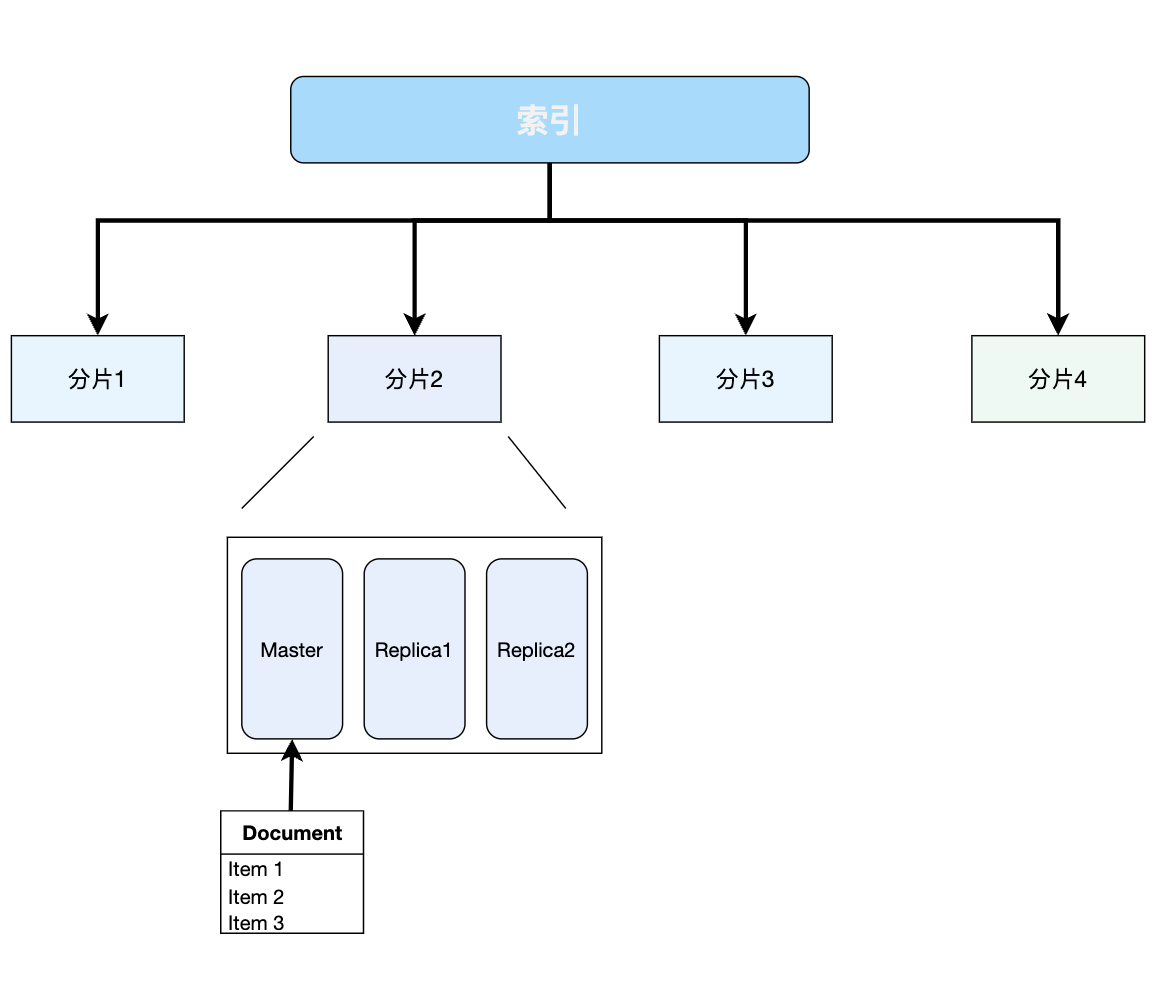
\includegraphics[width=0.6\linewidth]  {Elasticsearch.png}} 
	\caption{Elasticsearch结构}
	\label{es}
\end{figure}
如图\ref{es}所示,Elasticsearch 集群是由多个节点构成的,每个节点可承载一个或者多个分片,集群里的数据是以索引作为单位来组织的,每个索引都包含一组有相似结构的文档,并且采用统一的映射实施管理,在多语言代码检索系统当中,可以针对不同的编程语言或者项目类型分别创建索引,也可把所有代码文件统一存放在一个索引里,这样方便进行统一检索以及管理。Elasticsearch 中的索引属于逻辑上的数据集合,而分片则是物理上的数据分布单元,\par
为实现分布式存储\cite{ref13.5}并提升系统的可用性与性能,Elasticsearch 引入了分片和副本的机制,每个索引可被划分成多个主分片,每个主分片又可以拥有一个或多个副本分片。主分片负责数据的写入以及主控,副本分片用于容错和负载均衡\cite{ref13.7},当某个节点出现故障时,副本分片可迅速接管,保证系统的高可用性以及数据安全,在代码检索系统里,针对数百万个开源项目文件,可以依靠合理配置分片和副本数量,优化系统的检索性能以及容错能力。\par
文档是 Elasticsearch 中可被索引和检索的最小数据单元,采用 JSON 格式进行存储,类似于关系型数据库中的一行数据,在代码检索场景下,一个文档一般对应一个具体的代码文件,包含文件名、代码内容、开源协议、星数等丰富的元数据信息,凭借灵活的映射配置,可以对不同类型的字段进行高效索引和检索。\par
Elasticsearch 提供了功能强大的 RESTful API\cite{ref13.9},便于与各类应用系统集成,还支持分布式部署、负载均衡、故障转移等企业级特性,保障系统的稳定性和可扩展性,Elasticsearch 内置了高效的全文检索、分词、聚合分析、排序和高亮显示等功能,支持多种复杂查询方式,包括关键词检索、布尔查询、短语匹配等。在代码检索系统中,可以结合代码结构化表达提取的特征进行索引,提升检索的准确性和相关性,依靠这些机制,Elasticsearch 可高效地管理和组织大规模的代码数据,全面支持分布式、高并发的代码检索需求。\par


\subsection{Transformer驱动的大规模预训练语言模型}
\zihao{-4} 
大语言模型是实现本系统搜索功能的核心技术。近年来,随着代码数据规模的爆炸式增长,传统的基于关键词和规则的代码检索方法已难以满足开发者对语义理解和智能检索的需求。大语言模型凭借强大的语义建模和理解能力,能够对代码片段、函数、类等多粒度代码实体进行深层次的语义表示和推理,从而极大提升代码检索系统的智能化水平。当前,基于大语言模型的代码检索系统已成为智能开发辅助、代码推荐、自动补全等场景的关键基础设施。要深入理解当前的大语言模型,必须先了解其核心架构——Transformer。因此,本节将简要介绍Transformer及大语言模型的其他关键技术,并结合其在代码检索系统中的应用进行说明。

\subsubsection{Transformer}
Vaswani\cite{ref14}等人指出,循环神经网络模型\cite{ref14.5}在每个时间步都需要依赖前一时间步的隐藏状态信息进行计算,这种固有的顺序依赖性使得RNN难以在多GPU上进行并行计算,从而限制了RNN在处理超大规模文本数据时的训练能力。为了解决这一问题,他们提出了Transformer架构,这是一种完全依赖注意力机制连接编码器和解码器的网络架构。Transformer显著提高了训练的并行度和速度。后续的一系列研究表明,基于Transformer架构的预训练模型在各种任务上都能实现最先进的性能表现,因此,Transformer已成为自然语言处理领域的首选架构。除了在语言相关领域的应用之外,Transformer还被广泛应用于计算机视觉、音频处理以及自然科学学科,如化学、生物等领域。\par
Transformer\cite{ref14.7}架构如图\ref{transformer}所示,其整体由编码器(图\ref{transformer}左)和解码器(图\ref{transformer}右)组成。每个编码器块由多头注意力机制模块和位置前馈网络组成,模块间使用残差连接,并配有层归一化模块;解码器块在位置前馈网络和多头自注意力模块之间插入了交叉注意力模块,其中的自注意力模块用于组织某个位置信息对后续位置信息的影响。下面将简要介绍上述几种重要模块:\par
(1)多头注意力机制:让序列中的每一个元素学习并计算与其他元素的互注意力分数权重,如公式\ref{func_1}所示:
\begin{eqnarray}
	\text{Attention(Q,K,V)} =  \text{softmax}(\frac{QK^T}{\sqrt[]{d_k}})V
	\label{func_1}
\end{eqnarray}
但Transformer并不只是简单应用了单个注意力函数,而是使用了多头注意力机制将 \(d_m\) 维度的原始 \(Q\)、\(K\)、\(V\) 分别线性投影到 \(d_k\)、\(d_k\)、\(d_v\) 维度,再根据公式\ref{func_1}进行注意力计算,整体公式如下:
\begin{eqnarray}
	\mathrm{MultiHead(Q,K,V)=~Concat(head_{1},...,head_{h})W^{O}} \\
	\mathrm{where~head_{i}~=~Attention(QW_{i}^{Q},KW_{i}^{K},VW_{i}^{V})}
	\label{func_2}
\end{eqnarray}
Transformer利用多头注意力机制能够同时关注到来自不同位置的且具有不同表示的子空间信息,增强了架构的表达能力。\par
(2)位置前馈网络:全连接前馈网络模块,用于接收自注意力模块的输出:\par
\begin{eqnarray}
	\mathrm{FFN}(x) & =\max(0,x\mathrm{W}_1+\mathrm{b}_1)\mathrm{W}_2+\mathrm{b}_2 \\
	& =\mathrm{~ReLU(H'W}_1+\mathrm{b}_1)\mathrm{W}_2+\mathrm{b}_2
	\label{func_3}
\end{eqnarray}
(3)残差连接与归一化:Transformer 在每个模块间使用残差连接,然后进行层归一化。其中编码器块表示为:\par
\begin{eqnarray}
	\mathrm{H^{\prime}=~LayerNorm(Self~Attention(X)+(X)} \\
	\mathrm{H=~LayerNorm(FFN(H^{\prime})+(H^{\prime})}
	\label{func_4}
\end{eqnarray}
\begin{figure}[H] 
	\center{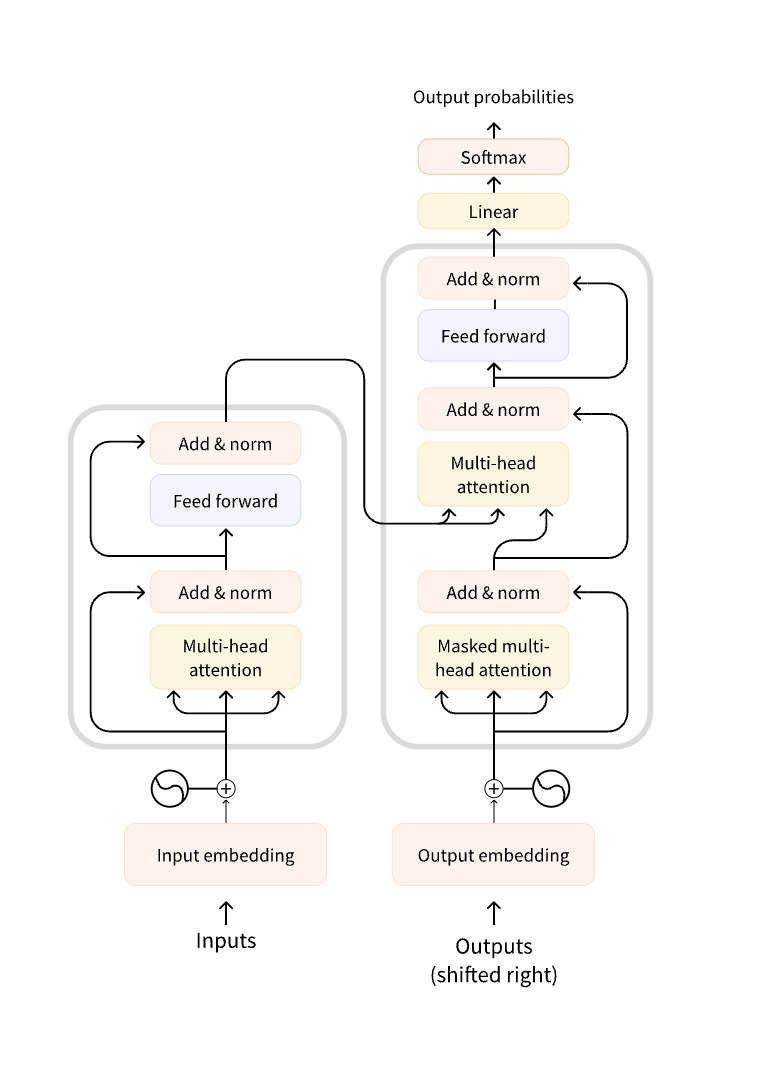
\includegraphics[width=0.4\linewidth]  {transformer.png}} 
	\caption{Transformer结构}
	\label{transformer}
\end{figure} %图表上下各空一行
基于Transformer的大规模预训练语言模型能够对自然语言查询和代码片段进行统一的语义建模,实现跨语言、跨风格的代码理解与检索。在代码检索系统中,大语言模型通常作为语义编码器,将用户的自然语言查询和代码库中的代码片段映射到同一语义空间,通过向量相似度检索相关代码。这种方法突破了传统基于关键词的检索方式,能够理解复杂的语义关系和上下文信息,显著提升了代码检索的准确率和智能化水平。此外,大语言模型还可用于代码摘要生成、代码补全、错误修复等多种智能开发场景,极大丰富了代码检索系统的功能边界。

\subsubsection{面向任务自适应的混合专家深度学习框架}
\begin{figure}[H]
	\center{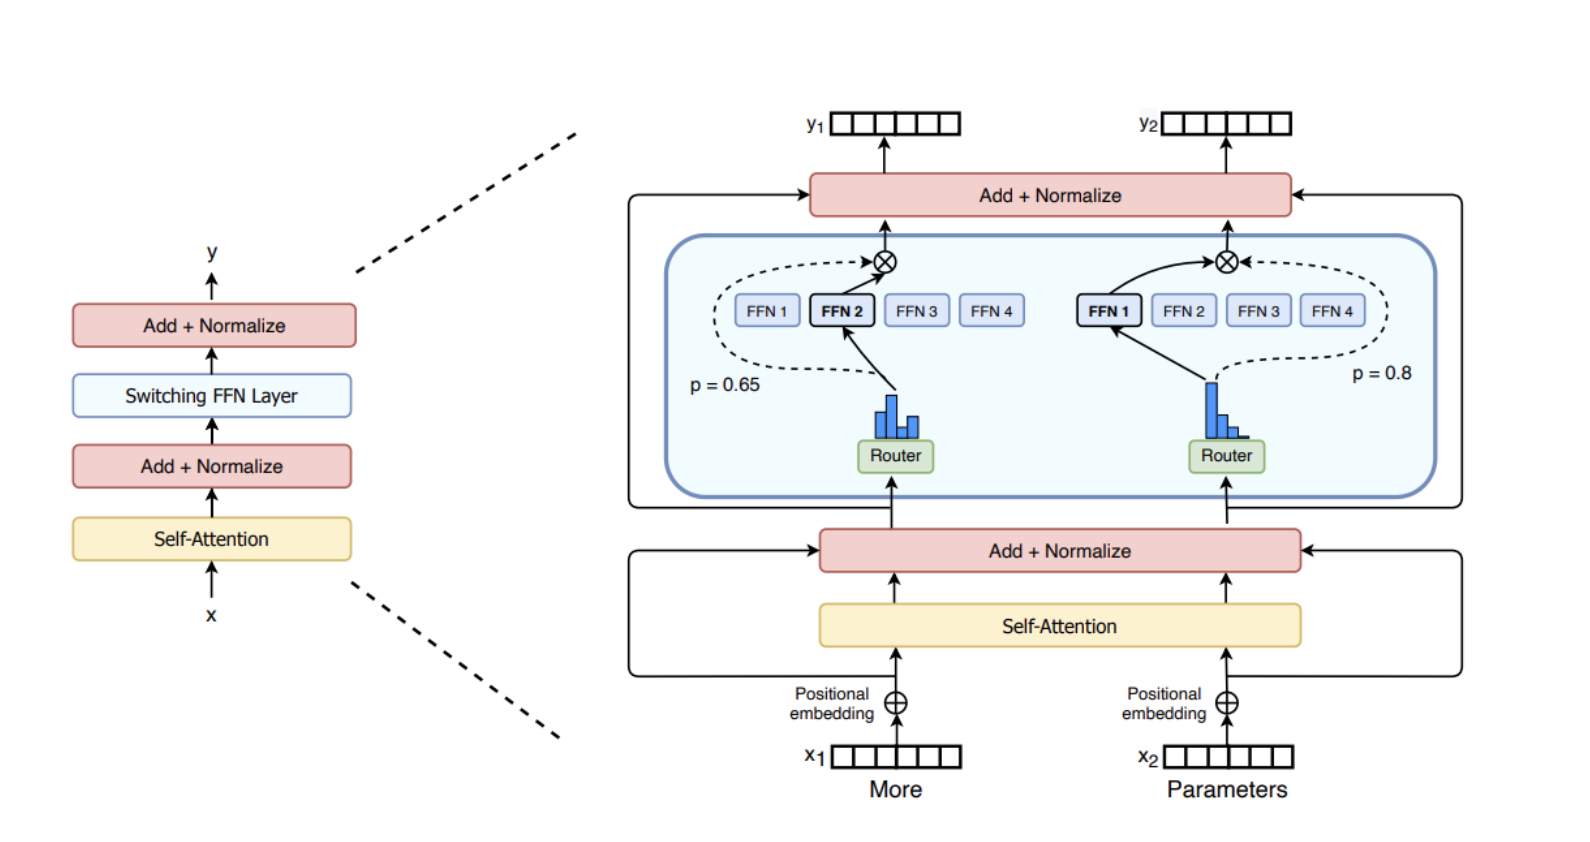
\includegraphics[width=0.95\textwidth]  {MoE.png}} 
	\caption{MoE结构}
	\label{MoE}
\end{figure}
Google Brain团队察觉到传统Transformer架构在扩展至超大规模时会碰到计算资源消耗急剧增加的状况,前馈网络层的全参数激活机制致使训练和推理效率大幅降低,鉴于此,他们提出了基于混合专家模型\cite{ref15}的稀疏架构改造举措,依靠把Transformer里的FFN层替换成动态路由的专家网络集合,达成计算效率与模型容量的平衡。MoE架构如图\ref{MoE}所示,其核心创新之处在于引入稀疏门控机制,该机制由可学习的路由网络组成,针对每个输入词元生成专家选择概率分布,仅仅激活概率最高的前K个专家,其余专家维持非激活状态,展开来说,每个MoE层包含N个独立的前馈网络作为专家,其数学表达为:
\begin{eqnarray}
	\mathrm{MoE}(x)=\sum_{i=1}^KG(x)_i\cdot E_i(x)
	\label{func_5}
\end{eqnarray}
其中$G(x)$是门控网络输出的Top-K权重,$E_i(x)$是被选中的专家网络输出。这种设计让模型总参数量可扩展到万亿级别,而实际计算量只和激活专家数有关,实验显示,Switch Transformer在同等计算资源情况下,训练速度比传统稠密模型提高了4倍,并且推理时内存占用降低到1/4,凭借引入噪声注入和负载均衡损失函数,MoE有效缓解了专家利用率不均衡问题,例如GLaM模型以1.2万亿参数仅激活97亿参数就达到了GPT-3的97\%性能。当下MoE架构已在GPT-4、DeepSeek、Mixtral 8x7B等主流大模型中广泛运用,成为突破单一模型规模瓶颈的核心技术路径。

\subsubsection{基于语义增强的大模型提示工程}
提示也就是一系列给予大语言模型的指令,可借由自定义提示来提高以及改善大语言模型的能力,Schulhoff等人在参考文献\cite{ref16}中系统性地提出Prompt是调控大型语言模型行为的核心接口,其本质是借助自然语言指令或者结构化模板明确输入规范、处理规则以及输出约束,动态重构大语言模型的上下文推理路径来适配特定任务需求。举例来说,可以让大语言模型在生成文档时标记重点内容,可让大语言模型只输出符合要求的关键词语,还可以让大语言模型只生成指定代码风格的代码等等。提示工程作为一种独特的编程模式,主要是围绕向大型语言模型精准输入提示来开展操作,从本质上讲,这需要精心设计适配的提示模板,以此来帮助完成特定的下游任务。实践证明,优化提示内容可提升模型在各类任务中的表现。\par

\begin{figure}[H]
	\center{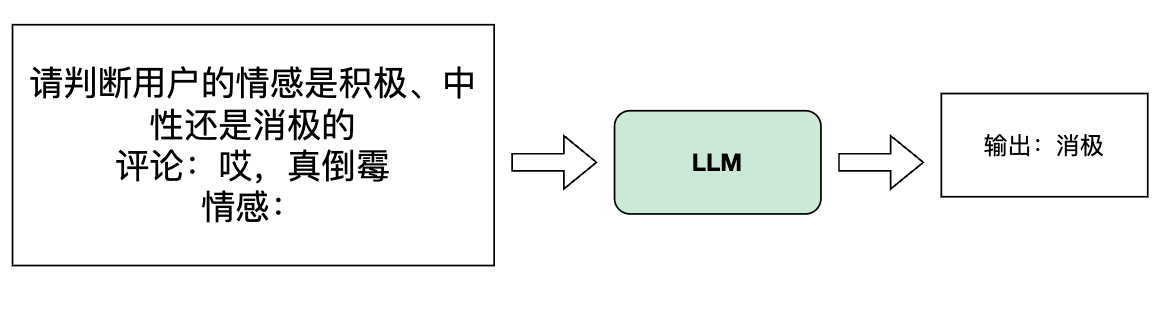
\includegraphics[width=0.95\textwidth]  {zero_shot.png}}
	\caption{零样本提示示例}
	\label{zero_shot}
\end{figure}
\begin{figure}[H]
	\center{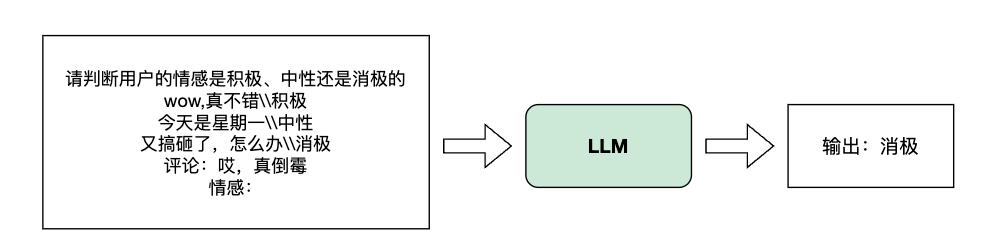
\includegraphics[width=0.95\textwidth]  {few_shot.png}}
	\caption{少样本提示示例}
	\label{few_shot}
\end{figure}

在提示工程实际运用里,零样本提示\cite{ref17}属于一种基础方法,图\ref{zero_shot}呈现了相关示例,在此方法下,就算不向模型提供任何参考示例,模型也可给出有价值的回应,完成定任务,不过当零样本提示无法契合需求时,少样本提示\cite{ref18}就发挥作用了,如图\ref{few_shot}。这时要针对下游任务设计专门的提示模板,模板要包含一系列大语言模型处理规则,还要为后续待输入文本预留特定位置,向大语言模型发起询问时,只要把待输入文本填充到提示模板预留空位,就能构建完整提示,另外开启思维链、给大语言模型指定角色性格等提示技巧可改变大语言模型输出效果和对任务的执行情况。\par
而言,巧妙构建提示可产生全新的交互模式,借助提示指令,大语言模型可生成与软件工程概念相关的测验题目,模拟程序运行流程,甚至模拟命令行终端窗口的交互场景,而且提示有自适应特性,部分提示可依据当前情况,推荐其他提示,以便收集更多信息,或生成相关成果物,提示的这些进阶功能,充分说明了深入设计提示、挖掘其在简单文本与代码生成之外价值的关键性。\par
在代码检索系统中,提示工程可用于优化自然语言查询的表达方式,还可以引导大语言模型理解用户意图,实现更精准的代码匹配,凭借设计针对代码风格、功能描述、编程语言等维度的提示,能让大语言模型在检索和生成代码时更贴合实际开发需求,提示工程还可用于多轮对话、代码解释、错误定位等场景,提升代码检索系统的人机交互体验和智能化水平。\par

\subsection{基于微服务的高可用后台架构}
\zihao{-4}
微服务架构属于本系统达成的关键技术之一,与之相对的是传统的单体架构方案,单体架构\cite{ref18.5}如图\ref{compare}左所示,把整个系统封闭于一个程序内,整合了登录、鉴权、业务逻辑、数据处理等全部功能模块,这种“大而全”的架构对于小型系统来讲,可缩短开发周期,并且开发和部署流程比较简单,契合开发者的直觉与习惯。不过随着系统规模的增大以及业务复杂度的提高,单体架构渐渐显露出模块耦合度高、扩展性差、维护成本高等问题,很难契合高并发、大数据量以及多语言支持等现代应用场景的需求,\par
相较而言,微服务架构运用了“高内聚、低耦合”的设计观念,如图\ref{compare}右所示,微服务将系统的各个功能模块拆分成独立的服务,每个服务专心于完成某一特定功能,并以单独的进程或者容器形式运行。整个系统由一组相互协作的微服务组成,服务之间借助网络进行通信,微服务架构的核心特性在于服务的颗粒度更精细,职责更为单一,利于独立开发、测试、部署以及扩展,一般状况下,每个微服务会运行在Docker容器中,而Kubernetes则负责对这些服务进行高效的管理与编排。凭借这种办法,微服务架构提升了系统的灵活性与可扩展性,还为大型复杂系统的开发和维护给予了更强的支持。\par
\begin{figure}[H]
	\center{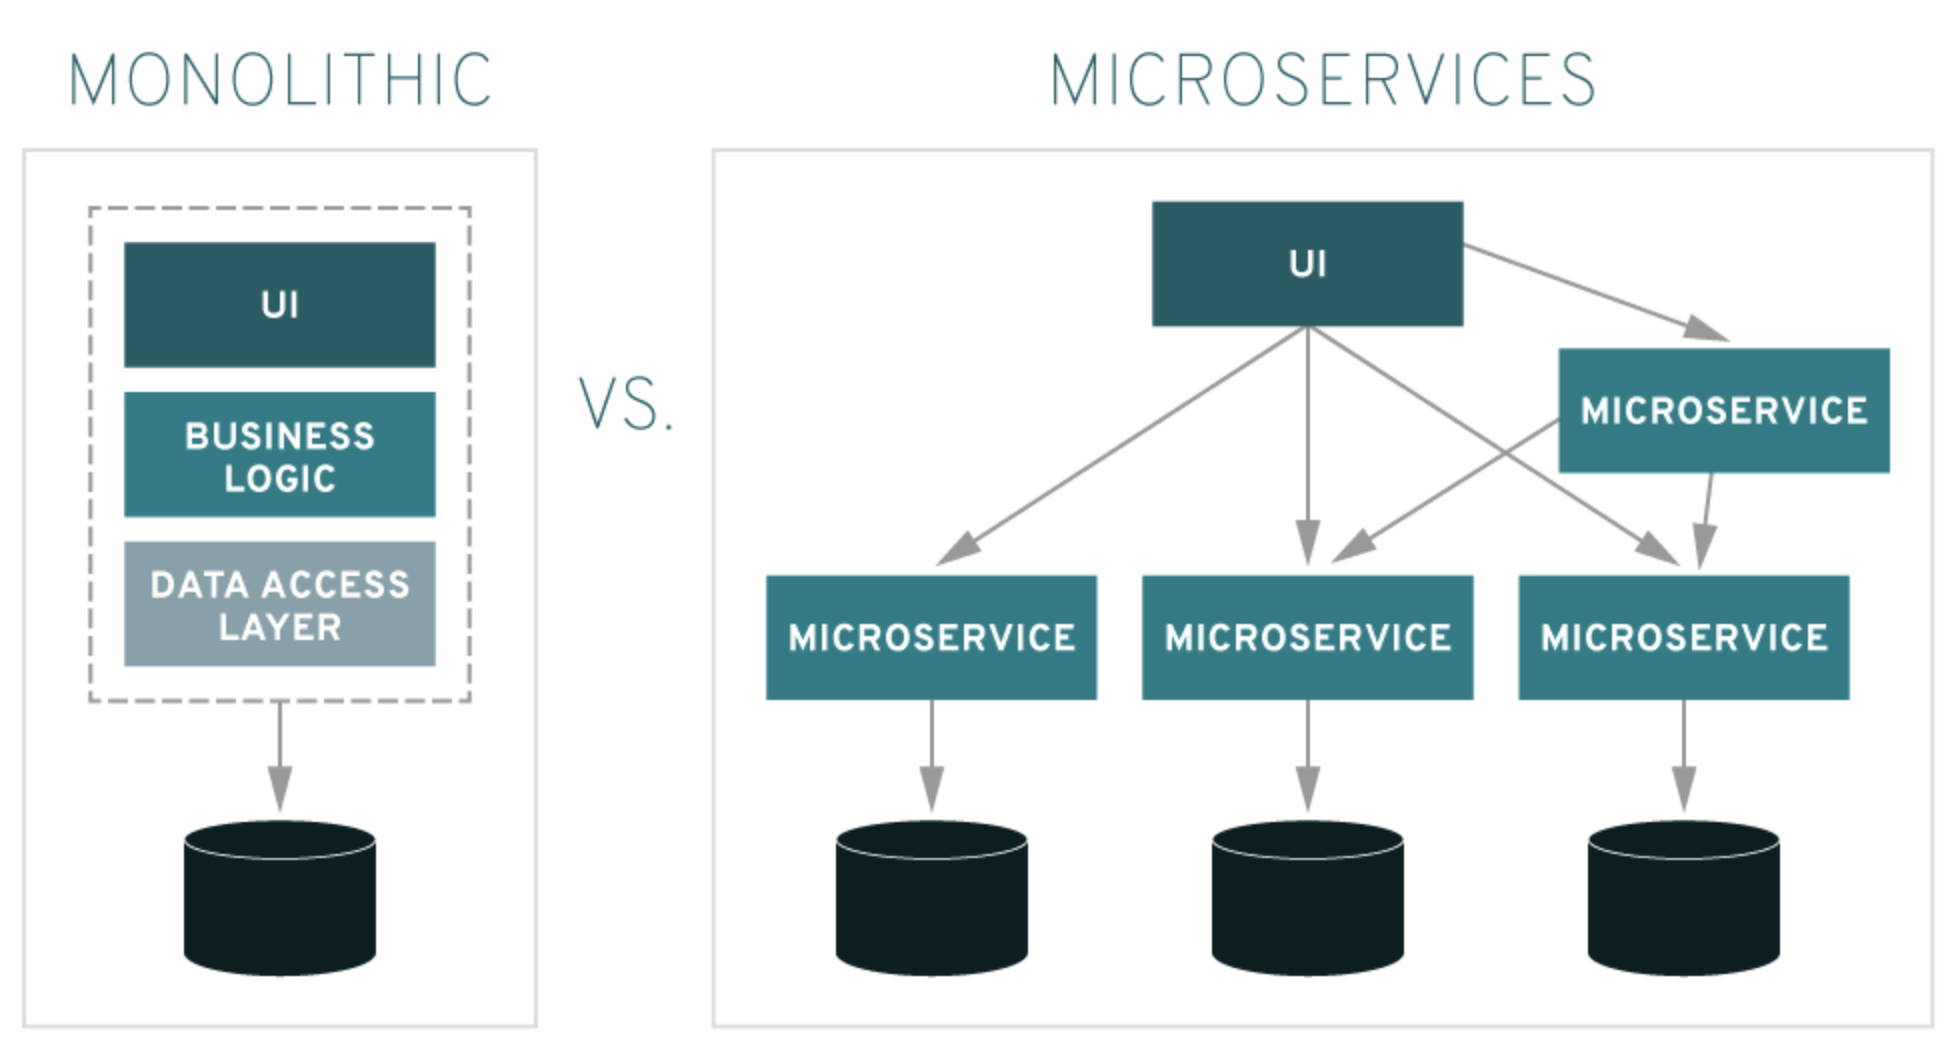
\includegraphics[width=0.5\textwidth]  {compare.png}} 
	\caption{单体架构和微服务架构对比}
	\label{compare}
\end{figure}
构建面向多编程语言的代码检索系统时,系统大多时候要处理多种编程语言的解析、索引、检索以及语义分析等复杂任务,并且还得依靠大模型来达成检索词的检索提高功能,不同编程语言的处理逻辑、依赖环境与扩展需求都不一样,单体架构很难灵活应对多语言场景下的异构需求,然而对于微服务来说,每个微服务可采用最契合其功能的编程语言和技术栈。比如说可用Python服务来部署大语言模型,以此实现系统里的检索提高功能,用Go语言搭建网关、鉴权、检索等服务可以应对高并发的请求处理以及业务的安全校验,如此一来提升了开发效率,又方便集成社区已有的多语言处理工具,同时针对不同模块的微服务,可独立扩展相关微服务的实例数,实现资源的动态分配以及弹性伸缩。像网关这类服务,往往是IO密集型而非CPU密集型,在部署时可考虑使用轻量级的容器实例进行横向扩展,以应对高并发的网络请求压力,而大语言模型推理服务,一般是计算密集型任务,可以部署在有GPU加速能力的节点上,并依据实际负载动态调整模型服务的副本数,实现资源的高效利用以及系统整体的弹性伸缩。另外微服务架构还支持服务的独立升级与灰度发布,当需要对某一编程语言的解析模块进行功能优化或者安全加固时,只需对对应的微服务进行迭代和部署,不用影响其他服务的正常运行,这种解耦的架构极大地降低了系统维护和演进的复杂度,提升了系统的可维护性与可用性,在多语言代码检索系统中,微服务架构还便于集成和管理多种第三方工具与智能组件。例如可以为不同编程语言分别集成专用的语法分析器、静态检查工具或者代码格式化服务,也可灵活接入多种大语言模型用于语义提高、代码补全或者自然语言查询理解,各服务之间凭借gRPC等高效协议进行通信,保证了系统的高性能与低延迟。\par
微服务架构为面向多编程语言的代码检索系统提供了高可用、高扩展性和高灵活性的基础设施保障,是支撑大规模、智能化代码检索服务的关键技术路径。\par

\subsubsection{跨语言的远程调用框架}
gRPC\cite{ref19}是一款有高性能特点且开源的跨语言远程过程调用也就是RPC框架,在微服务架构下的服务间通信方面有着广泛应用,gRPC能让客户端应用程序直接去调用服务器端应用的方法,仿佛那些方法就是本地对象一般,如此一来便让分布式应用程序开发变得更为简便,gRPC将HTTP/2用作传输协议,支持双向流以及头部压缩等特性,提供了更为高效的网络通信。gRPC借助Protocol Buffers来定义接口和服务,这是一种有轻量级特点且跨平台的消息格式,可提升数据交换效率同时减少带宽使用,在微服务架构里,gRPC因自身高效性而被广泛运用于服务间通信。\par
在gRPC当中,服务定义以及数据交换格式一般会使用Protocol Buffers。Protocol Buffers是由Google设计的一种有着轻量级特点且跨平台的消息格式,用于序列化结构化数据,借助.proto文件,开发者可定义自身的数据结构以及服务接口,这些定义会被编译成不同编程语言的代码,以便生成便于使用的类来构建强类型的请求和响应消息。和其他序列化协议比如JSON、XML、BSON等相比较,protobuf采用二进制编码,消息体积较小,传输高效,适合高并发以及大数据量场景,另外protobuf支持多种编程语言,gRPC自带的编译工具可快速生成多语言桩代码,适合多语言协作的微服务架构。而且protobuf凭借为字段分配唯一标识符,支持消息格式的平滑演进,保障了系统的长期可维护性。\par

\subsubsection{容器化部署与环境隔离基础设施}

Docker\cite{ref20}是一款开源的应用容器引擎,借助它开发者可把应用程序及其依赖一同打包进一个有可移植性的容器里,随后发布到任何一款流行的Linux或Windows机器上,并且还可达成虚拟化,容器运用沙箱机制,相互之间处于隔离状态,有较高的安全性,Docker容器所拥有的轻量化特性以及快速部署能力,使其成为微服务架构里的理想之选。每一个微服务都可被打包成一个独立的Docker容器,这样就保证了环境的一致性,同时也简化了开发、测试以及部署流程,另外因为Docker容器的资源消耗较少,多个容器可在同一台物理机上高效地共同存在,提高了资源利用率,Docker采用联合文件系统技术,如图\ref{docker}所示,将不同的文件系统层相互叠加起来,形成统一的视图。每个Docker镜像由一系列只读层构成,在创建容器时会在最顶层添加一个可写层,这种层次化设计加快了镜像构建以及分发过程,还提升了数据隔离性与安全性。\par
\begin{figure}[H]
	\center{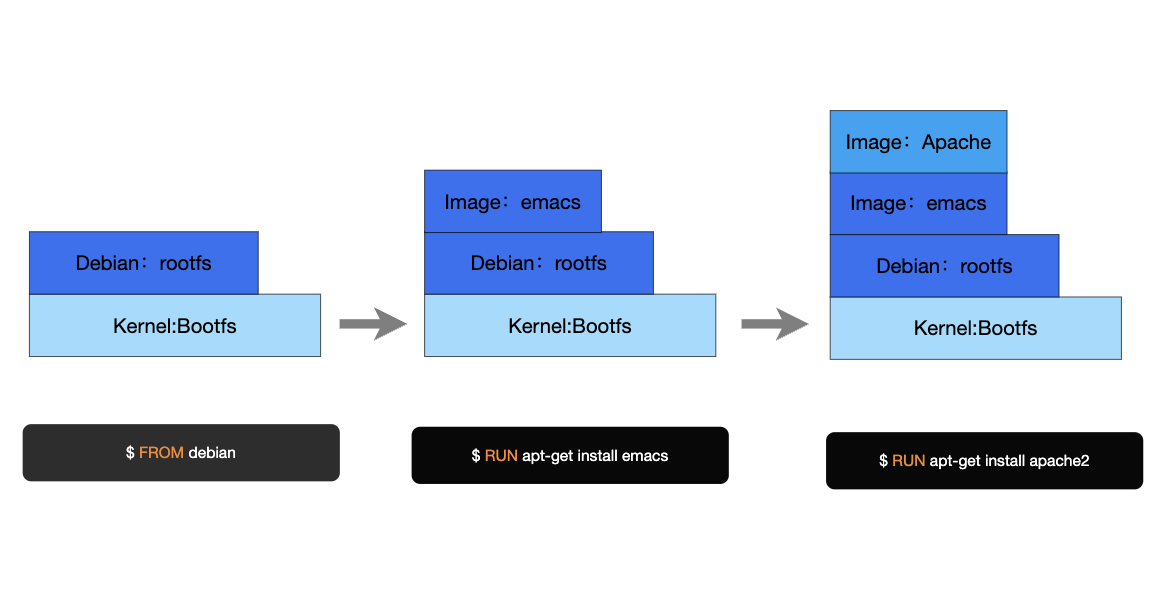
\includegraphics[width=0.8\textwidth]  {docker.png}} 
	\caption{docker层次化构建示例}
	\label{docker}
\end{figure}
\subsection{本章小结}
\zihao{-4} 
在这一章节当中,对面向多编程语言的代码检索系统所涉及的核心理论以及技术给予了介绍,最先阐述的是代码检索问题的基本内涵,以及其于现代软件工程里有的意义,跟着针对分布式高性能搜索引擎在大规模代码数据管理以及高并发检索方面的应用优势展开了详细说明,这为系统的可扩展性与高可用性给予了有力支持。于智能检索层面,着重剖析了以Transformer作为代表的大规模预训练语言模型的原理,以及其在代码语义建模、跨语言检索等场景中的应用价值,还介绍了混合专家模型等前沿深度学习架构在提升模型容量以及推理效率方面的创新之处,以及基于提示工程的语义提高方法对大语言模型能力的优化与扩展。借助这些技术,系统可达成对自然语言查询以及多语言代码的统一语义理解,使得检索的准确性与智能化水平得以提升,在系统架构方面,讲述了微服务架构于多语言代码检索系统中的关键作用,微服务凭借服务解耦、异构技术栈支持、弹性伸缩以及高可用性,极大地提升了系统的灵活性与可维护性。结合gRPC、Docker等云原生技术,达成了高效的服务通信、环境一致性,契合了大规模、复杂业务场景下的高并发以及持续演进需求,总的来说,这一章节为后续系统设计与实现奠定了坚实的理论基础以及技术支撑,明确了多语言代码检索领域的研究趋势与技术挑战,为构建高效、智能、可扩展的代码检索平台提供了全面的指导与参考。
\newpage
\fancyhead[LH]{\zihao{-5}{\songti 重庆大学本科学生毕业论文(设计}}
\fancyhead[RH]{\zihao{-5}{\songti 3\quad 系统需求分析与设计实现}}
\section{面向多编程语言的代码检索系统需求与设计}
\subsection{面向多编程语言的代码检索系统需求分析}
\subsubsection{用户需求}
在本系统设计开发进程里,用户需求分析一直是需求工程的关键与根基,面向多编程语言的代码检索系统,其目标用户群体主要有软件开发者、编程学习者等多种人群,对不同用户实际使用场景加以梳理,能发觉他们对代码检索系统的需求有一定共性,也各有侧重点,以软件开发者而言,在日常开发进程中,在实现标准业务模块或者要完成某些特定功能时,大多时候会碰到需参考行业最佳实践或标准实现方式的情形。比如开发者接入某个数据库时,可能要查找该数据库在不同编程语言下的SDK接入示例,或者实现分布式系统时,想了解某种语言下CAS锁的标准写法,又或者实现轮询器、消息队列等通用组件时,期望能借鉴社区中成熟的代码片段,这些场景下,开发者一般希望能快速检索到高质量、可复用的代码实现,减少重复劳动的时间和精力。而对于编程学习者来说,代码检索系统的主要用途体现在学习和练习进程中,比如刷算法题、完成课程作业或自学新技术时,遇到难以独立实现的功能,便希望依靠检索系统查找相关代码片段进行参考学习,加深对知识点的理解与掌握。\par
具体到功能方面,用户普遍期望能依靠自然语言描述或者简洁关键词输入,快速定位到与自身需求高度契合的代码片段或完整项目实现。由于实际开发和学习进程中涉及的编程语言种类众多,用户往往要跨语言、跨项目查找解决方案,系统要有多编程语言检索能力,且能根据用户输入自动识别目标语言、相关API、开源协议等关键信息,检索结果的展示方式也颇为关键,用户希望系统能以直观、结构化界面呈现检索结果,便于快速浏览和对比不同实现方案。对于感兴趣的代码片段,用户还希望能查看其所属项目的详细信息,涉及项目描述、开源协议、星标数量、文件结构等,以便综合评估代码的可用性、合规性和维护性,另外部分用户开发者群体,还希望能将检索到的代码片段直接集成到本地开发环境中,或者借助VS Code插件实现一键插入和复用,提高开发效率和体验。\par


\begin{figure}[H]
	\center{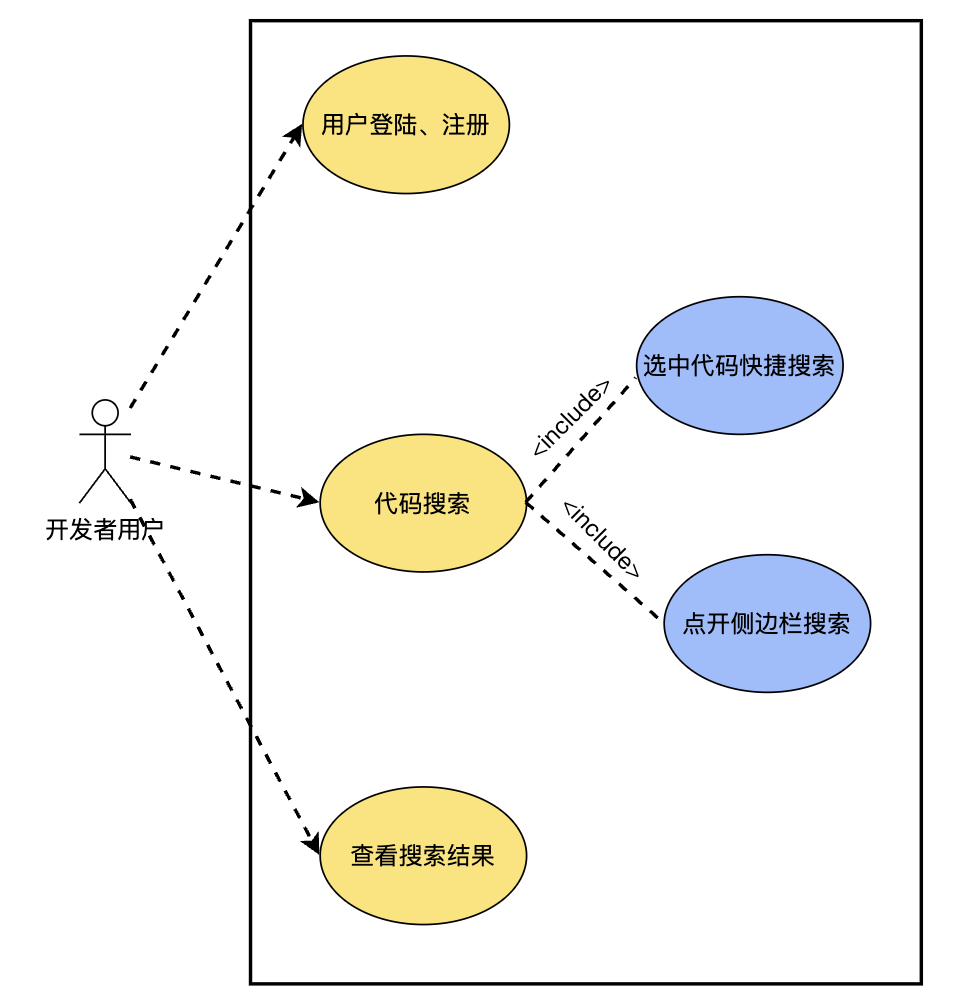
\includegraphics[width=0.5\textwidth]{user_use.png}}
	\caption{面向多编程语言的代码检索系统用户用例图}
	\label{usecase}
\end{figure}
在用户权限以及数据安全领域,用户一般较为关注个人信息和检索历史的安全与隐私状况,期望系统可给出完备的注册、登录以及身份认证机制,以此防止未获授权的访问以及数据的泄露,经过上述一系列分析,本文借助用例图,也就是图\ref{usecase}所展示的内容,针对主要用户需求开展了建模工作,涉及代码检索、项目详情查看、用户注册登录、权限管理等核心用例。每一个用例都对应着特定的用户操作流程以及系统响应情况,以此保障需求分析的完整性以及可追溯性,为后续系统设计与实现奠定了坚实基础。\par
\subsubsection{功能需求}
凭借对用户需求细致分析,面向多编程语言的代码检索系统要实现一系列核心功能,以此支撑用户在多语言、多场景下高效进行代码检索与复用,主要功能需求有以下几个方面:\par
系统得有强大的代码检索功能,用户可凭借自然语言描述、关键词输入或者代码片段示例,发起多编程语言的代码检索请求。系统要支持对主流编程语言像Python、Java、Go、C++、JavaScript等的代码片段、函数、类、模块等多粒度对象的检索,还可依据用户输入自动识别目标语言、相关API、开源协议等信息,检索功能需支持模糊查询、精确匹配、语义扩展等多种检索模式,以此提升检索的灵活性与准确性。\par
系统要支持项目详情查看功能,对于每个检索到的代码片段,用户可查看其所属项目的详细信息,覆盖项目名称、描述、开源协议、星标数量、文件结构、原始链接等,系统要支持对项目文件的层级浏览以及快速定位,方便用户深入分析项目实现和依赖关系,在用户管理与权限控制方面,系统要提供完善的用户注册、登录、身份认证和会话管理功能。支持用户信息的安全存储以及加密传输,防止未授权访问和数据泄露。\par
系统要支持VS Code插件集成,用户可以依靠VS Code侧边栏或者快捷键,直接在本地开发环境中发起代码检索、预览和插入操作,达成Web端与本地端的无缝协同,较大提升开发效率和用户体验。\par

\subsubsection{非功能需求}
除了上述提到的核心功能需求之外,面向多编程语言的代码检索系统还需要契合一系列非功能性需求,以此来保障系统拥有较高的可用性、可扩展性以及良好的用户体验,主要的非功能需求覆盖以下几个方面:\par
系统需要有良好的性能表现,在高并发访问的场景当中,系统要可在秒级的时间内对用户的检索请求做出响应,以此保证检索结果的实时性以及交互的流畅性。为了达成这个目标,系统后端需要采用高性能的分布式查询引擎,并且结合缓存、异步处理等优化手段,提升整体的吞吐量以及并发处理能力,对于大规模的代码数据集,系统要支持分布式存储与索引,以此保证数据可得到高效的管理以及快速的检索。\par
系统应有良好的可扩展性,随着用户规模以及数据量的持续增长,系统要可凭借横向扩展,比如增加服务器节点、微服务实例等方式来实现弹性扩容,避免出现单点瓶颈和性能瓶颈。系统架构应该采用微服务化设计,各个服务单元可独立进行部署、升级以及扩展,方便后续功能的迭代以及技术的演进。\par
系统需要有高可用性以及容错能力,为了保障系统在高并发、分布式部署以及节点故障等复杂场景下可稳定运行,系统应该引入服务注册与发现、负载均衡、健康检查、自动故障转移等机制,保证在部分节点出现故障时系统整体依然可正常提供服务。对于核心数据和服务,系统要支持多副本备份以及自动恢复,提升系统的鲁棒性以及可靠性。\par
系统要支持多端一致性以及跨平台兼容性,不管用户是凭借Web端还是VS Code插件来访问系统,都应该获得一致的功能体验以及界面风格,系统前端要适配主流浏览器和操作系统,后端要支持多种开发环境以及部署平台,以此提升系统的适用范围以及用户覆盖面。\par


\subsubsection{其他需求}
除了功能和非功能需求以外,面向多编程语言的代码检索系统还要关注安全性、可维护性、易用性等其他关键需求,以此提升系统的综合竞争力以及用户满意度,系统的安全性需求十分关键,系统要采用HTTPS协议加密所有前后端通信,避免数据在传输过程中被窃取或者篡改,用户密码等敏感信息要采用哈希加密存储,防止数据库泄露产生安全风险。系统要实现完善的身份认证与权限校验机制,防止未授权访问以及会话劫持等安全威胁,系统的可维护性需求体现在架构设计、代码规范和文档完善等方面,系统采用分层、模块化的架构设计,各功能模块职责清晰、接口标准,方便后续的功能扩展以及技术升级,系统代码要遵循统一的编码规范和注释标准,提高代码的可读性以及可维护性。另外系统的易用性需求直接影响用户的使用体验,系统界面应简洁直观,操作流程清晰,对于新用户,系统要提供友好的注册、登录和引导流程,降低上手门槛,另外系统还应遵循相关的开源协议和数据使用规范,尊重原作者的知识产权和数据隐私。\par
\subsection{面向多编程语言的代码检索系统设计方案}
\subsubsection{系统总体架构设计}
面向多编程语言的代码检索系统在整体组织上会采用前后端分离的模式,该系统主要囊括前端交互层、后端逻辑层以及数据层这三个层面,具体结构如图\ref{all_structure}所示,其中前端交互层借助Vue框架来编写交互逻辑,凭借ElementUI对前端图形化页面以及可视化模块给予渲染。后端则选用Gin框架并结合gRPC框架来编写应用服务,以此规范API风格,接收来自前端的请求,同时还要负责与数据层以及大语言模型展开交互,达成主要的搜索逻辑,数据层运用Elasticsearch对所有项目数据进行管理。\par
\begin{figure}[H]
	\center{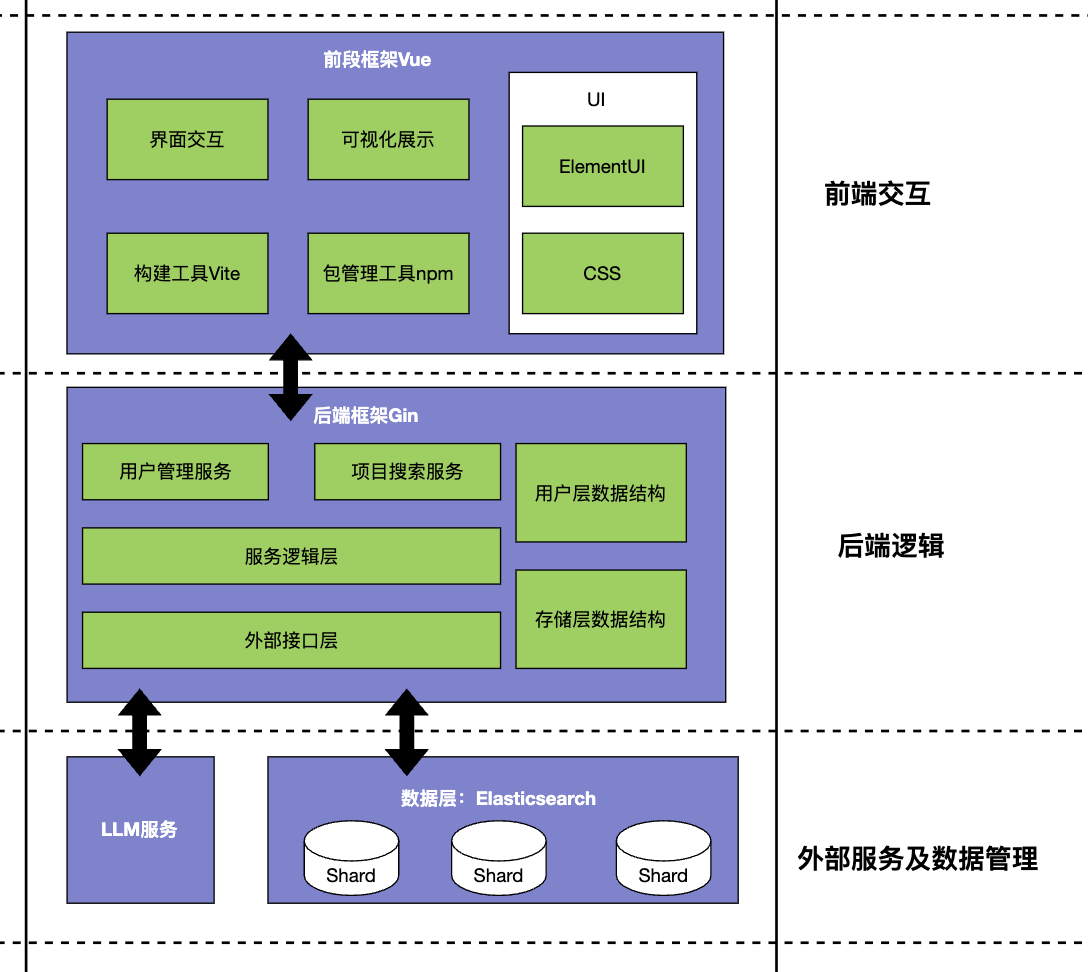
\includegraphics[width=0.4\textwidth]  {structure.png}} 
	\caption{系统总体架构图}
	\label{all_structure}
\end{figure}
\subsubsection{基于AST的代码结构化预处理设计}
代码结构化表达方式指的是把源代码从原本的文本形式转变成能体现其语法结构以及语义信息的形式化表示,和普通文本不一样,源代码有着严格的语法规则以及层次化的结构,仅仅依靠表层的字符串匹配很难捕捉到代码的深层含义,怎样对代码进行结构化建模,是达成高效且准确的代码检索与理解的基础。在软件工程的实践过程中,我们大多时候会运用AST这样的静态分析手段来对代码进行结构化的表达。\par
AST是代码结构化表示里较为常用的方法之一,AST用树状结构描述源代码的语法结构,把代码分解成语法单元,并且以节点的形式组织起来,借助AST,可以有效地捕捉代码的层次关系以及语法特征,方便后续的代码分析、转换以及检索。一般抽象语法树以代码中的条件判断分支当作树的节点,说AST是抽象的是因为树上的每个节点不代表任何一种具体语言的具体条件控制语句,仅仅代表节点本身所映射的条件控制逻辑,比如“如果”“循环”等。\par
\begin{figure}[H]
	\center{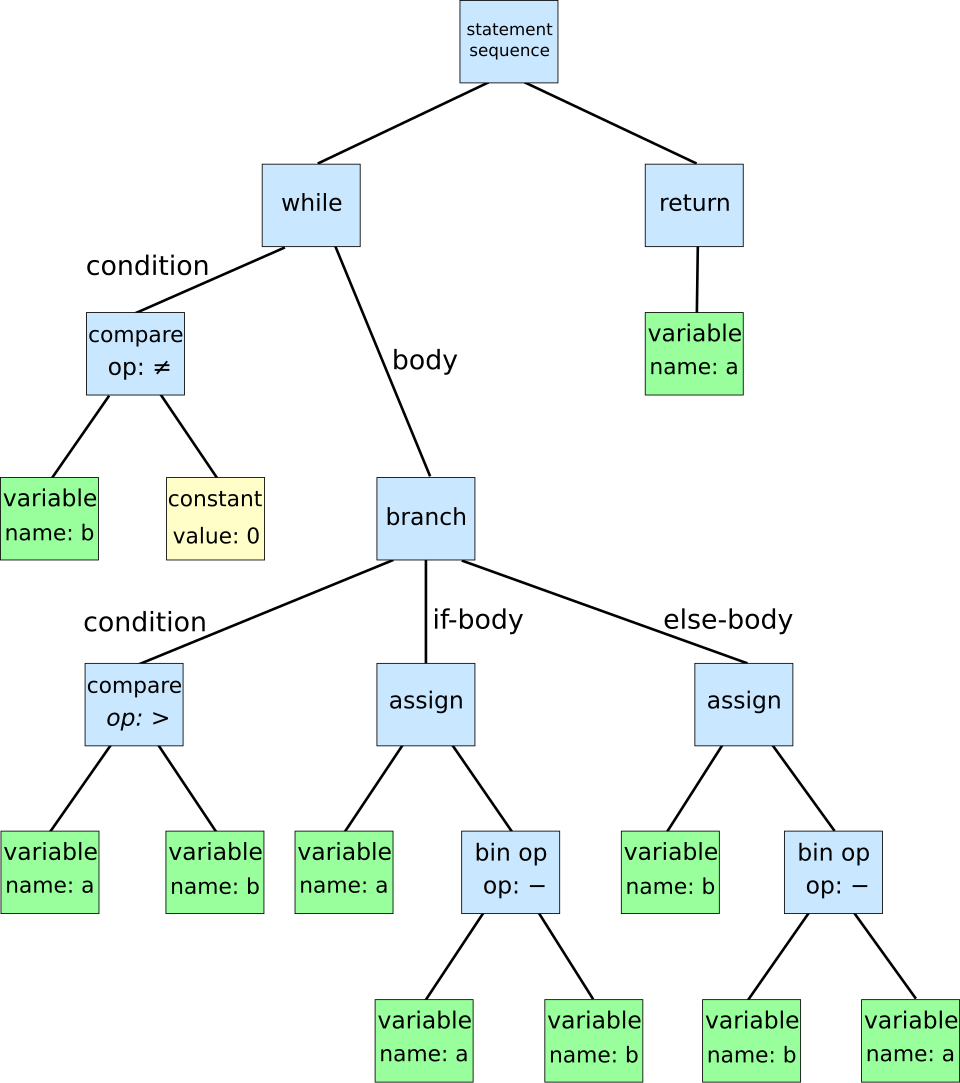
\includegraphics[width=0.4\textwidth]  {ast.svg.png}} 
	\caption{抽象语法树示例}
	\label{ast}
\end{figure}
一个常见的语法树如图\ref{ast}所示,图中的“while”“compare”都表示实际代码中的具体控制逻辑,不过该抽象语法树并未映射任何语言。依靠抽象语法树,可高效地分析出代码的具体控制结构,因为AST本质上是一种抽象的语法表示,不依赖于具体编程语言的语法细节,借助对不同语言的AST进行归一化处理,可以实现跨语言的结构对齐以及统一建模,为多语言代码检索以及迁移提供基础,由于大部分的代码结构都比较规范,使用AST可很好地适配较多数的代码。并且因为AST采用树状图的结构对代码进行分析,可便于对代码的层次关系以及控制结构进行分析,基于AST可以实现对完整项目的具体拆解,使得代码搜索的颗粒度得到细化,可可代码检索系统实现跨语言搜索的特性,为此本文打算采用主流的开源AST解析工具,对不同编程语言的项目源代码进行统一的结构化预处理。依靠AST分析,可以有效揭示代码的层次结构与语义关系,为后续的特征提取和检索任务提供坚实的数据基础。
在本项目里,代码预处理计划分成三个阶段,首先是代码收集阶段,系统借助自动化工具从开源代码托管平台批量抓取多种编程语言的代码仓库,为保证数据有多样性与代表性,收集范围包含主流编程语言像Java、Python、Go、JavaScript等,并且优先挑选活跃度高、星标数量多的项目,以此保证代码质量和实用价值。自动化脚本会定期执行,能持续更新与扩充代码库,契合系统对大规模、多语言代码数据的需求,收集过程中,系统还会抓取仓库的元信息,覆盖项目描述、开源协议、贡献者信息等,为后续的检索和筛选提供辅助数据支持,接着是结构化处理阶段,系统针对不同编程语言调用相应的开源AST解析工具,对收集到的源代码做语法分析,自动生成抽象语法树。这个过程实现了代码的统一结构化表达,方便进行跨语言的语义对齐和特征抽取,系统对生成的AST进行遍历和筛选,去除无关的冗余信息,比如注释、单元测试代码以及无实际业务逻辑的辅助函数,只保留核心功能实现相关的代码片段,为提升数据的一致性和可比性,系统会对AST节点进行规范化处理,包括统一节点类型命名、变量和函数标识符等。经过这一阶段处理,原始代码被转化为结构清晰、语义明确的中间表示,为后续的语义理解和检索提供坚实基础,最后是分析与存储阶段,系统会对结构化处理后的代码数据进行质量评估和统计分析,判断代码收集和预处理是否符合预期要求,凭借自动化脚本对代码的覆盖率、功能模块分布、语言比例等关键指标进行监控,及时发现可能存在的数据偏差或异常情况,保证数据集的完整性和代表性。符合质量标准的结构化代码及其对应的项目元信息会被统一存储于Elasticsearch数据库中,支持高效的索引和检索,该数据库保存代码的文本内容,还含有丰富的结构化信息,如函数签名、调用关系和代码注释等,可提升检索的准确性和响应效率。\par
\begin{figure}[H]
	\center{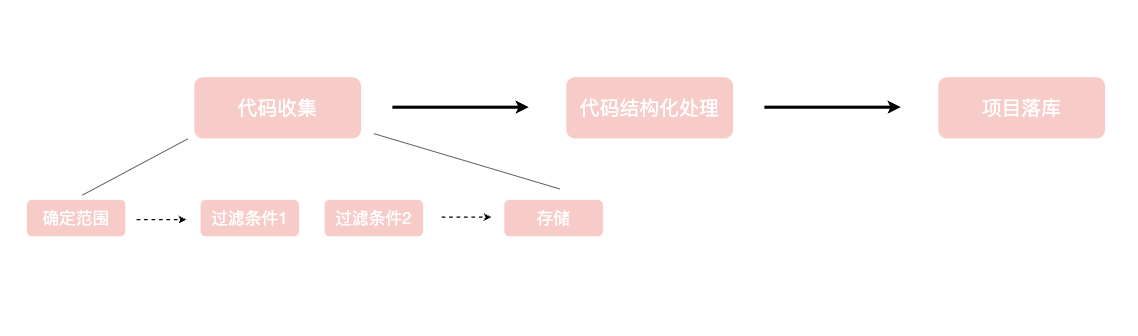
\includegraphics[width=0.95\textwidth]{pre_pro.png}}
	\caption{基于AST的代码结构化预处理设计}
	\label{pre_pro}
\end{figure}
总的来说,代码的结构化预处理过程就像图\ref{pre_pro}所展示的,使用AST进行代码结构化预处理流程是为了实现从代码采集、结构化转换到数据存储的全流程管理,为后续多编程语言代码检索系统提供高质量、结构化的数据支持。\par
\subsubsection{基于微服务的高可用后台分布式设计}

随着软件系统规模持续扩大以及业务复杂度不断提升,传统的单体式后端架构已经很难契合现代多编程语言代码检索系统对于高可用性、可扩展性以及灵活性的需求,微服务架构作为当下主流的分布式系统设计范式,把复杂系统拆解成一组松耦合、自治的服务单元,达成了服务的独立部署、弹性扩容以及高效协作,成为支撑大规模智能代码检索平台的关键技术基础。所谓微服务架构,就是将系统依据业务功能划分成多个独立的服务,每个服务围绕特定业务能力构建,有独立的数据存储和运行环境,并且借助轻量级通信机制来进行协作,和传统单体架构相比,微服务架构提升了系统的可维护性和可演化性,还极大提高了系统在高并发、分布式部署以及多语言支持等场景下的适应能力。在面向多编程语言的代码检索系统里,微服务架构可有效支撑多语言解析、智能检索、权限管理等异构服务协同运行,为系统的高可用性和弹性扩展提供坚实保障。\par
本节围绕高可用后台分布式技术的微服务架构展开,提出了一套系统化的后端设计方案,该方案以服务自治、弹性伸缩和容错机制为核心,结合分布式服务注册与发现、负载均衡、服务治理等关键技术,实现了多编程语言代码检索系统高可用、可扩展且易维护的后端支撑平台。整体方案覆盖以下两个阶段:\par
第一阶段是服务拆分与分布式部署,系统按照业务功能把后端划分成网关服务、鉴权服务、搜索服务、大语言模型服务等多个微服务单元,每个服务都可以独立开发、测试、部署以及扩容,极大提升了系统的灵活性和可维护性,依靠容器化技术和分布式编排平台,各服务可在多节点环境下弹性部署,实现资源的动态调度和高可用保障。服务间借助gRPC等高效通信协议进行数据交互,保证低延迟和高吞吐量。\par
第二阶段是高可用性与服务治理机制设计,系统引入分布式服务注册与发现机制,所有微服务在启动时自动向服务注册中心注册自身信息,其他服务可依靠注册中心动态发现并调用目标服务,提升系统的灵活性和容错能力。为应对高并发和突发流量,系统在网关层集成负载均衡策略,自动分发请求至后端多实例服务,避免单点瓶颈,各服务内部实现健康检查与自动故障转移机制,保证部分节点故障时系统整体仍能稳定运行,系统还支持灰度发布、自动扩缩容、日志追踪与链路监控等服务治理能力,为后续功能迭代和运维管理提供有力支撑。\par

\begin{figure}[H]
	\center{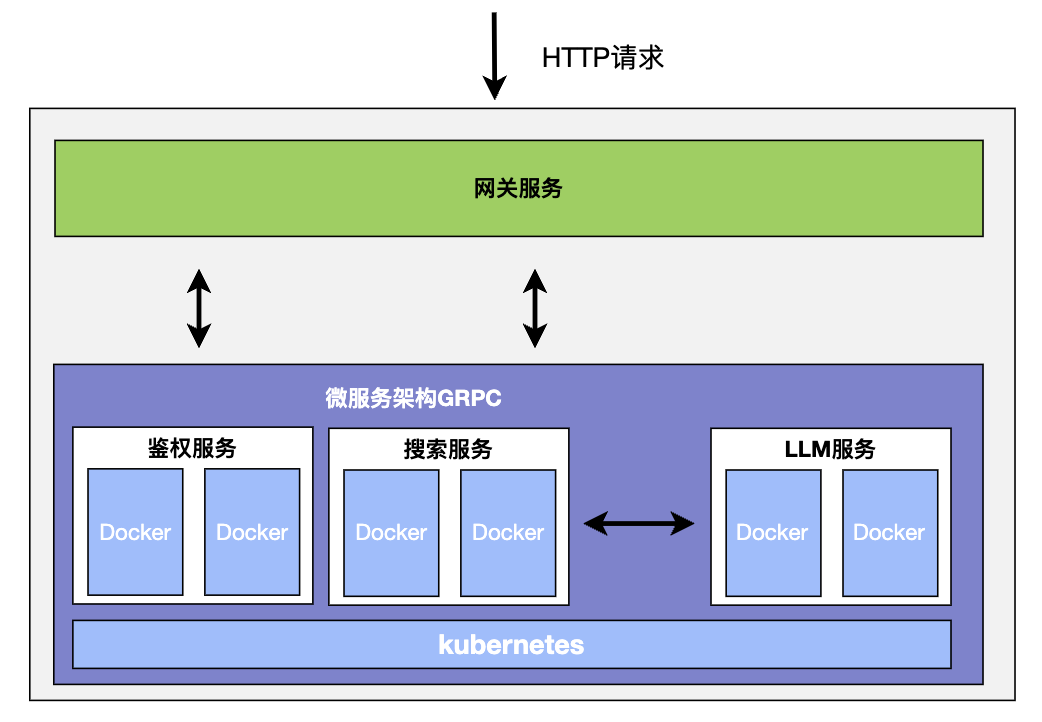
\includegraphics[width=0.95\textwidth]{back_model.png}}
	\caption{微服务架构下的高可用分布式后台结构}
	\label{microservice_arch}
\end{figure}
如图\ref{microservice_arch}所示的内容,是面向多编程语言的代码检索系统的整体后台架构,其中网关会统一对外给出API入口,承担请求路由、鉴权以及负载均衡等工作,鉴权服务专门负责用户注册、登录以及Token校验,以此保障系统安全,搜索服务和大语言模型服务相互协作,达成多语言代码的查询上下文提高以及智能检索。所有服务都支持多实例部署,借助容器编排平台达成弹性扩容以及自动恢复,提升系统的高可用性和并发处理能力。\par
\subsubsection{基于提示词工程的查询上下文增强技术}
随着大语言模型在自然语言处理以及代码智能领域被广泛运用,提示词工程渐渐变成提升模型性能与用户体验的一项关键技术,所谓提示词工程,指的是针对特定任务或者应用场景,系统地设计、优化以及管理输入给大语言模型的提示,以此引导模型生成更符合预期的输出结果,和传统的模型训练以及微调方法不一样,提示词工程不需要对模型参数进行修改,而是借助调整输入内容和结构,充分挖掘并利用预训练模型的知识与推理能力。在基于大语言模型的多编程语言代码检索系统里,提示词的设计与优化对检索效果有着决定性的影响,在处理跨语言、跨领域的复杂检索需求时,提示词承担着任务指令的基本职责,还需要有效整合用户意图、上下文信息以及目标语言特性,提升模型对查询语义的理解能力以及检索结果的相关性。本节围绕查询上下文提高的提示词工程展开,提出了一套系统的提示词设计流程,该流程的核心是以结构化上下文信息作为中介桥梁,达成用户自然语言查询与多语言代码语料之间的高效对接,整体流程包含两个阶段:\par
第一阶段是查询意图解析与上下文信息提取,系统首先对用户输入的原始检索词进行语义分析,识别其中的功能需求、目标编程语言、相关API或库等关键信息。结合用户历史检索记录、当前项目上下文等外部信息,自动补全或者纠正不完整、模糊的查询表达,该阶段输出结构化的查询意图数据,为后续提示词生成提供事实性基础。\par
第二阶段是提示词模板生成与大模型推理,系统把解析得到的结构化查询意图与用户原始检索词一同输入,借助精心设计的提示词模板,引导大语言模型进行代码检索。该阶段的以便融合用户需求、上下文信息与目标语言特性,提升模型对检索意图的理解深度以及检索结果的准确性。\par
基于该分层式的提示词工程,设计查询语句的上下文提高技术,有望实现用户查询意图的精准解析与高效表达,充分发挥大语言模型的语义理解优势,为多编程语言代码检索系统提供强有力的模型支持,提升检索的准确性和用户体验。\par


\subsubsection{智能代码检索系统前端架构}
本系统前端交互界面采用基于Vue框架的MVVM(Model-View-ViewModel)架构模式,将整体结构划分为视图层(View)、视图模型层(ViewModel)和模型层(Model)三个部分。整体前端系统架构如图\ref{front_model}所示。
\begin{figure}[H]
	\center{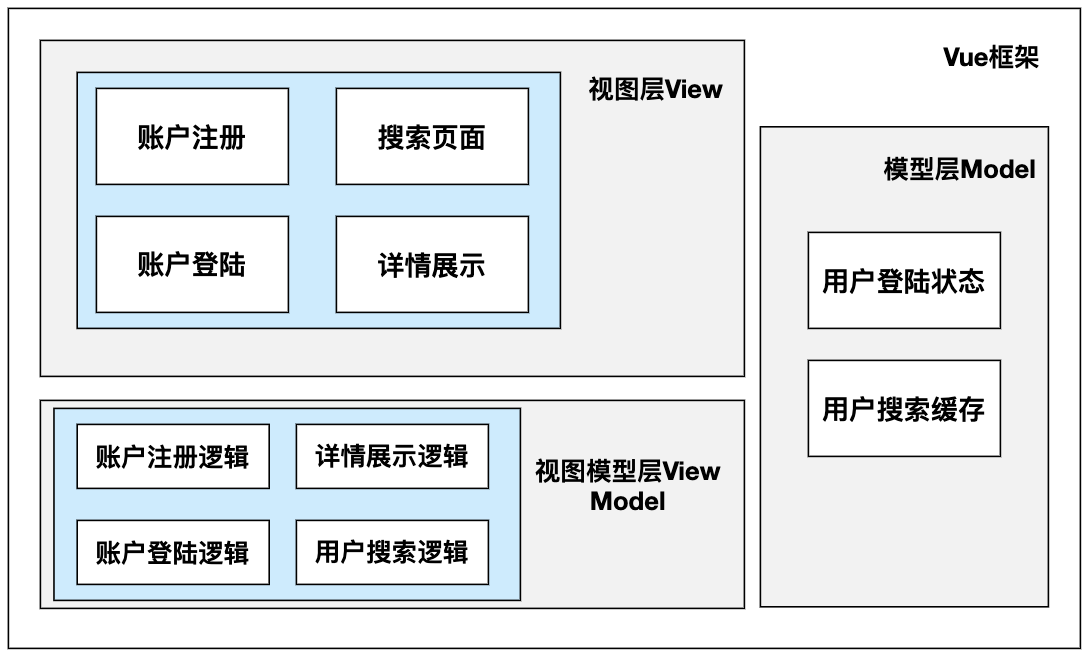
\includegraphics[width=0.95\textwidth]{front_model.png}}
	\caption{前端系统架构图}
	\label{front_model}
\end{figure}

视图层承担着呈现用户界面的职责,它可承载所有的用户交互操作,其主要囊括了开发者的注册与登录界面、代码检索页面、检索结果展示页面、用户个人中心以及项目管理等功能模块,视图层借助Vue的组件化机制达成界面元素的复用以及动态渲染,还支持响应式设计,以此适配不同的终端设备,提升用户体验的流畅程度和一致程度。\par
视图模型层充当着视图层与模型层之间的桥梁,主要负责处理前端业务逻辑,该层实现了账户注册与登录的表单验证以及状态管理、代码搜索请求的构造与发送、检索结果的分页与筛选、项目详情的动态展示等核心功能,视图模型层凭借Vue的响应式数据绑定机制,实时监听用户操作并更新视图状态,以此保证界面与数据可保持同步。该层还负责调用后端API接口,处理异步请求以及错误反馈,保障前后端交互的稳定以及高效。\par
模型层主要用于前端数据的临时存储以及状态管理,系统采用Vuex作为集中式状态管理工具,统一管理用户信息、检索历史、搜索结果以及项目数据等关键状态,模型层凭借对数据变化的监听与响应,实现跨组件的数据共享以及状态同步,避免出现数据冗余和不一致的问题。另外模型层还支持本地缓存机制,比如localStorage或IndexedDB,以此提升用户操作的连续程度和离线体验。\par
为提升系统的可维护性与扩展性,前端架构引入了模块化开发和路由管理,凭借Vue Router实现页面间的动态切换以及权限控制,保证不同用户角色可访问对应功能模块。组件之间凭借事件机制和状态管理进行解耦,方便后续功能迭代以及团队协作开发,总之,本系统前端架构基于Vue MVVM模式,结合组件化、响应式数据绑定和集中式状态管理,构建了一个结构清晰、响应迅速且易于维护的智能代码检索用户界面,为用户提供流畅、高效的交互体验。\par

\subsection{本章小结}
本章对面向多编程语言的代码检索系统展开了较为系统的需求分析与方案设计,涉及从用户需求一直到技术实现等各方面的内容,经过较为细致的用户需求调研,明确了系统要支持多种编程语言以及多种场景下的高效代码检索,以契合开发者和学习者对于代码片段、项目详情以及跨语言查询等多样的需求,同时也突出了安全性和权限管理的意义。基于这些情况,提出了系统的功能需求以及非功能需求,包含强大的检索能力、项目详情展示、VS Code插件集成、高性能响应、可扩展性以及高可用性等关键指标,在方案设计方面,系统采用前后端分离架构,前端依据Vue MVVM模式构建响应式、模块化的交互界面,支持多端一致体验和状态管理,后端则基于微服务架构达成高可用分布式部署,结合服务注册发现、负载均衡和容错机制,保障系统的稳定性以及弹性扩展。数据层借助基于AST的代码结构化预处理,实现多语言代码的统一表示以及高质量索引,提升语义理解和检索精度,总的来说,本章构建了一个架构合理且功能完备的多编程语言智能代码检索系统方案,为后续的系统实现与优化打下了坚实基础,保证系统可高效契合用户多样化需求,提升代码检索水平以及用户体验。\par


\section{面向多编程语言的代码检索系统方案实现}
\subsection{基于AST的编程语言预处理实现}

在本系统的预处理阶段,针对不同编程语言,设计并实现了基于抽象语法树也就是AST的代码结构化处理模块,这个模块主要依靠多种开源AST解析器,像Go语言的go/ast包、Python的ast模块以及Java的JavaParser等,可自动对多语言项目的源代码做语法分析,生成对应的抽象语法树。系统借助统一的接口封装不同语言的解析工具,达成了对多语言代码的统一处理流程,保证了预处理过程的可扩展性与灵活性。\par
\begin{figure}[H]
	\center{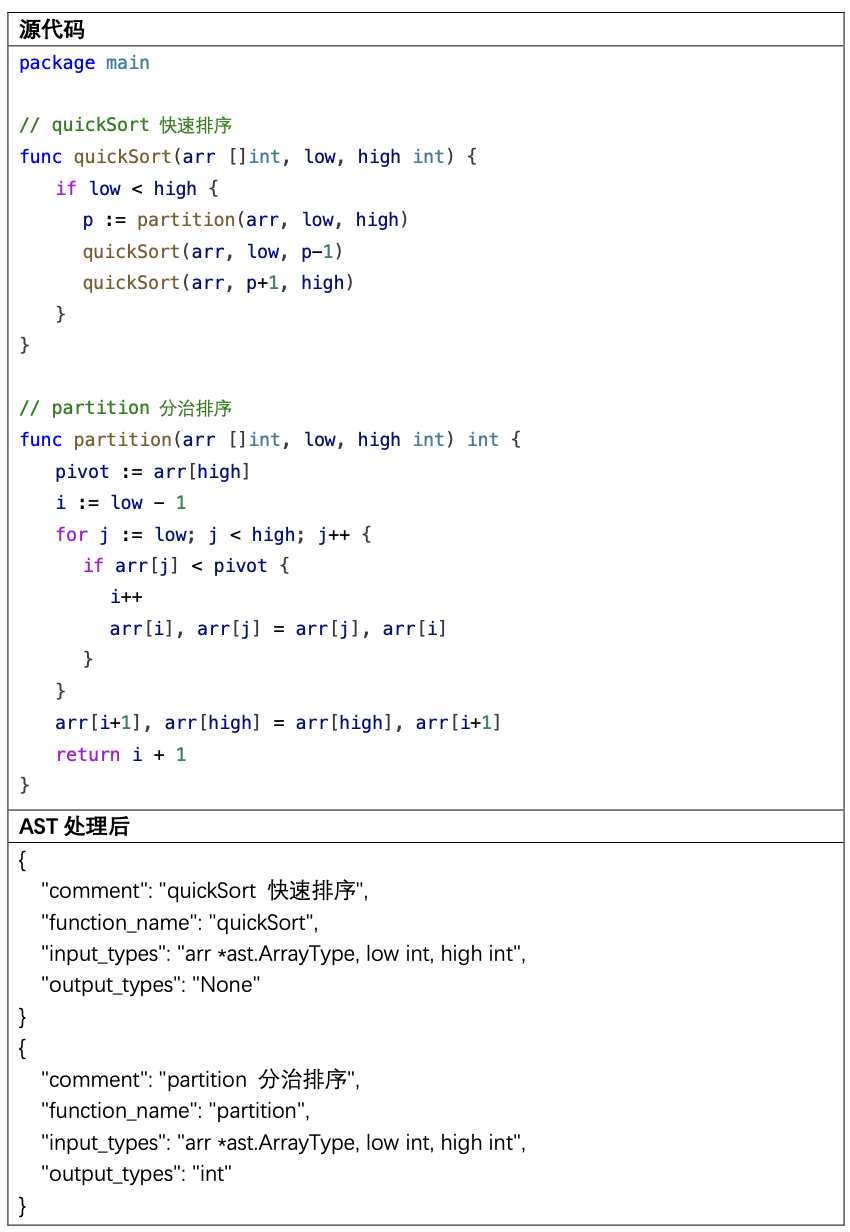
\includegraphics[width=0.95\textwidth]  {ast_example.png}} 
	\caption{AST处理示例图}
	\label{ast_example}
\end{figure}
系统先是对收集到的代码仓库进行遍历,针对每个文件调用对应语言的AST解析器,自动生成完整的语法树结构,之后系统对生成的AST进行深度遍历,筛选出与核心业务逻辑有关的代码节点,自动去除注释、单元测试代码以及无实际功能的辅助代码片段。这一步骤有效提高了数据集的纯净度,避免了无关信息对后续检索模型的干扰,为了提高数据的一致性以及跨语言对齐能力,系统对保留的功能函数进行了结构化处理,覆盖统一节点类型的命名规范,以及对变量名和函数标识符的标准化处理,减少了不同语言间的命名差异对检索效果的影响。\par
如图\ref{ast_example}所示,系统以一段Go语言实现的快速排序代码为例,经过AST处理后,去掉了具体的递归实现细节,只保留了函数名、注释信息以及方法的输入输出类型等关键信息,极大地规范了代码的存储格式,这种处理保证了代码结构的完整性,也为后续的语义分析和跨语言检索提供了高质量的输入数据。借助该预处理模块,系统可有效地把多语言源代码转化为统一且结构化的中间表示,提升了代码检索的准确性和效率,整体而言,基于AST的预处理实现为多编程语言代码检索系统奠定了坚实基础,保证了后续检索服务可在多语言环境下高效运行。\par


\subsection{基于微服务的高可用后台分布式技术实现}
\subsubsection{微服务系统中的统一接入与安全网关服务}
在基于微服务的分布式系统里,服务网关是保障整体服务安全、有可扩展性以及拥有高可用性的核心基础设施之一,服务网关指的是在分布式微服务系统当中,作为所有外部请求的统一入口,承担着流量调度、统一鉴权、安全防护、协议转换等多项关键任务,和传统单体系统的直接访问模式不一样,服务网关借助集中管理和智能路由,有效隐藏了后端服务的复杂性,提高了系统的安全性、灵活性以及运维效率。在面向多编程语言的代码检索系统中,网关机制承担着请求分发和安全防护的基本职责,还需要适应多语言、多协议以及高并发的复杂业务场景,以此保障系统整体的稳定运行以及高效服务能力。\par

\begin{figure}[H]
	\center{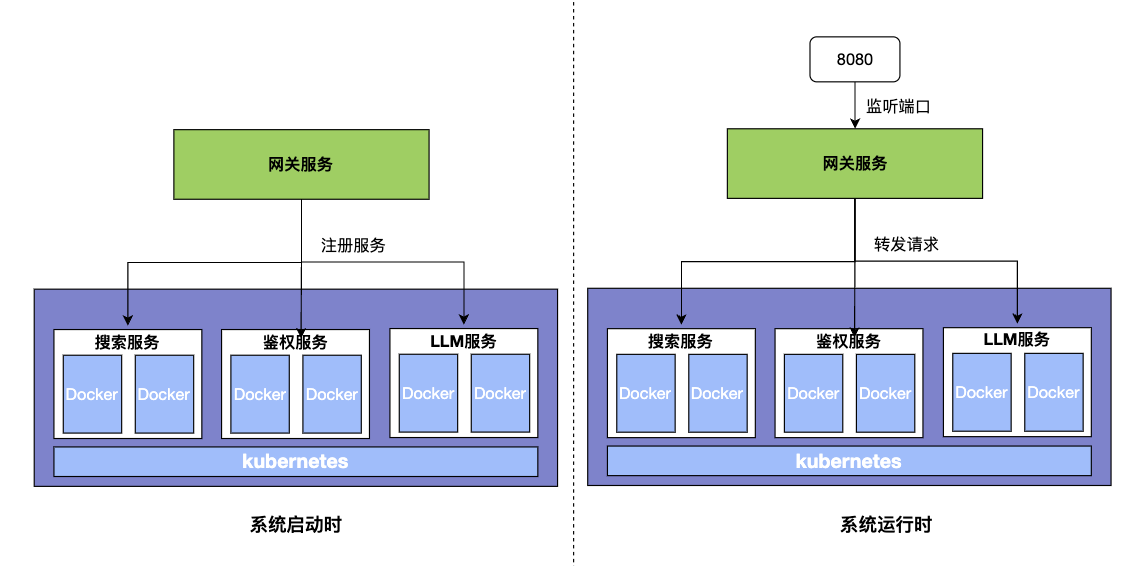
\includegraphics[width=0.95\textwidth]  {gateway.png}} 
	\caption{网关工作原理图}
	\label{gateway}
\end{figure}


在面向多编程语言的代码检索系统中,网关服务基于Gin框架,基本上实现了服务的统一注册、均衡路由以及服务鉴权等功能。图\ref{gateway}是本服务的网关服务的简单工作原理图示例,网关的工作过程分成服务启动时和服务运行时两个阶段,服务启动时,网关会向鉴权服务、搜索服务以及大语言模型服务发送探活请求,保证系统内所有服务都可正常连接,服务运行时,网关服务监听服务器的特定端口。在本系统中,网关监听8080端口,所有的请求经过网关集成的多种负载均衡策略中的一种,依据实时流量和服务健康状态,智能分发至后端对应的微服务实例,对于所有的请求,都要经过鉴权服务鉴权,保证请求访问的权限在安全控制范围内。\par
\subsubsection{微服务系统中的统一身份认证与安全鉴权服务}
在现代微服务系统里边,统一身份认证跟安全鉴权机制属于保障系统安全性、数据完整性以及用户隐私的核心基础设施,所说的鉴权服务,是在多服务协同的分布式系统当中,专门负责用户身份验证、权限校验以及会话管理的独立服务模块,跟传统单体系统里嵌入式的认证方式不一样,分布式鉴权系统借助集中式管理和标准化接口,有效提高了系统的安全性、可扩展性以及运维效率,而且大多时候依赖分布式数据库解决统一路由问题。在面向多编程语言的代码检索系统中,鉴权服务承担着用户注册、登录以及会话管理的基本职责,还得适应高并发环境下的复杂业务场景,为系统的安全运行和用户体验提供坚实保障。\par
\begin{figure}[H]
	\center{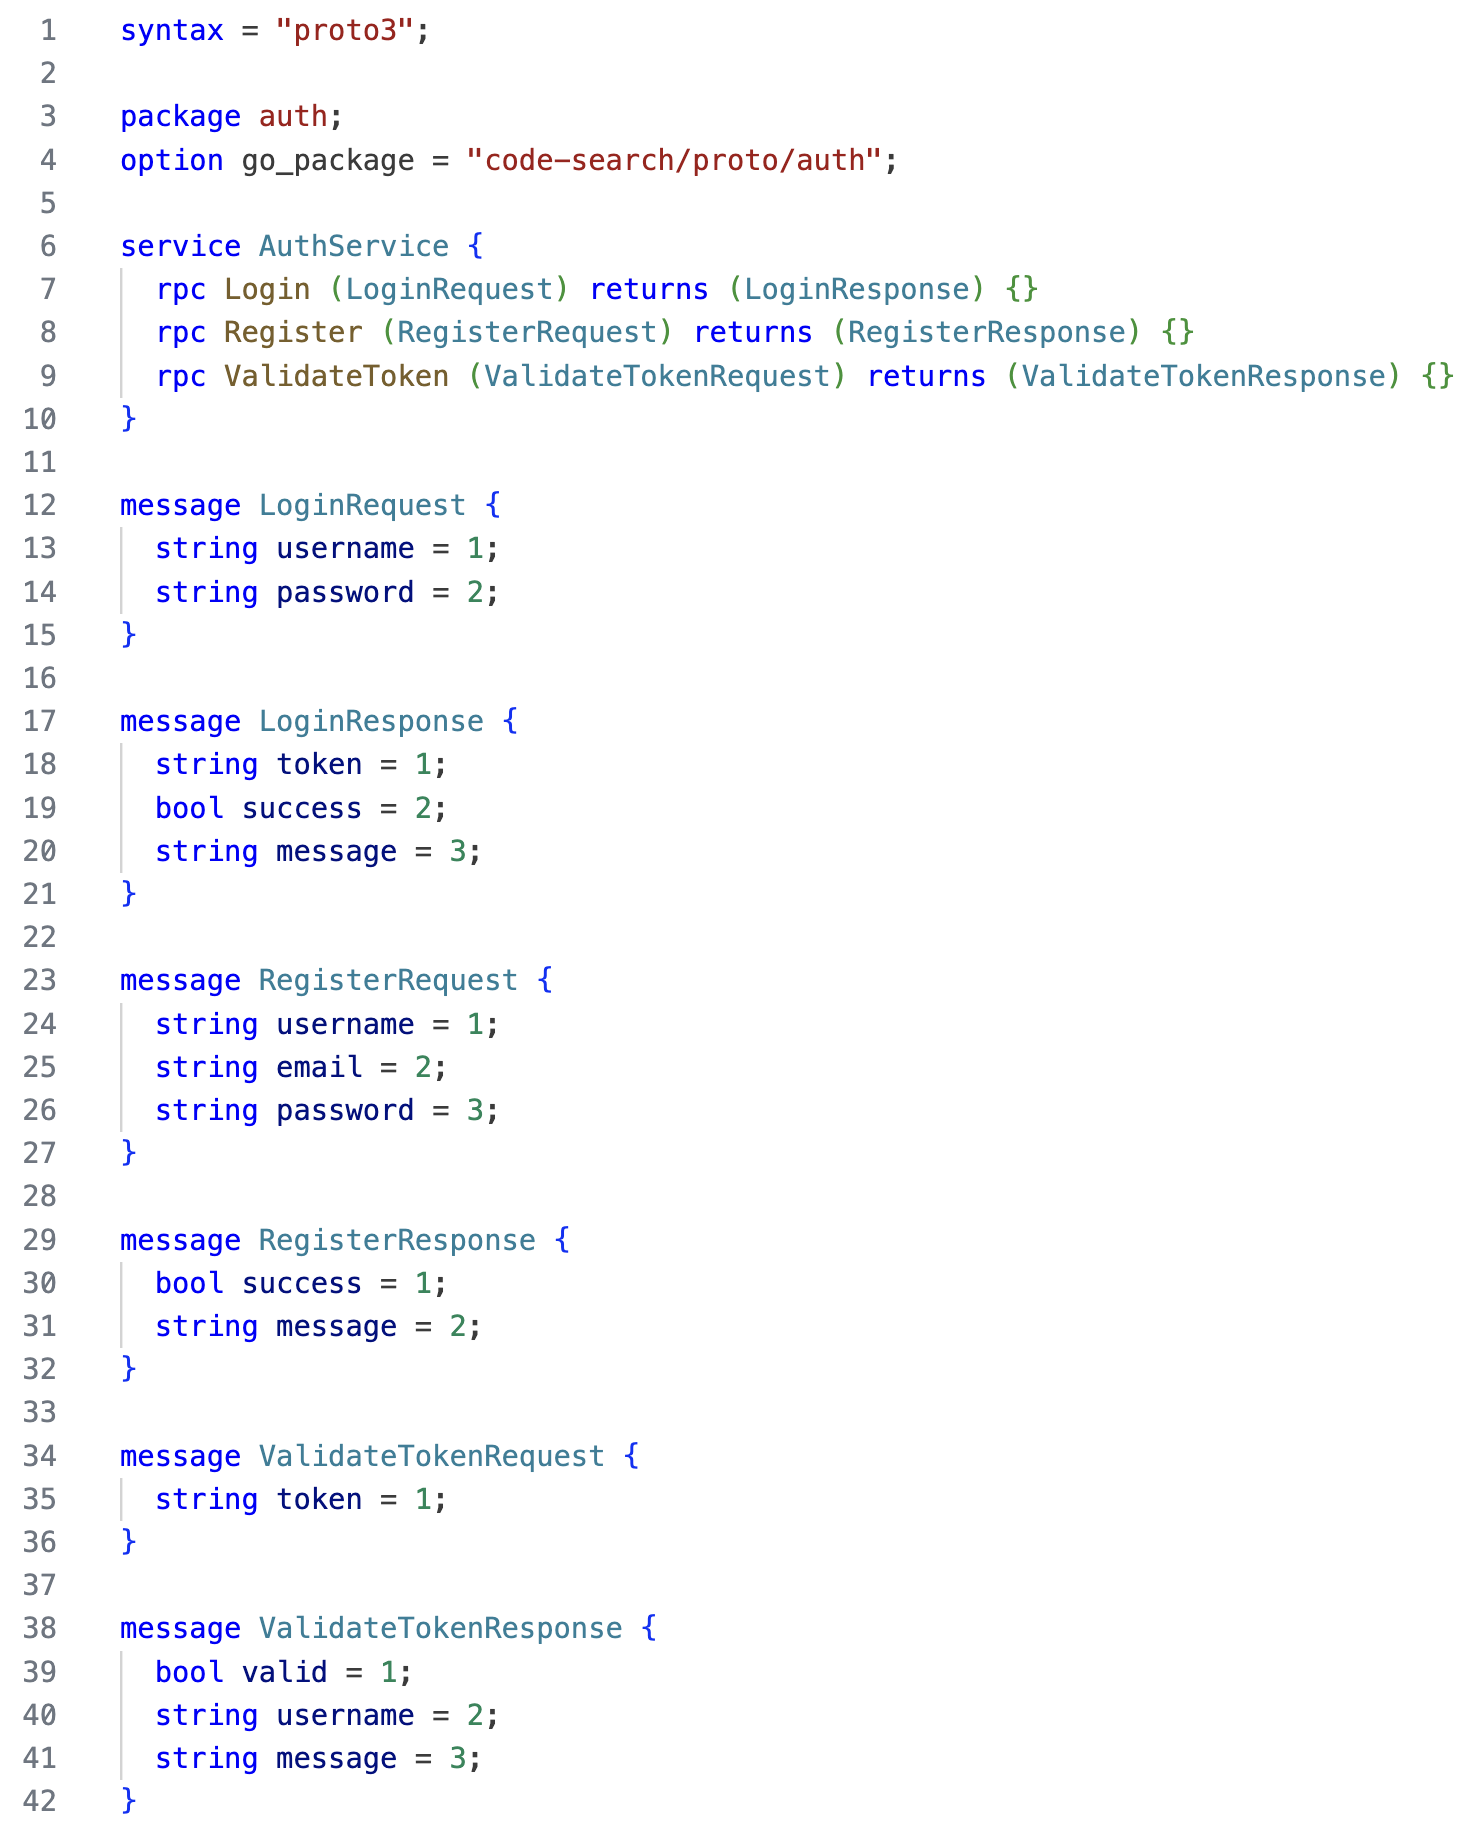
\includegraphics[width=0.95\textwidth]  {proto.png}} 
	\caption{鉴权服务协议}
	\label{auth}
\end{figure}
本系统的统一身份认证与安全鉴权机制依靠gRPC高性能通信框架来实现,采用如图\ref{auth}所示的标准化的proto协议定义服务接口,保证各微服务间的高效互操作与安全通信。整体流程包含用户注册、登录认证以及会话状态校验等核心环节,如图\ref{auth_flow}所示,具体有以下三个阶段:\par
\begin{figure}[H]
	\center{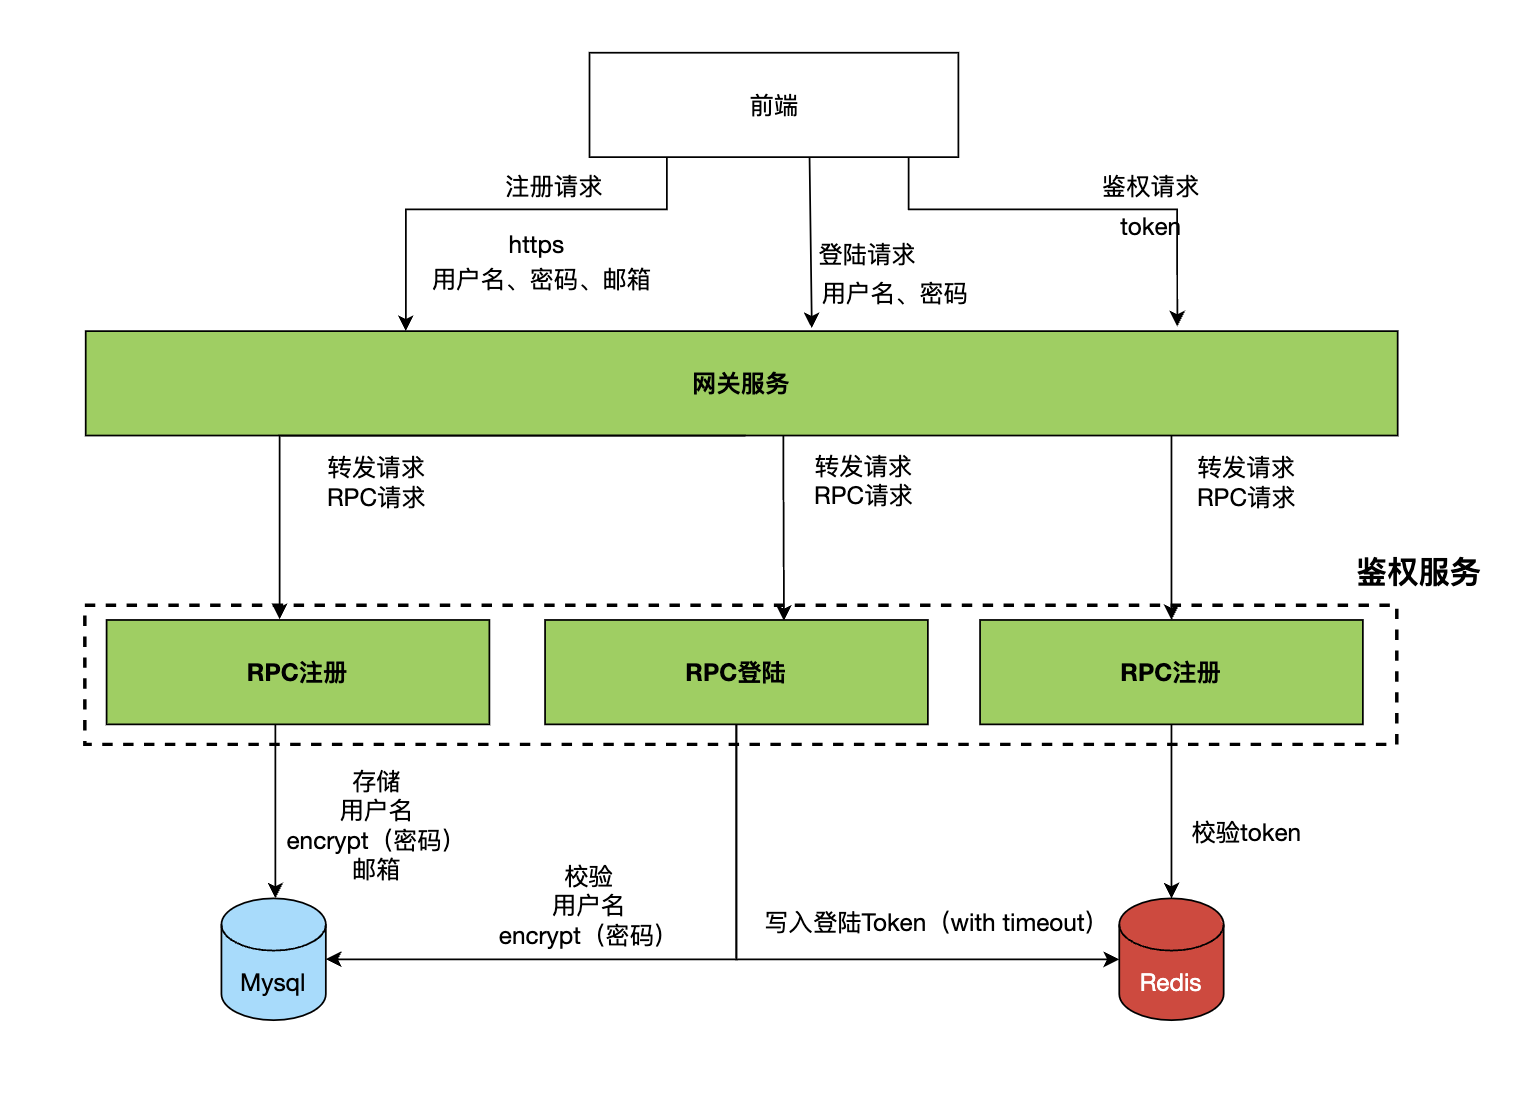
\includegraphics[width=0.95\textwidth]{auth.png}}
	\caption{统一身份认证与鉴权服务工作原理}
	\label{auth_flow}
\end{figure}
第一阶段是用户注册与身份信息安全存储,用户借助前端界面提交用户名、邮箱以及密码等注册信息,所有注册请求都依靠HTTPS协议加密传输到服务网关,以此防止敏感数据在传输过程中被窃取。服务网关对请求进行初步校验后,把它转发到鉴权服务的注册接口,为了保障用户密码安全,系统采用哈希加密算法对密码进行不可逆处理,最后将加密后的密码存储在数据库中,即便数据库遭受攻击,用户的原始密码信息也没办法被直接获取,有效提升了系统的抗攻击能力,用户注册信息表如表\ref{usertable}所示,其中id字段作为用户的唯一标识符,由系统使用雪花算法自动生成。雪花算法是一种高效且被广泛认可的ID生成方案,可在本项目的用户基数和并发量下充分保证ID的唯一性,用户名、电子邮件以及密码字段用于用户的注册和认证过程,而且密码在存储前都经过哈希加密处理,在数据传输和存储环节保障了用户信息的安全性。\par
\begin{table}[H]
	\centering
	\caption{用户信息表(code\_search\_user)}
	\small
	\begin{tabular}{c c c c}
		\toprule
		列名 & 数据类型 & 主键 & 注释\\
		\midrule
		id & bigint & 是 & 用户ID(通过雪花算法自动生成)\\
		username & varchar(255) & 否 & 用户名\\
		email & varchar(255) & 否 & 用户电子邮件地址\\
		password & varchar(255) & 否 & 用户密码(采用哈希加密存储)\\
		\bottomrule
	\end{tabular}
	\label{usertable}
\end{table}
第二阶段是用户登录以及会话令牌分发,用户输入用户名与密码来发起登录请求,系统收到请求后,会针对用户提交的凭证开展哈希校验工作,认证凭借以后,鉴权服务给用户生成唯一的会话 Token,并且把这个 Token 安全存放在分布式 Redis 集群里,从这之后,用户访问系统各项服务时,都要携带这个 Token 来证明自身身份的合法性。Token 机制对提升系统安全性有帮助,同时也方便实现分布式环境下的无状态会话管理。\par
第三阶段是会话状态检测以及权限校验,每次用户发起请求时,都要在请求头中携带有效的 Token,服务网关收到请求后,会先把 Token 转发到鉴权服务去进行有效性校验。鉴权服务凭借验证 Token 的合法性以及它在 Redis 集群中的存在情况或者有没有超时淘汰,来判断用户会话是否有效,要是校验依靠,网关就会放行请求并转发到目标微服务,要是校验失败,就拒绝请求并返回相应的错误信息,这个机制能有效防止未授权访问和会话劫持等安全风险,保障系统的整体安全性与稳定性。\par
\subsubsection{基于高性能分布式查询引擎的代码查询服务}

在面向多编程语言的代码检索系统里,基于分布式的高性能查询引擎属于实现高效且精准检索体验的关键功能模块,这项服务是在前期对AST预处理的基础上开展的,同时依赖LLM去深入理解和重写用户的查询意图,再结合Elasticsearch高性能检索引擎,最终达成了高效的代码查询以及结果排序。本章节会介绍查询服务的整体任务流程,还会着重讲一下高性能分布式查询引擎Elasticsearch在本项目中的具体运用情况。\par
该服务借助gRPC高性能远程过程调用框架得以实现,采用protobuf协议来定义标准化的服务接口,协议如图\ref{search_proto}所示。\par
\begin{figure}[H]
	\center{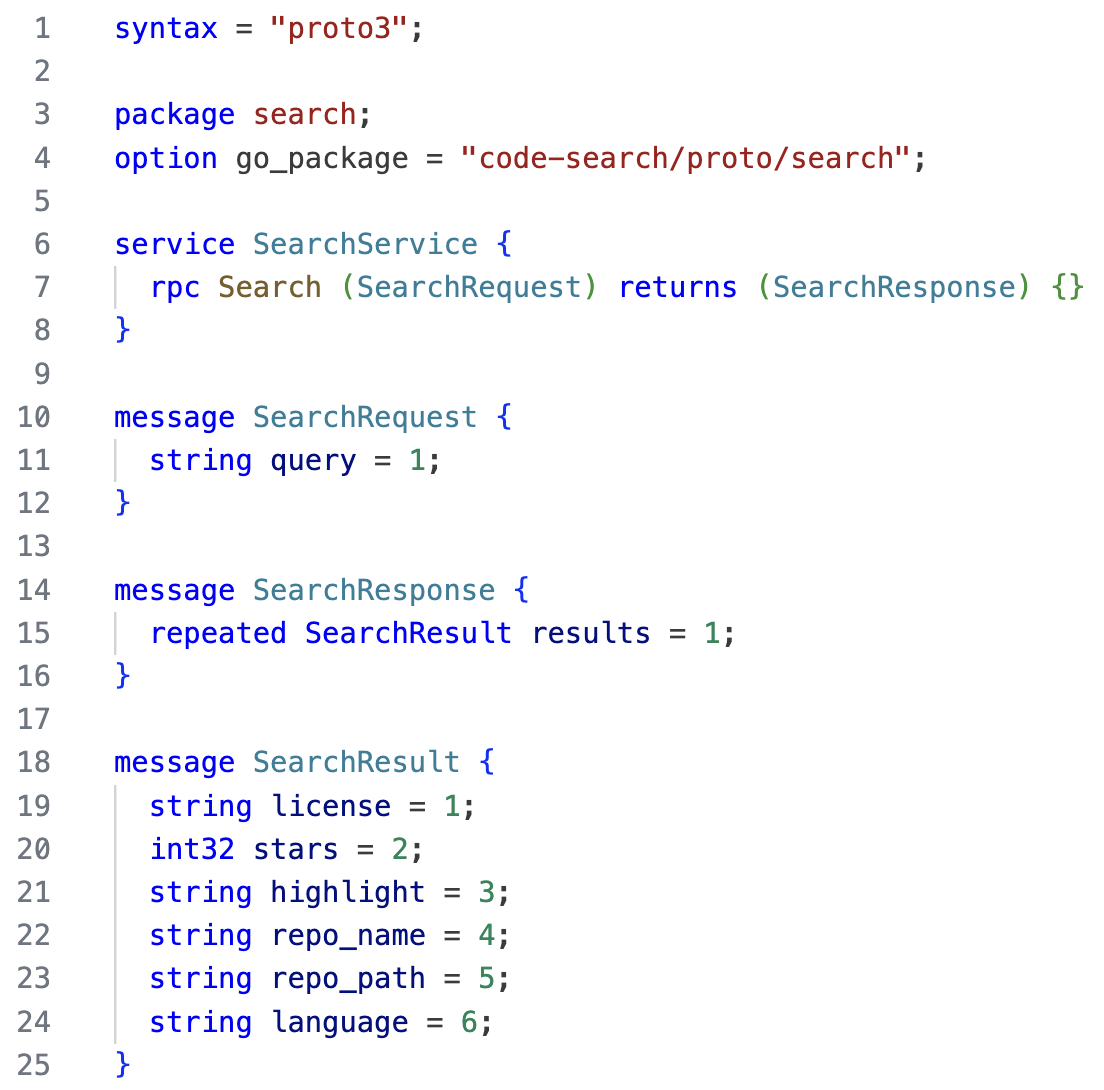
\includegraphics[width=0.95\textwidth]{search_proto.png}}
	\caption{智能搜索服务协议}
	\label{search_proto}
\end{figure}
用户的检索请求凭借Search接口来提交,SearchRequest与SearchResponse分别对请求与响应的数据结构做了定义,其中SearchResponse结构体含有SearchResult列表,用来承载多样化的检索结果,能支持多语言、多协议以及多维度的代码查询需求。系统整体的用户搜索流程如图\ref{timeline}所示,用户经过鉴权之后提交检索请求,系统会把用户的原始查询语句发送到模型侧,模型对用户查询意图进行深入理解并做专业化改写,然后将优化后的检索词返回给查询系统,系统接着把经过大模型处理的检索请求发送到底层数据库,数据库返回查询结果,最后由系统进行可视化展示。\par

\begin{figure}[H]
	\center{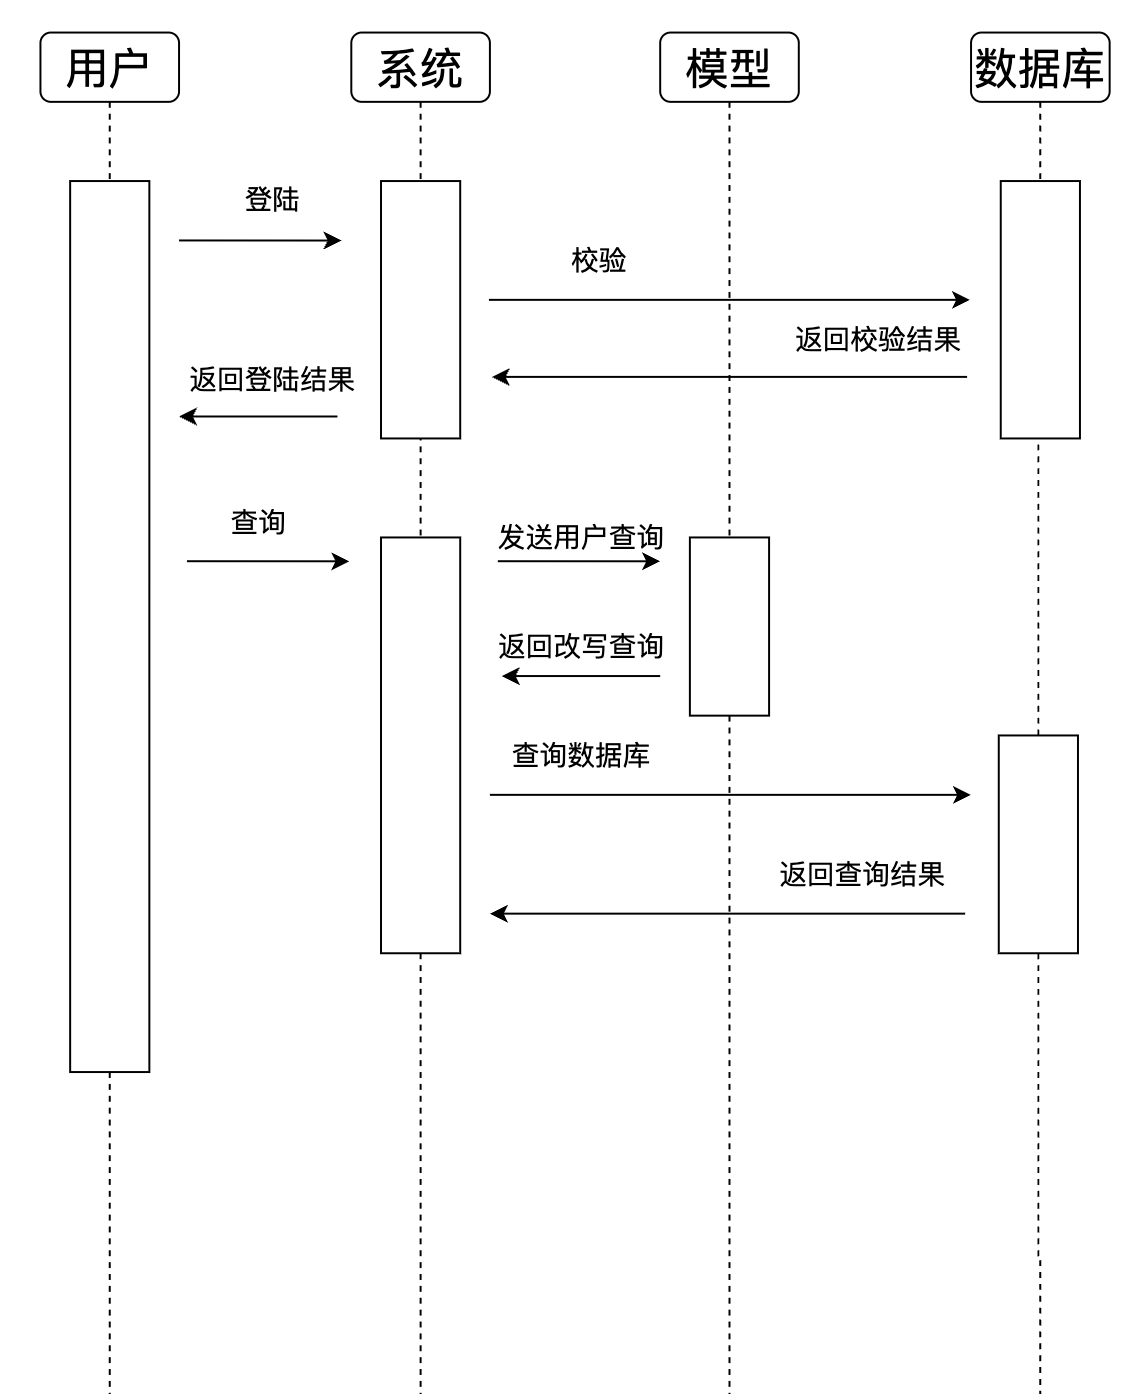
\includegraphics[width=0.4\textwidth]{timeline.png}}
	\caption{用户搜索时序图}
	\label{timeline}
\end{figure}
Elasticsearch作为底层分布式检索引擎,负责代码数据的高效存储、索引以及查询任务,为契合多语言、多协议、多维度的检索需求,系统在Elasticsearch里为代码数据设计了结构化的Mapping,如表\ref{esmapping}所示。
\begin{table}[H]
	\centering
	\caption{索引code的映射结构}
	\label{tab:code_mapping}
	\small
	\begin{tabular}{c c c}
		\toprule
		字段名 & 数据类型 & 描述 \\
		\midrule
		content & text & 代码内容(文本类型) \\
		file\_name & keyword & 文件名(关键字类型) \\
		repo\_name & keyword & 文件所属项目名(关键字类型)\\
		lang & keyword & 编程语言(关键字类型) \\
		lic & keyword & 许可证类型(关键字类型) \\
		stars & integer & 星标数量(整数类型) \\
		\bottomrule
	\end{tabular}
	\label{esmapping}
\end{table}
在这个Mapping结构里,content字段是text类型,它支持分词以及全文检索,能针对代码内容开展高效的语义匹配与相关性排序,file\_name和repo\_name字段属于keyword类型,有利于对特定文件或者项目实施精确过滤以及聚合统计,同时也便于在搜索结果里展示文件和项目的详细信息。lang字段用于标明代码所采用的编程语言,lic字段记录代码的开源协议类型,这两个字段都是keyword类型,可支撑高效的条件过滤以及多维度聚合分析,stars字段记录项目的星标数量,是integer类型,便于对检索结果进行数值排序以及统计分析,比如优先展示高星项目或者实现项目热度排行。依据上述Mapping结构,系统可灵活地支持多维度的检索需求,在实际查询流程中,服务端会依照LLM生成的结构化检索指令,把用户的查询意图映射到Elasticsearch的复合查询语句中,以此提升查询的联想能力和准确性。\par
\subsection{基于提示词工程的查询上下文增强技术}
为达成查询语句的上下文提高功能,本文构思了一种多层次的提示词模板,其基本结构呈现于图\ref{prompt1},此结构围绕“任务-思维链-结构化输出”展开,对用户的自然语言查询进行系统地剖析与重塑,提示词先引领大语言模型逐个分析语言、协议、技术这三个维度,能捕捉用户的明显需求,又可挖掘潜在的上下文信息与技术细节。模型要判断查询是否针对特定编程语言,依此设定检索范围,接着,识别用户对开源协议的潜在需求,保证检索结果的合规性,深入剖析与查询相关的API、库、框架以及典型技术关键词,提高检索的专业性与覆盖面,在输出格式方面,提示词模板运用<Think>标签对模型的推理过程进行显式分层,让模型分别阐述对每一维度的分析思路,提高推理的可解释性与透明度。系统把分析结果以结构化的JSON格式输出,明确标注检索语言、协议要求以及技术关键词,为后续的代码检索模块提供高质量且可直接执行的查询指令。\par
\begin{figure}[H]
	\center{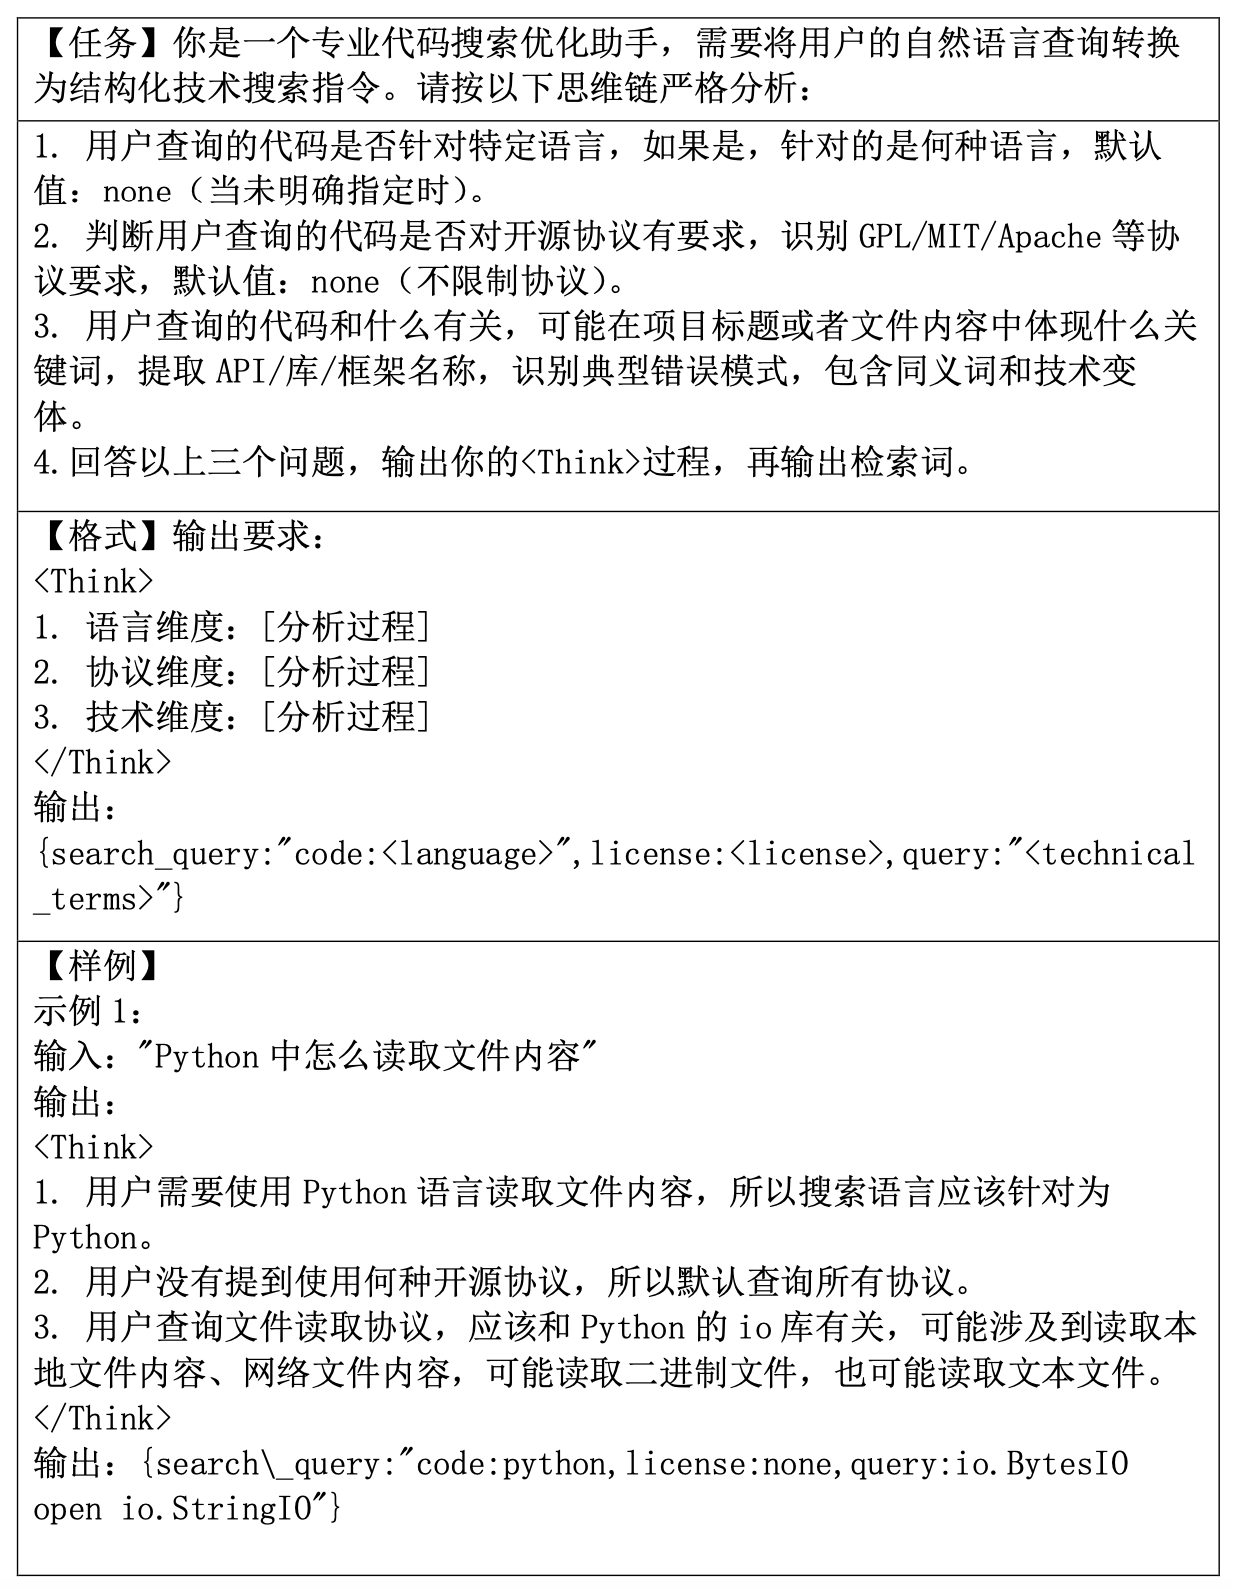
\includegraphics[width=0.95\textwidth]  {prompt1.png}} 
	\caption{提示词结构}
	\label{prompt1}
\end{figure}
\begin{figure}[H]
	\center{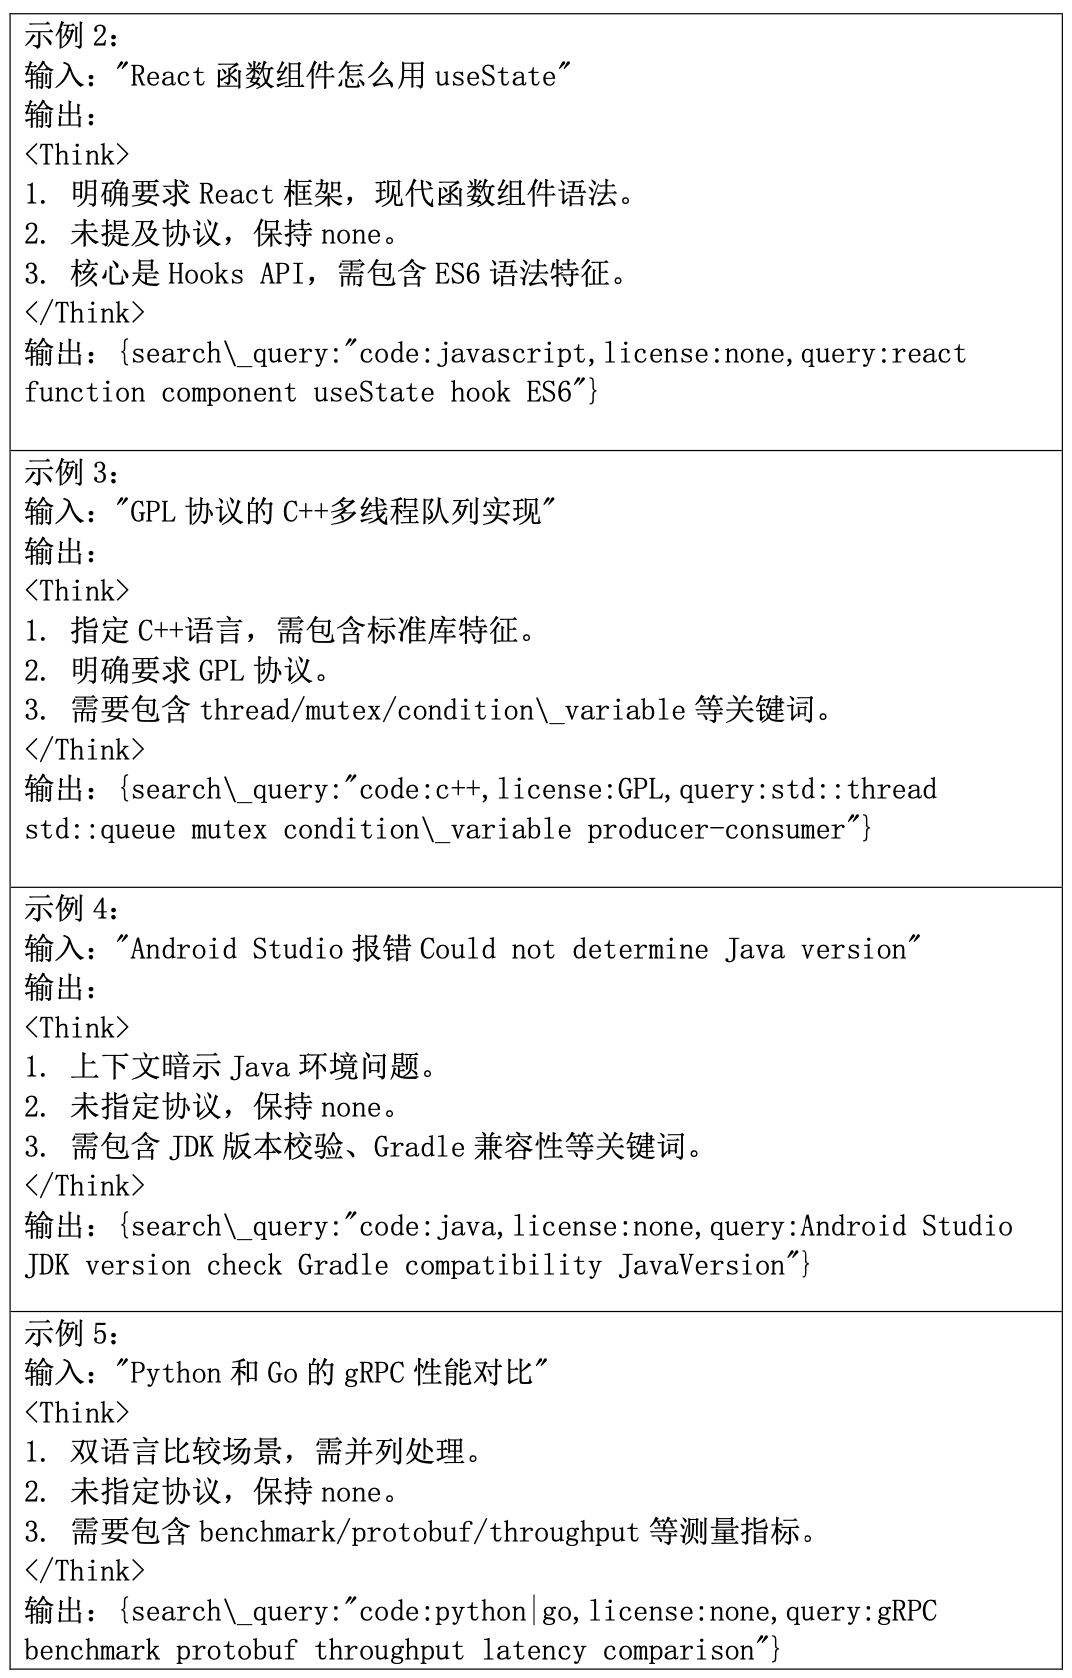
\includegraphics[width=0.95\textwidth]  {prompt2.png}} 
	\caption{提示词结构}
	\label{prompt2}
\end{figure}
另外,如图\ref{prompt2}所示,本文引入了few-shot示例驱动的提示词工程方法,借助在提示词模板中配备多样的输入输出示例,涉及单语言检索、框架API查询、协议限定、错误诊断以及多语言对比等典型场景,模型可更有效地学习如何把复杂、模糊的自然语言需求转化为精确、结构化的检索表达。few-shot示例为模型提供了清晰的任务范式与推理参考,还提升了模型在多编程语言代码检索任务中的理解能力与检索准确率,凭借这种“任务-思维链-结构化输出”的提示词工程方法,系统可有效适应多样化的用户需求,提升整体检索性能与用户体验。\par
\subsection{智能代码检索系统前端界面设计实现}
系统有凭借VS Code插件来开展代码检索的功能,这极大地提升了用户使用时的便捷程度,该插件是依靠VS Code所提供的texttt{vscode.WebviewViewProvider}接口进行开发的,可把前端Web页面毫无缝隙地集成到VS Code左侧的Tab栏当中。用户只要点击Tab栏上的按钮,便可进入到代码搜索界面,去体验和Web端一样的检索以及结果展示功能,插件的界面如图\ref{vscode}所示,插件内部运用的是和Web端一样的Vue组件以及状态管理方案,以此来保证功能和交互体验的一致性,另外插件借助VS Code的消息传递机制来实现与扩展后台的通信,支持异步请求以及结果回传,保障检索过程的流畅与稳定。
\begin{figure}[H]
	\center{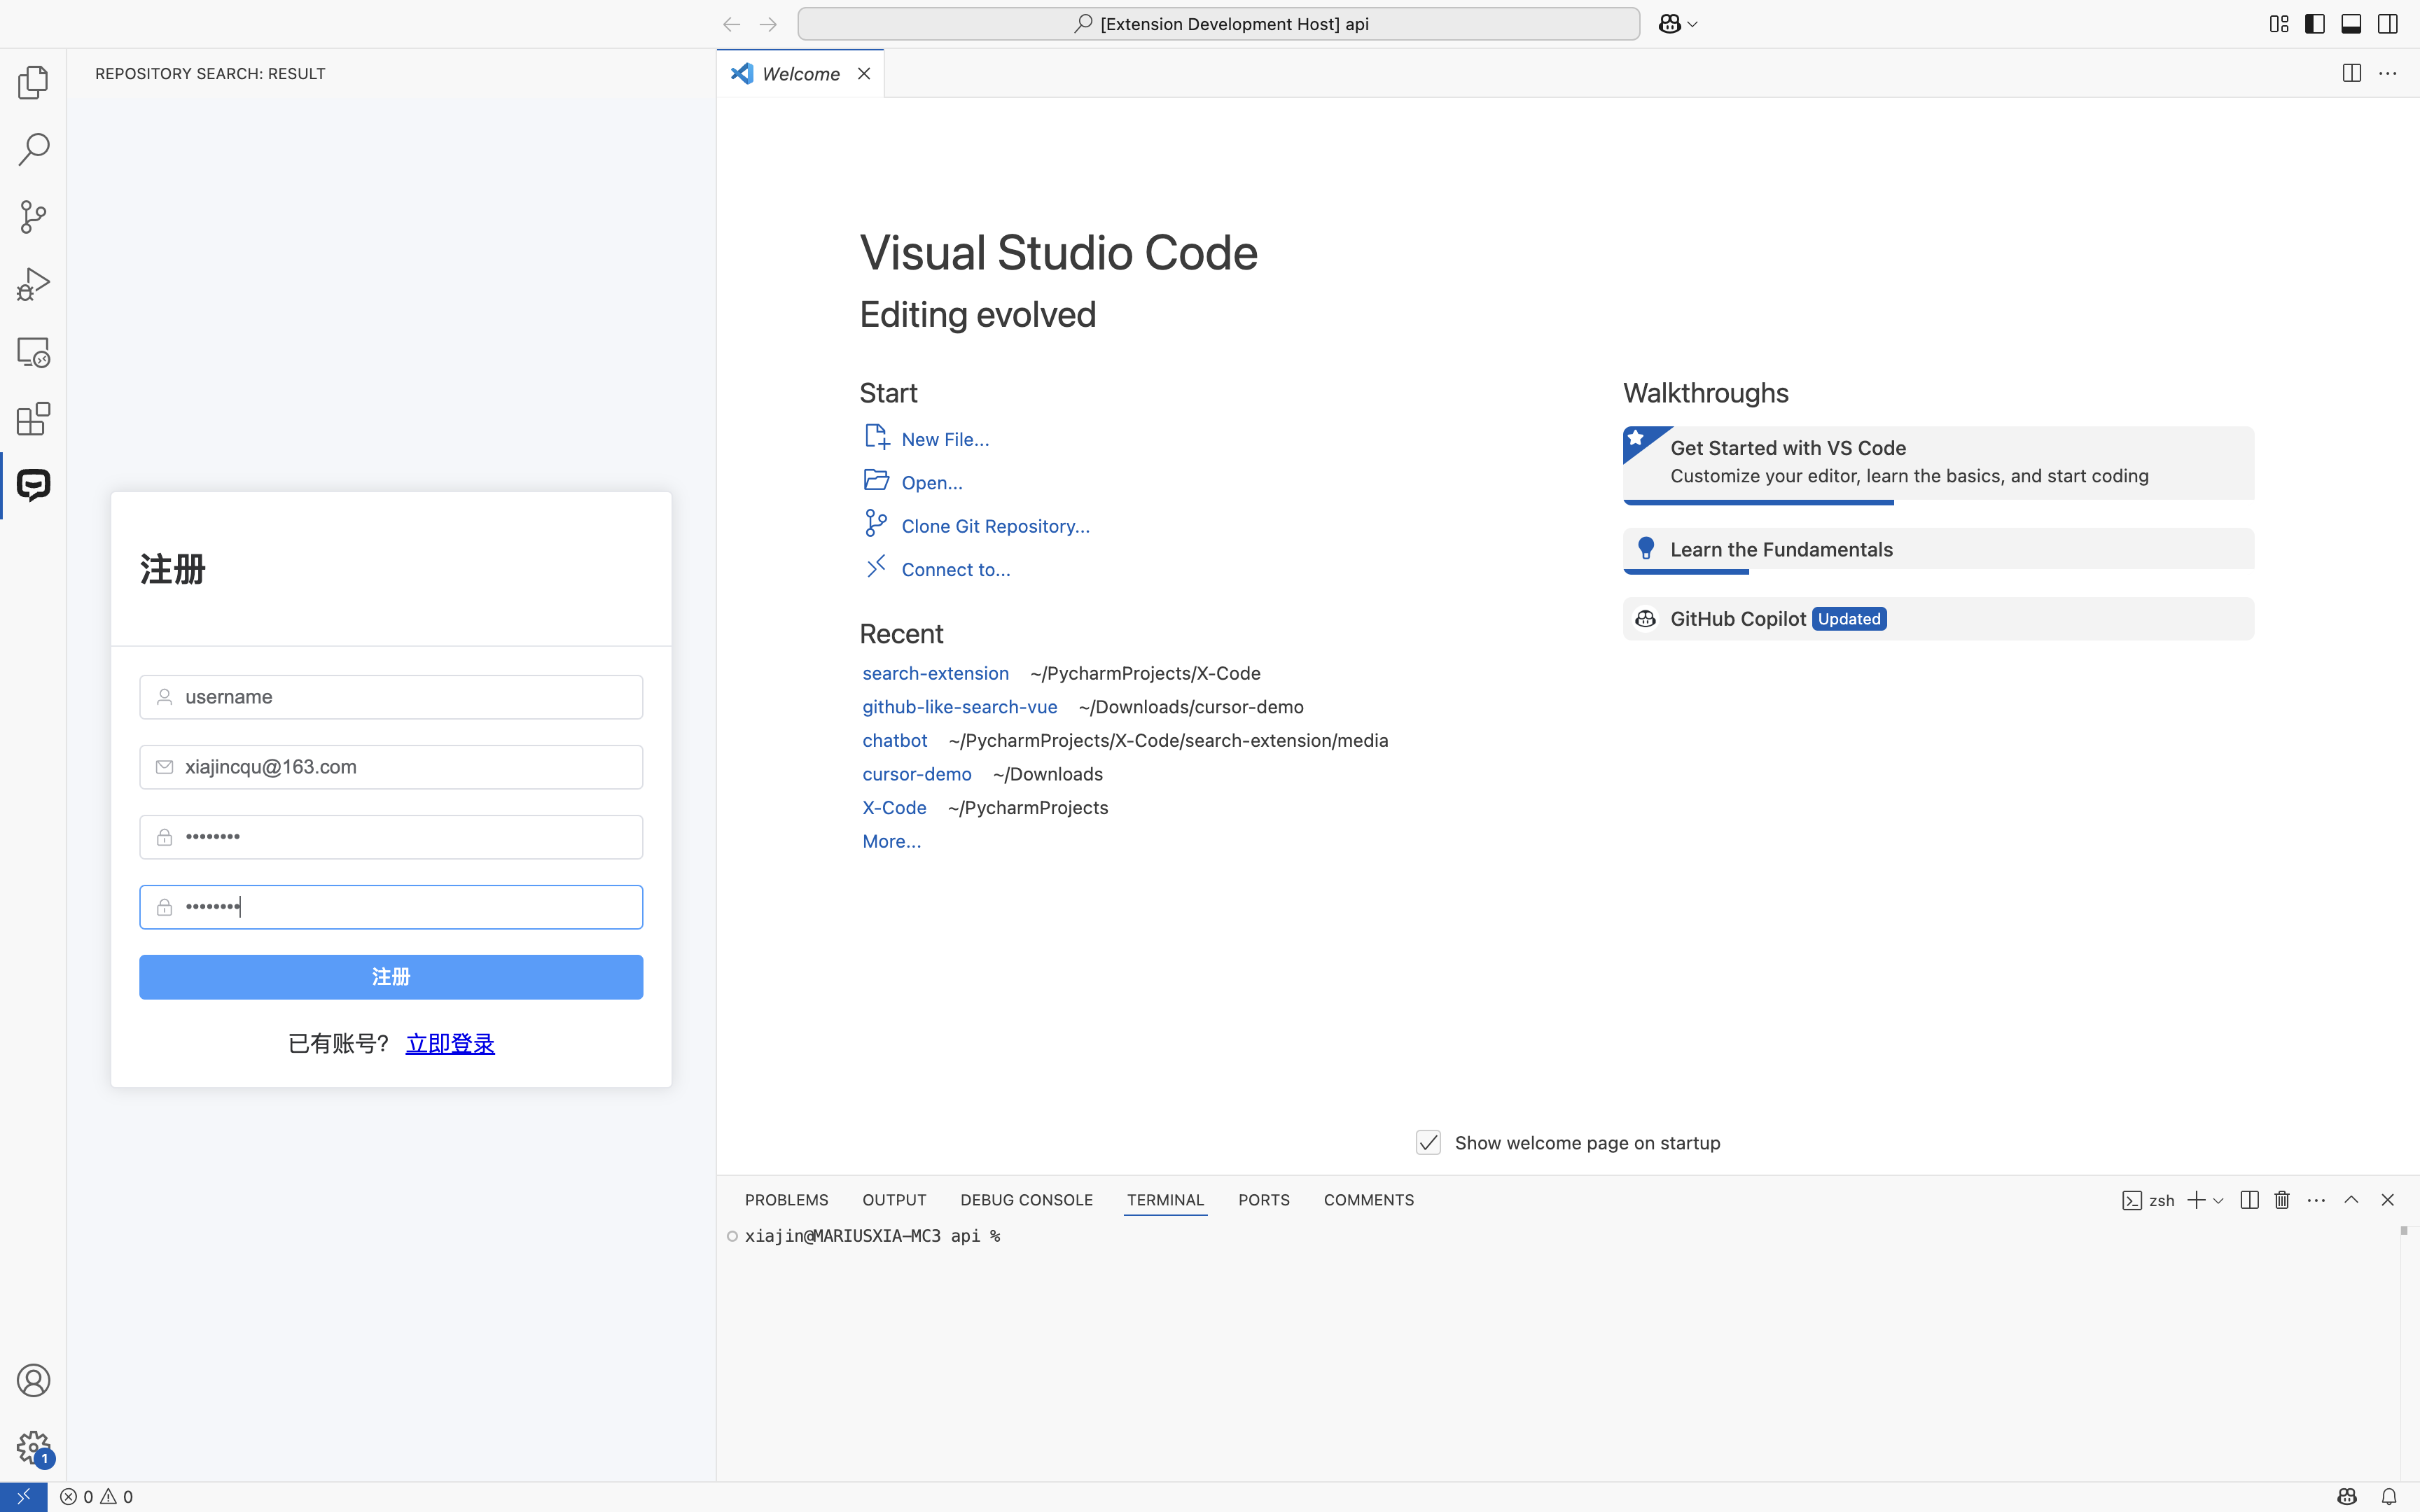
\includegraphics[width=0.95\textwidth]{register.png}}
	\caption{VS Code插件页面}
	\label{vscode}
\end{figure}


在登录界面,如图\ref{logincheck}以及图\ref{loginpage}呈现的那样,系统达成了账号密码输入的前端校验工作,以此防止空表单被提交,提升系统的安全性以及用户体验,输入框绑定了实时校验规则,当用户进行输入时可即时反馈格式错误或者缺失信息。用户信息在前端借助加密算法完成加密处理后,安全地传输至后端进行身份校验,以此保障数据传输的安全,当登录失败时,界面会给出清晰明确的错误提示,帮助用户快速定位问题所在。
\begin{figure}[H]
	\center{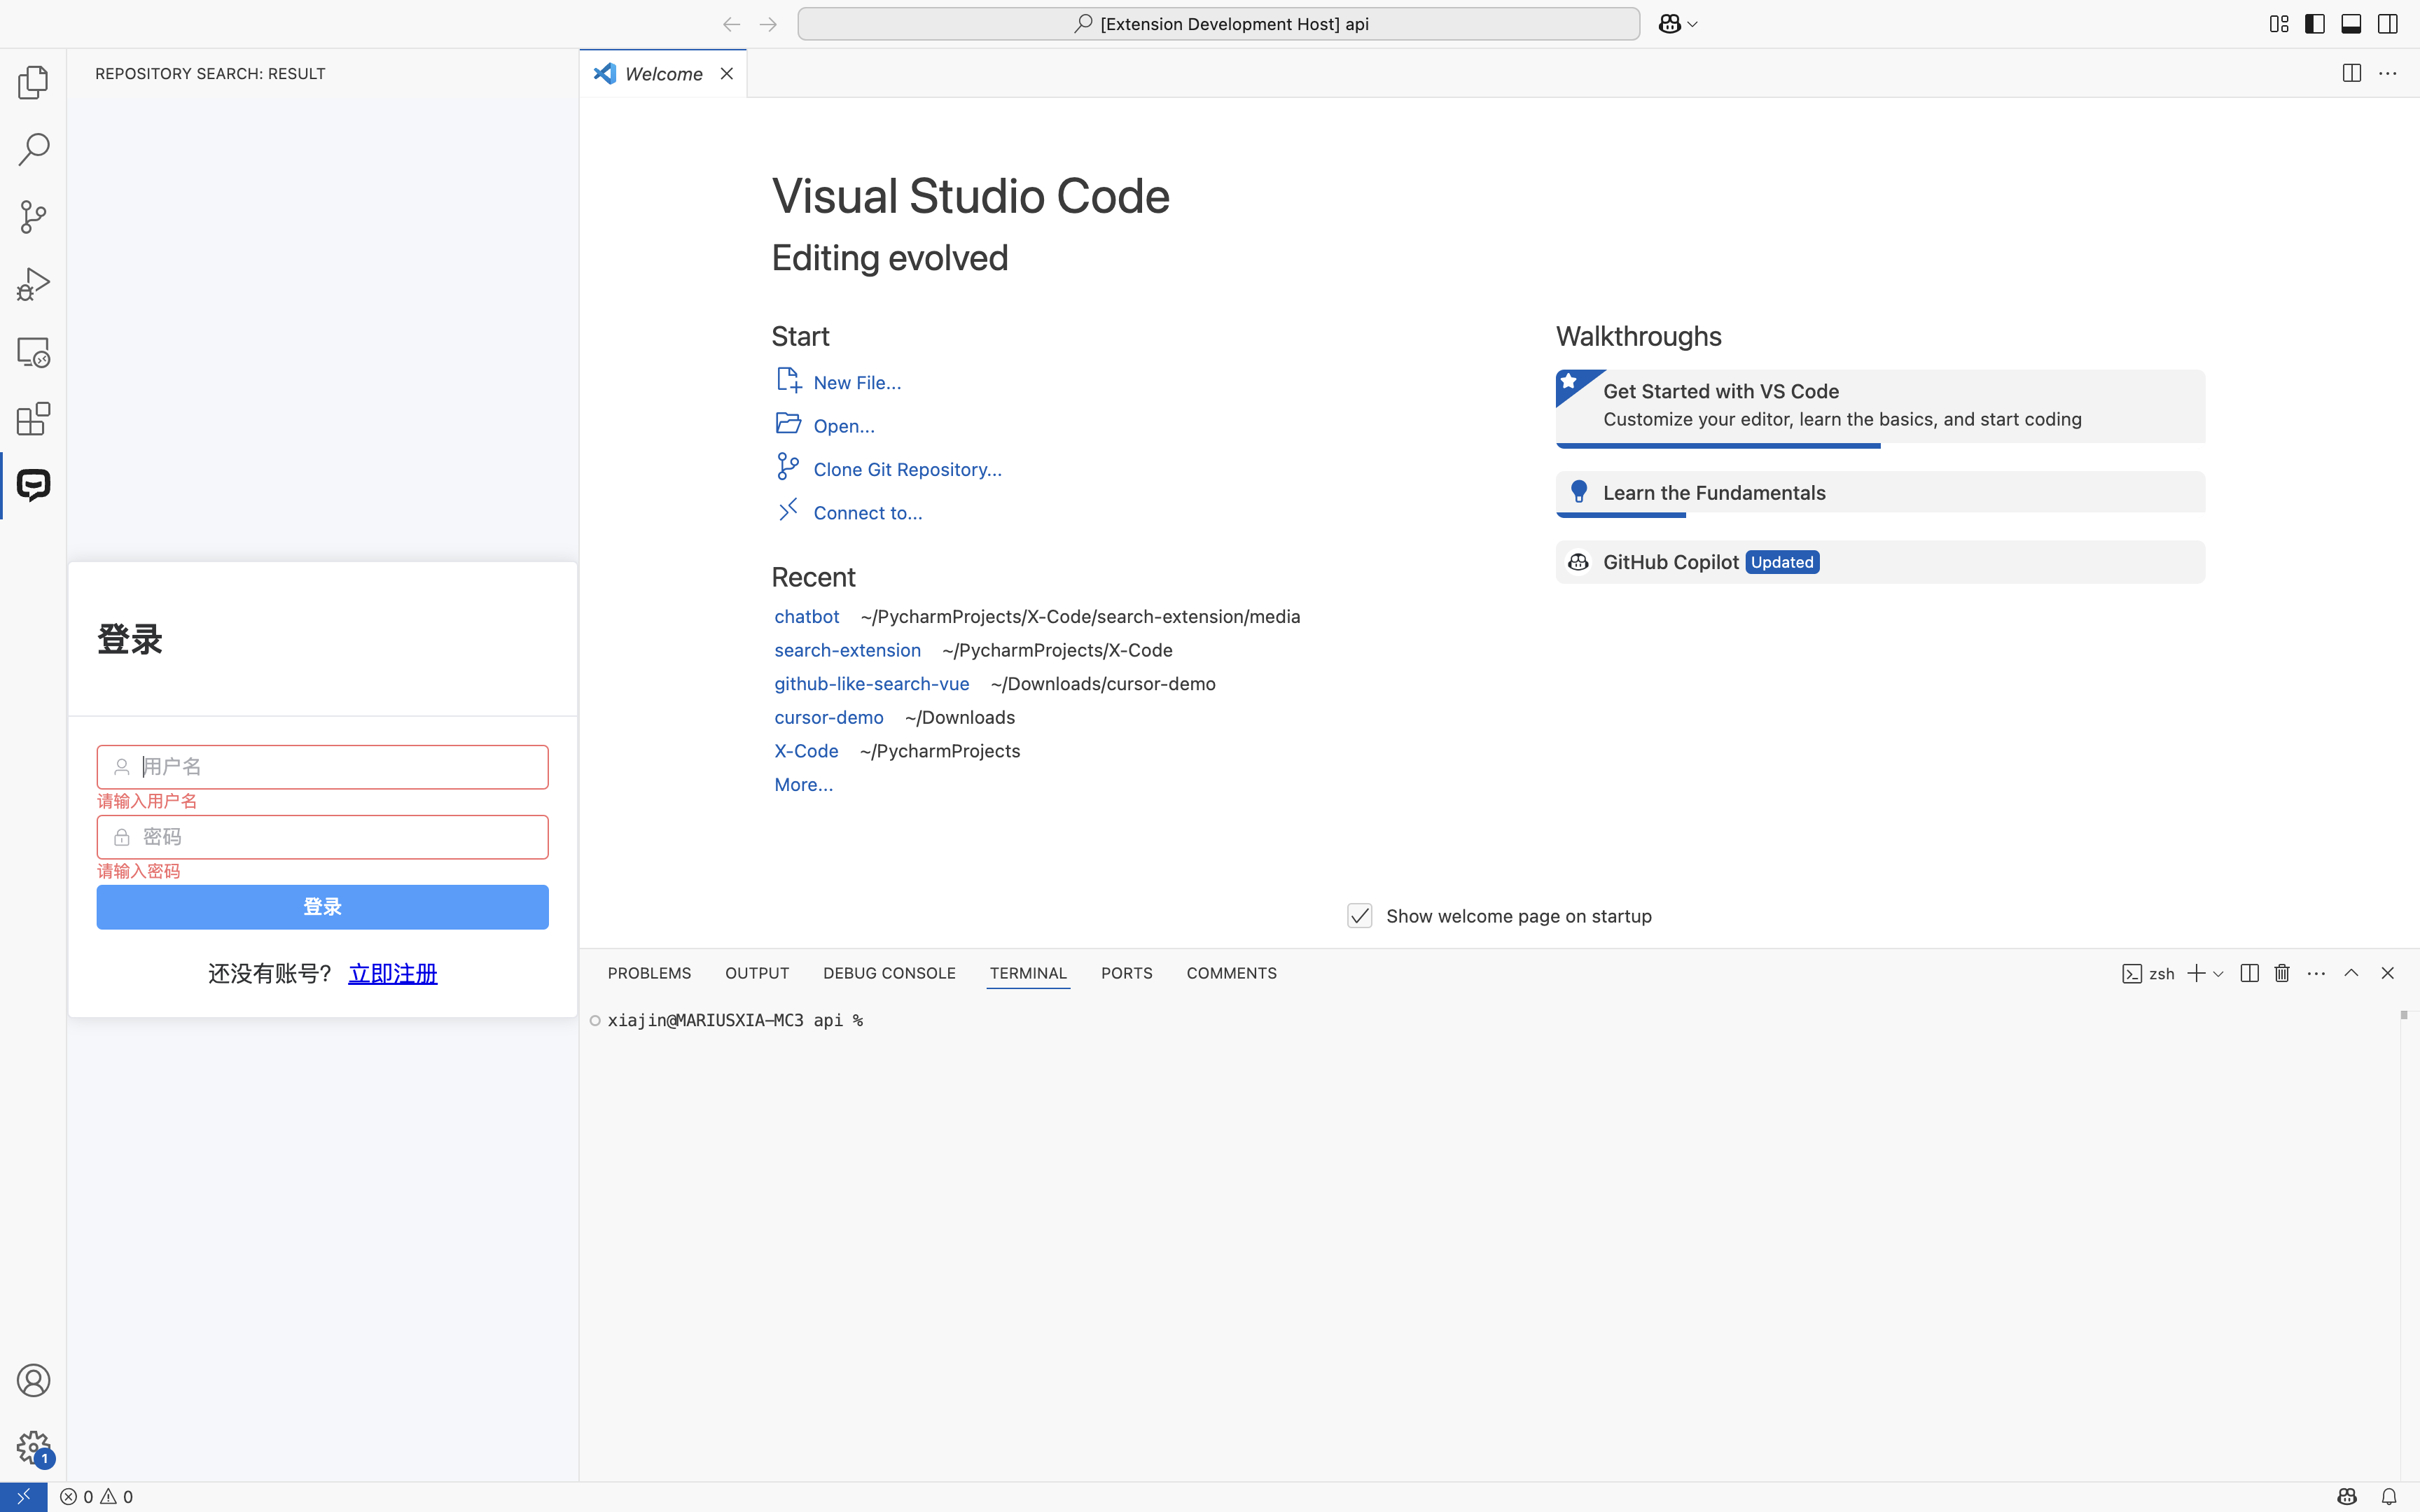
\includegraphics[width=0.95\textwidth]{login_check.png}}
	\caption{登录校验示例}
	\label{logincheck}
\end{figure}
\begin{figure}[H]
	\center{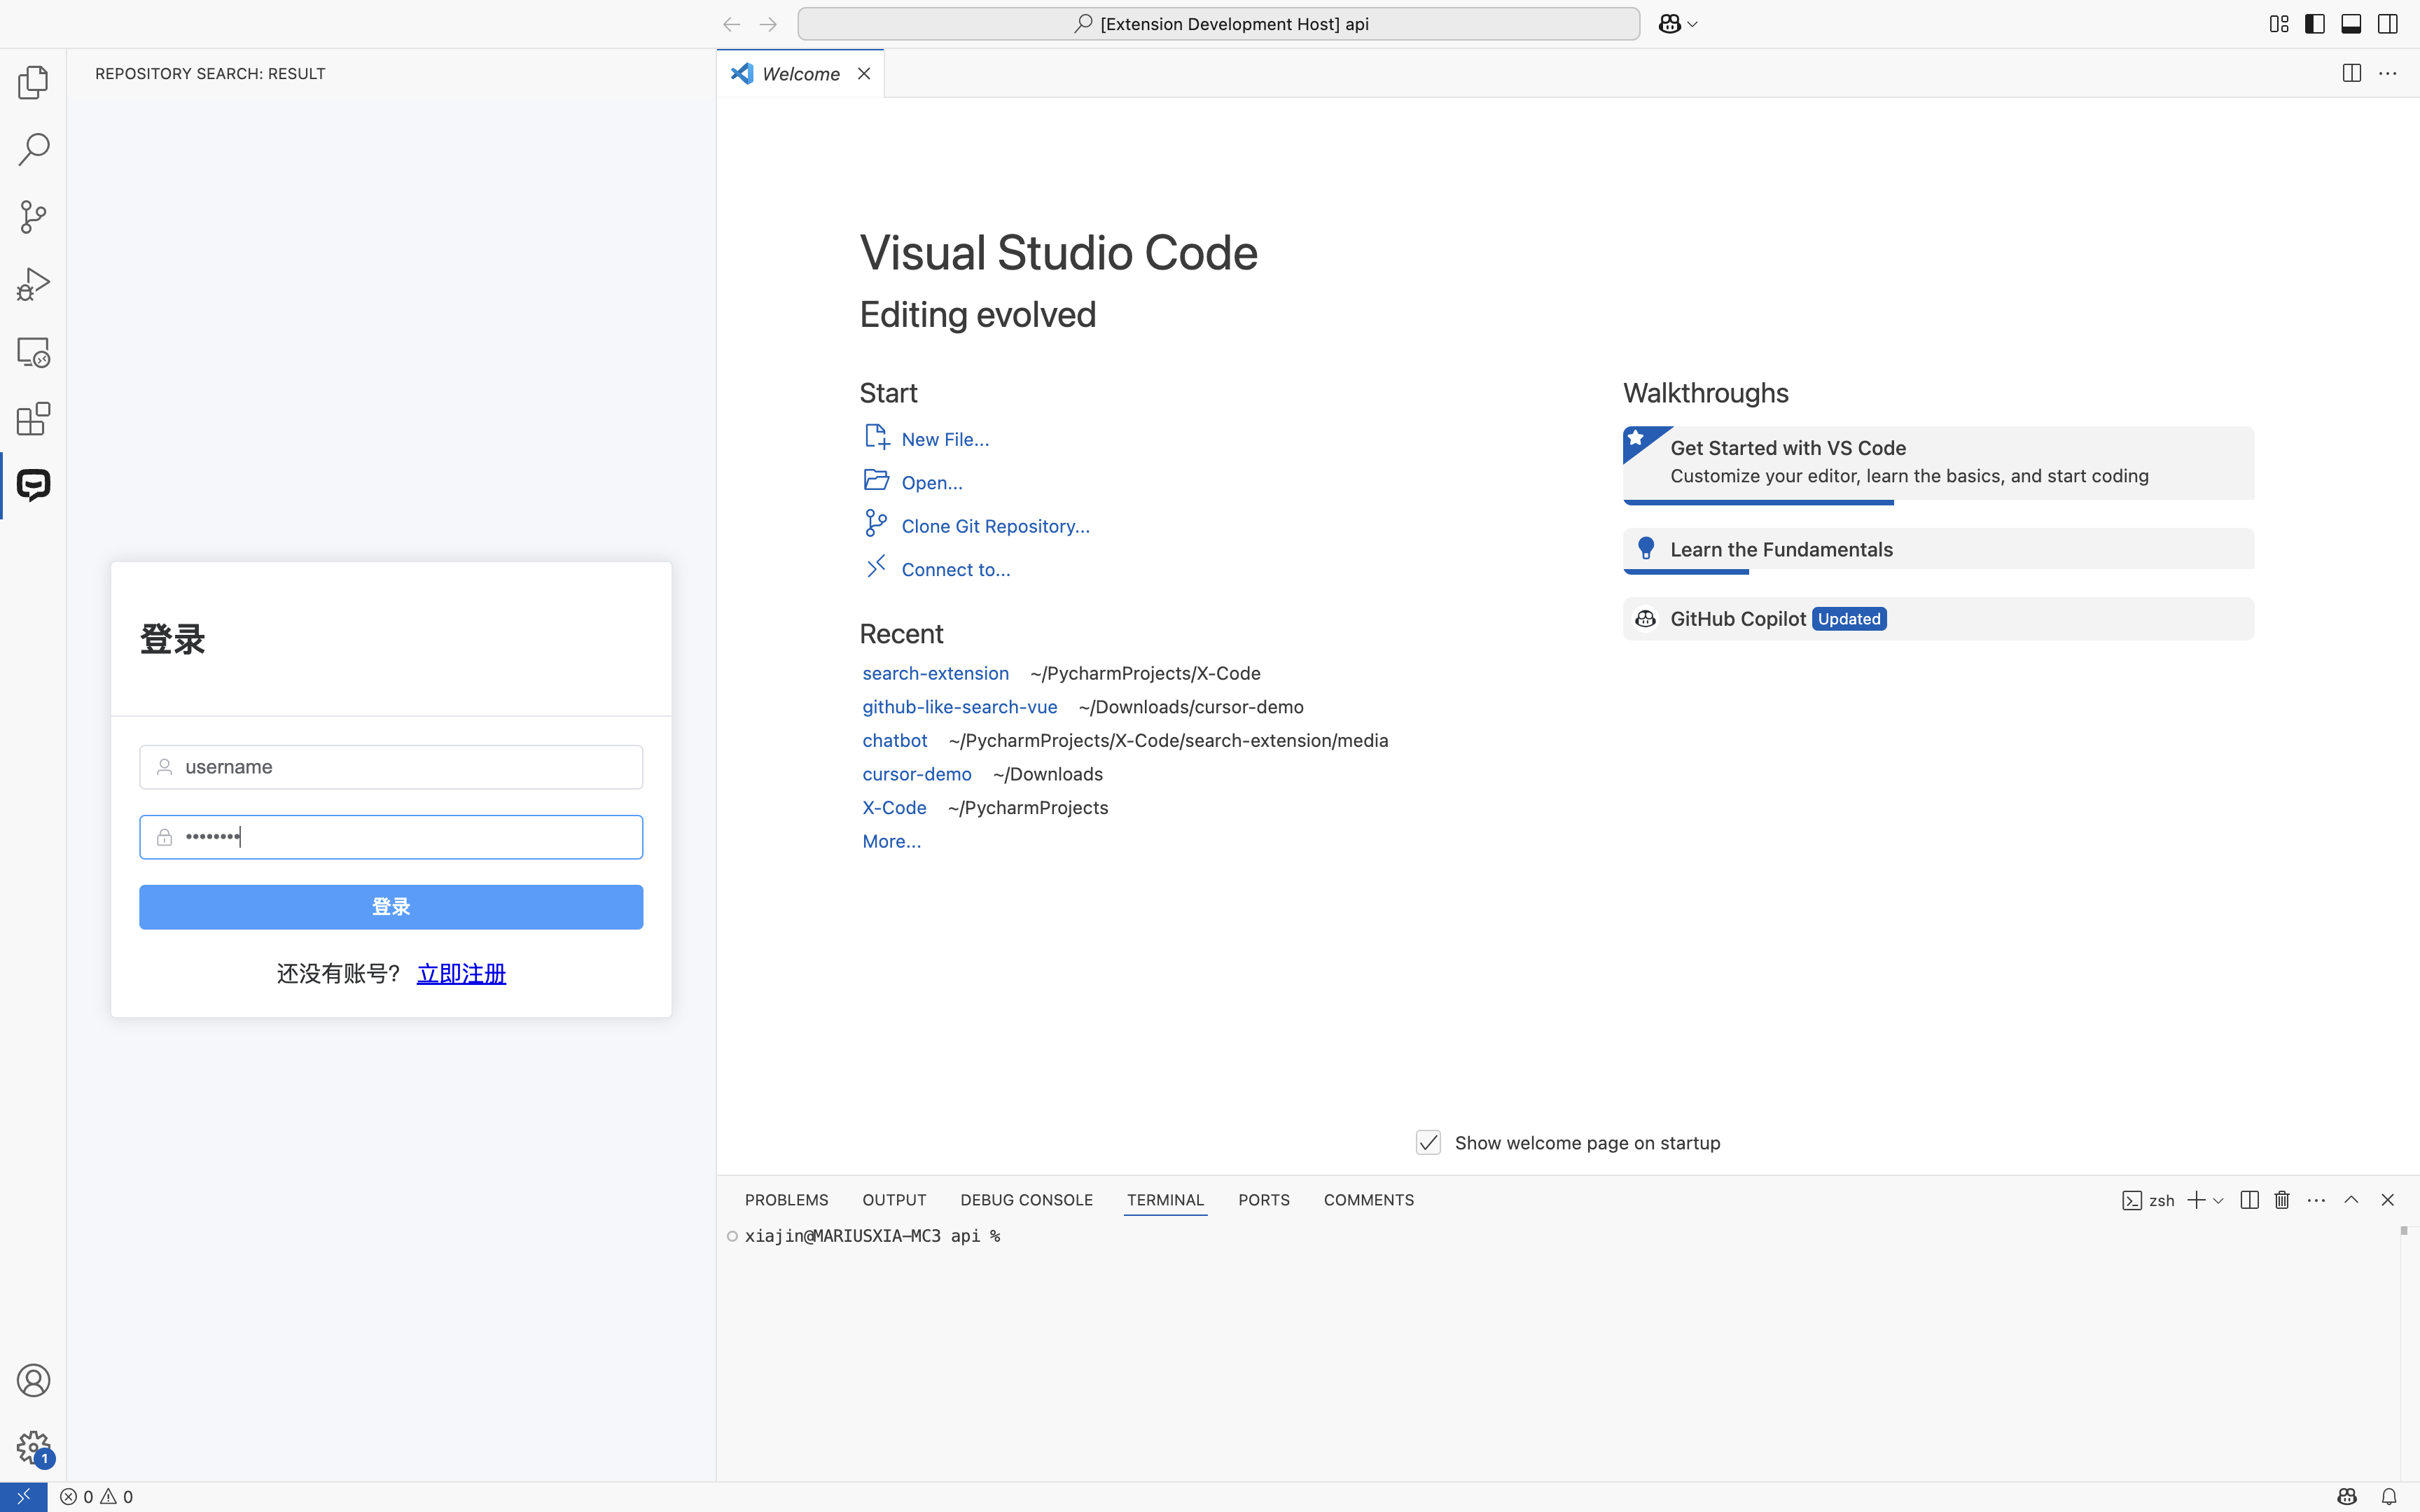
\includegraphics[width=0.95\textwidth]{login.png}}
	\caption{登录示例}
	\label{loginpage}
\end{figure}
注册页面同样拥有完善的输入检测功能,它支持密码一致性校验、邮箱格式验证以及用户名合法性检查,防止无效或者恶意数据被提交。如图\ref{registerpage}和图\ref{registercheckpage}所展示的,系统借助双向数据绑定达成表单状态的实时更新,用户在填写信息时可即刻获得有效性反馈,注册成功之后,系统会自动跳转至登录页面,以此提升用户操作的连贯性。
\begin{figure}[H]
	\center{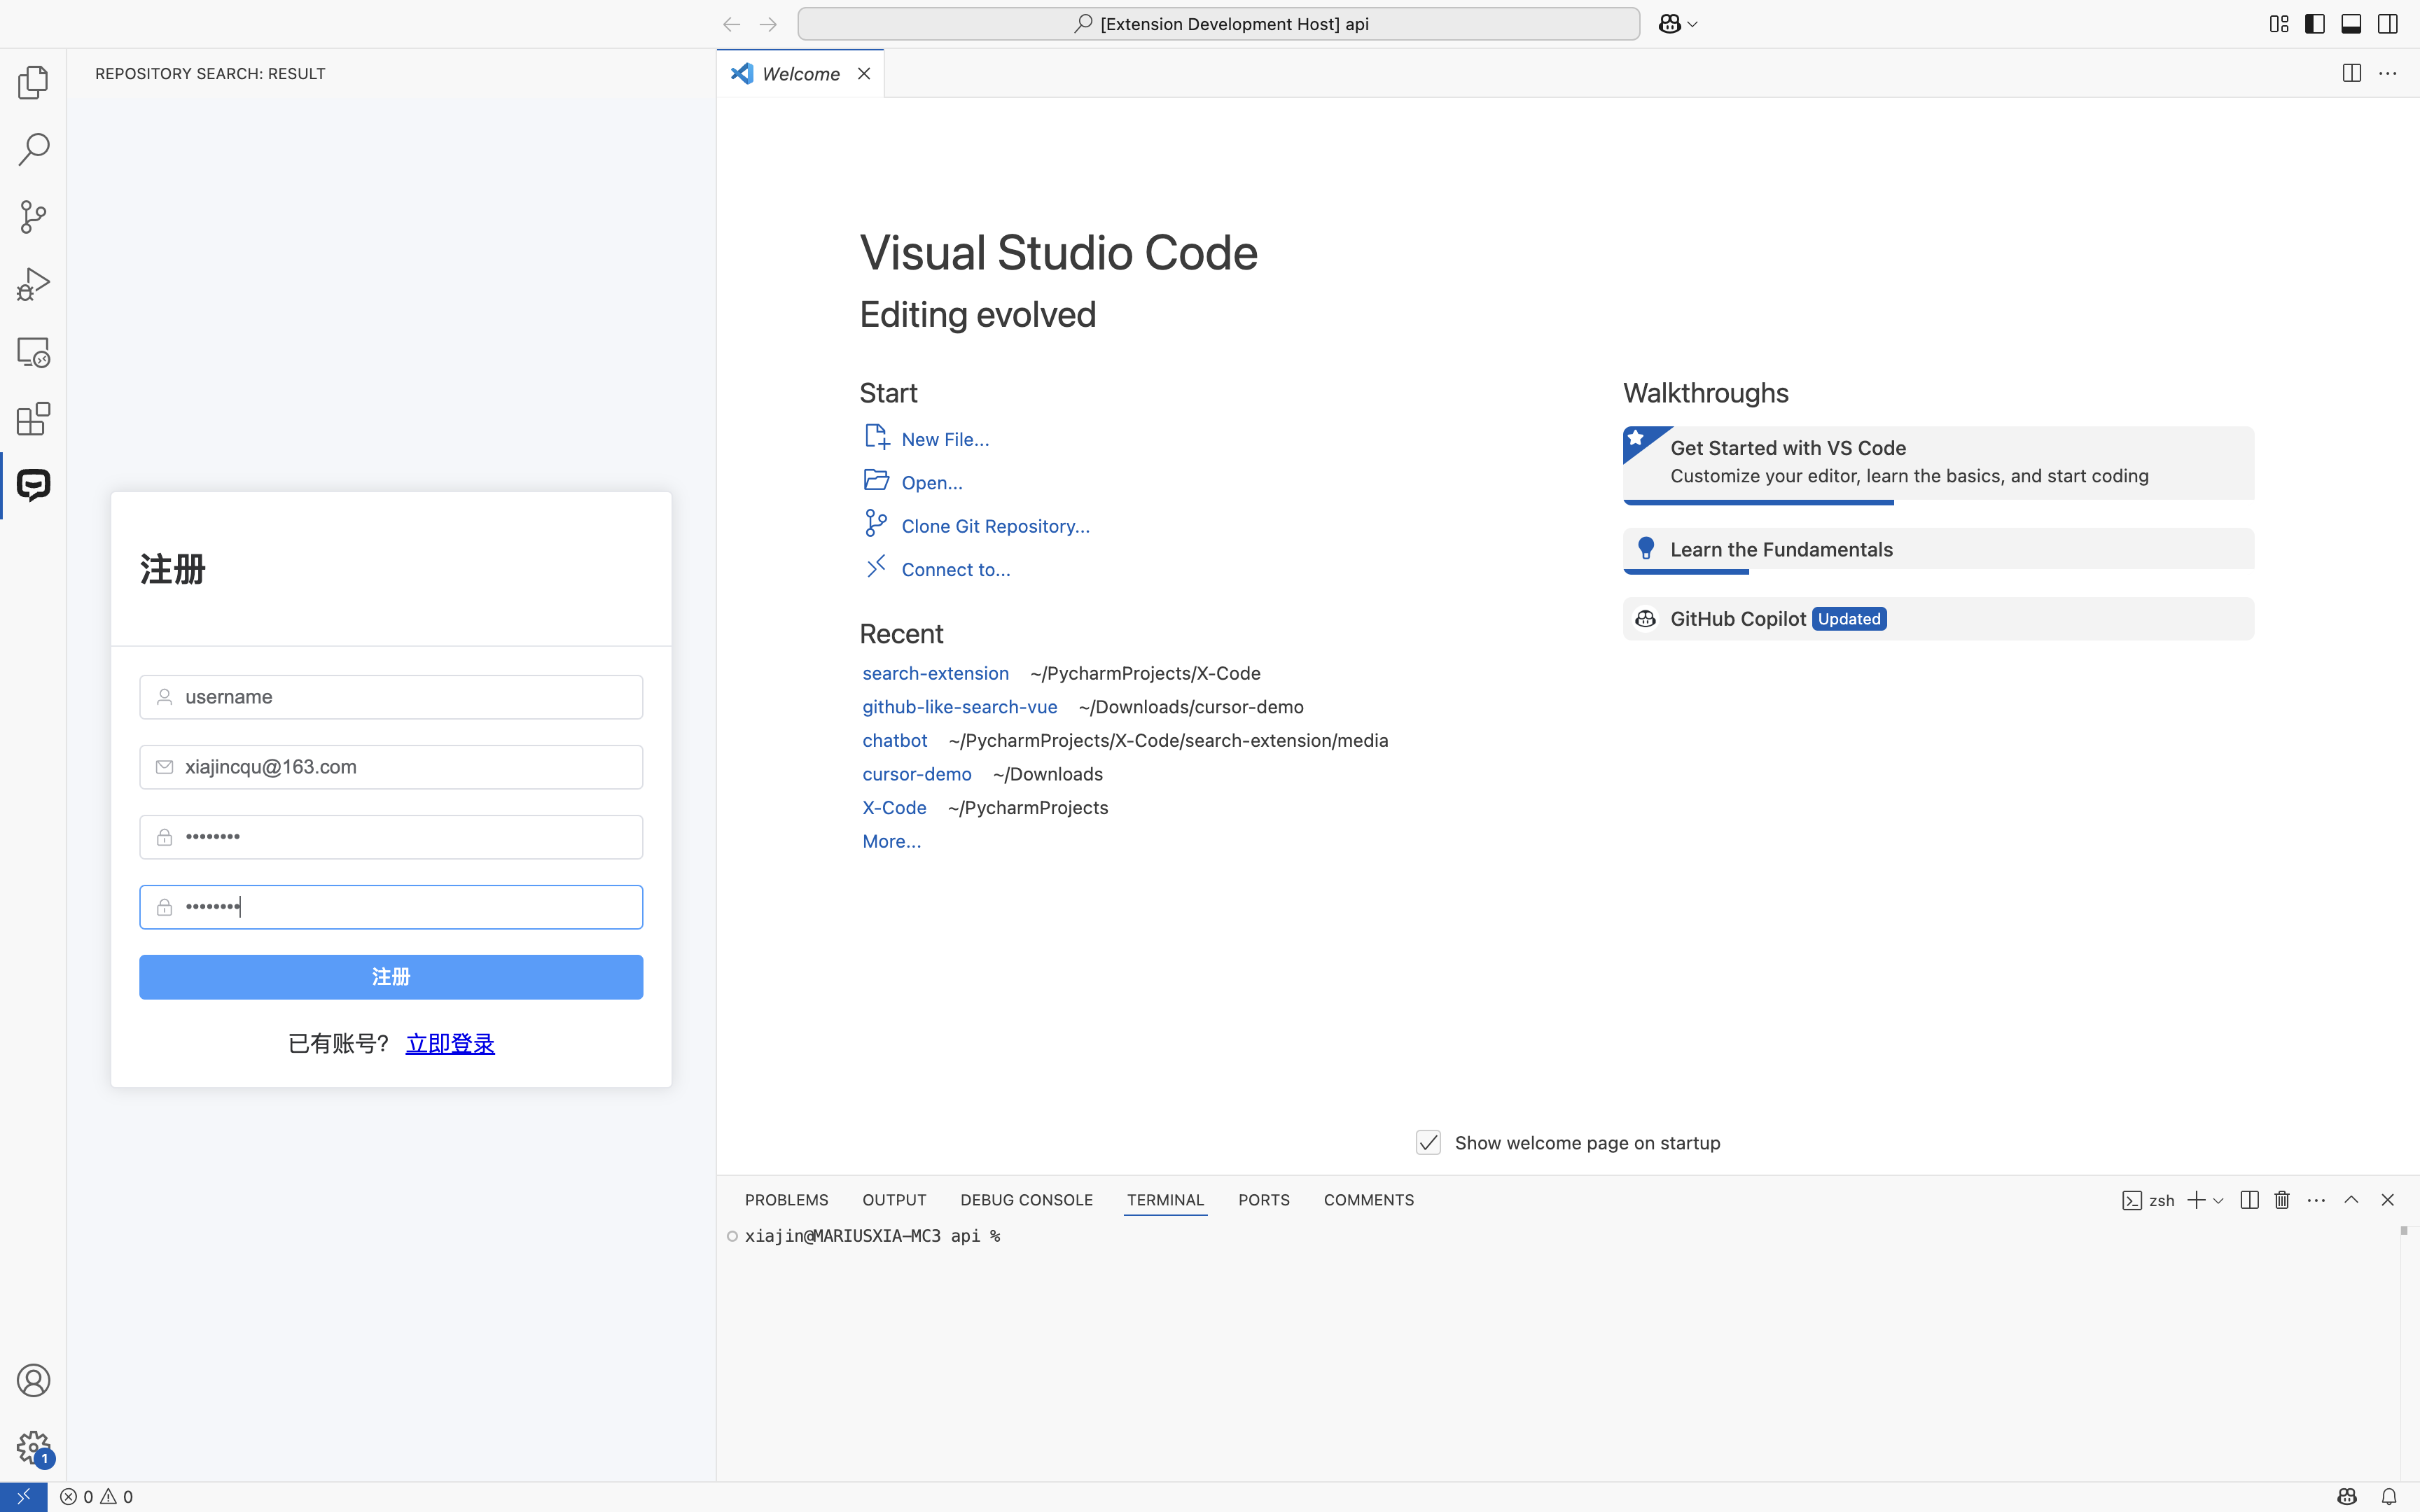
\includegraphics[width=0.95\textwidth]{register.png}}
	\caption{注册示例}
	\label{registerpage}
\end{figure}
\begin{figure}[H]
	\center{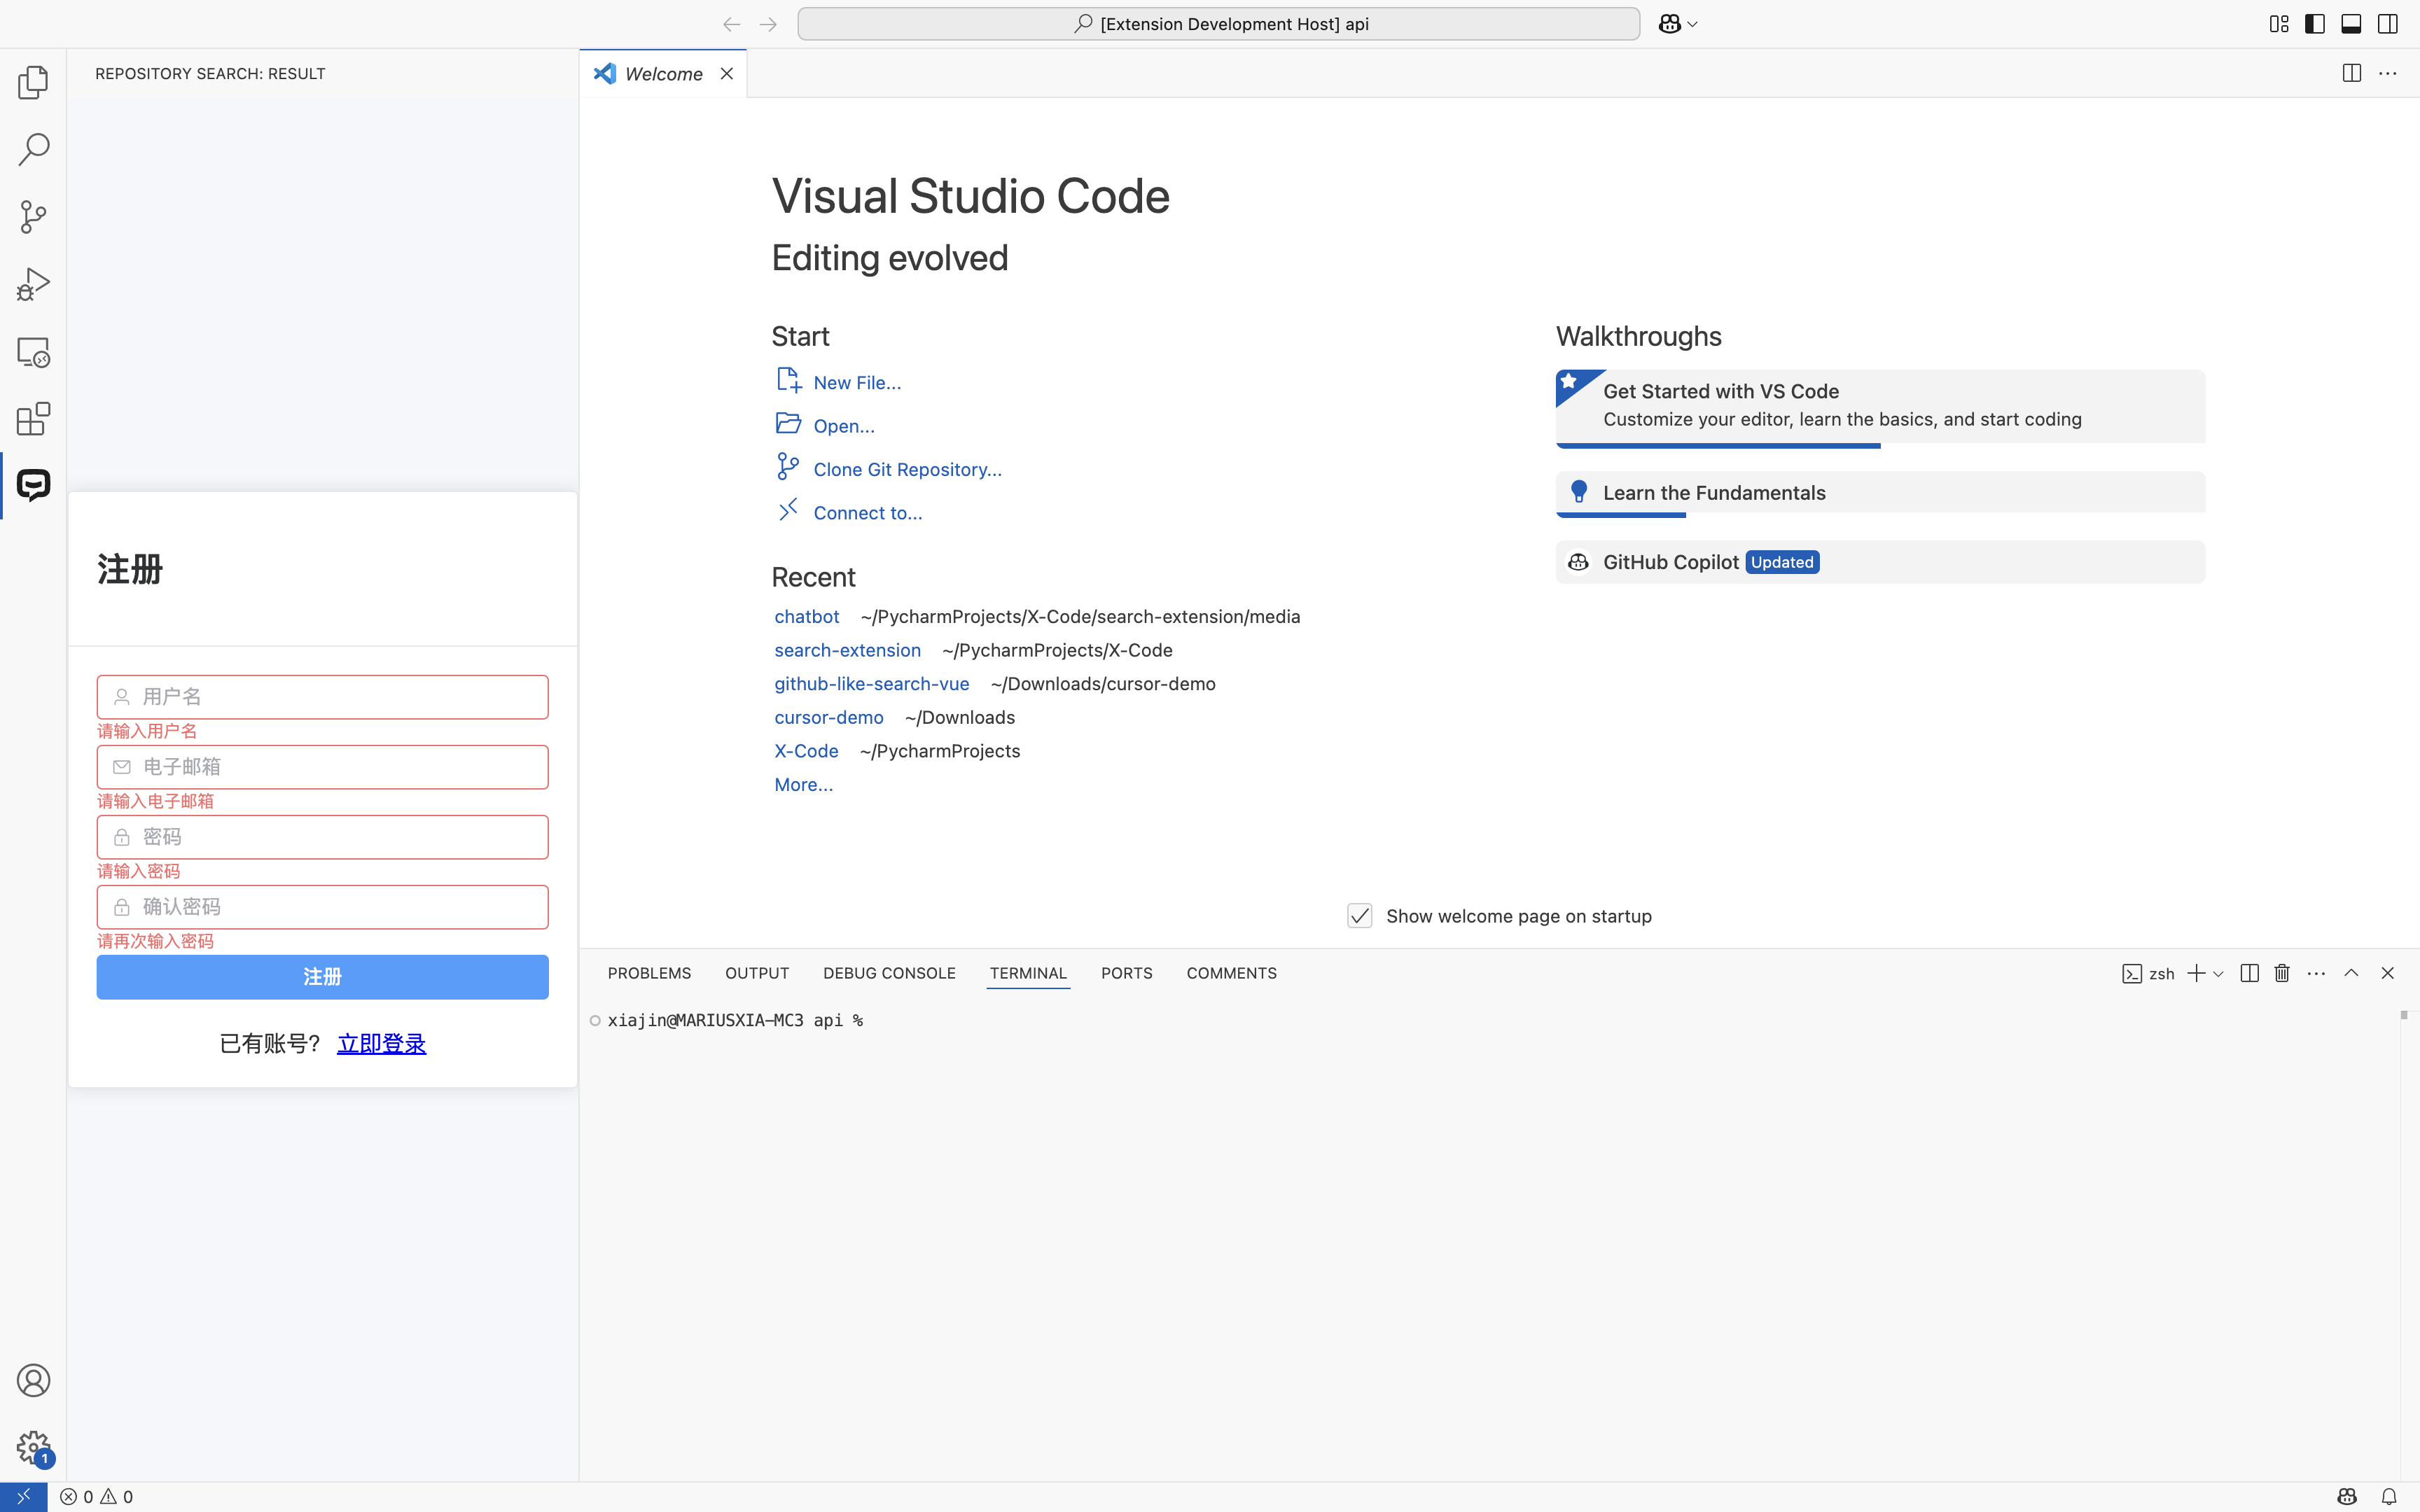
\includegraphics[width=0.95\textwidth]{register_check.png}}
	\caption{注册校验示例}
	\label{registercheckpage}
\end{figure}

系统的搜索页面设计得简洁又直观,用户可在输入框中输入关键词来进行代码检索。和传统搜索引擎不一样,系统在前端对用户输入的查询词开展智能改写和预处理,并且依靠后端专业查询方法获取高质量结果,搜索结果以列表形式呈现,支持项目选中时的高亮动画,以此提升交互体验以及视觉反馈,如图\ref{searchpage}和图\ref{select}所示,用户可借助分页或者滚动加载来查看更多结果,列表项支持快速预览代码片段以及相关元信息,方便用户快速定位目标内容。
\begin{figure}[H]
	\center{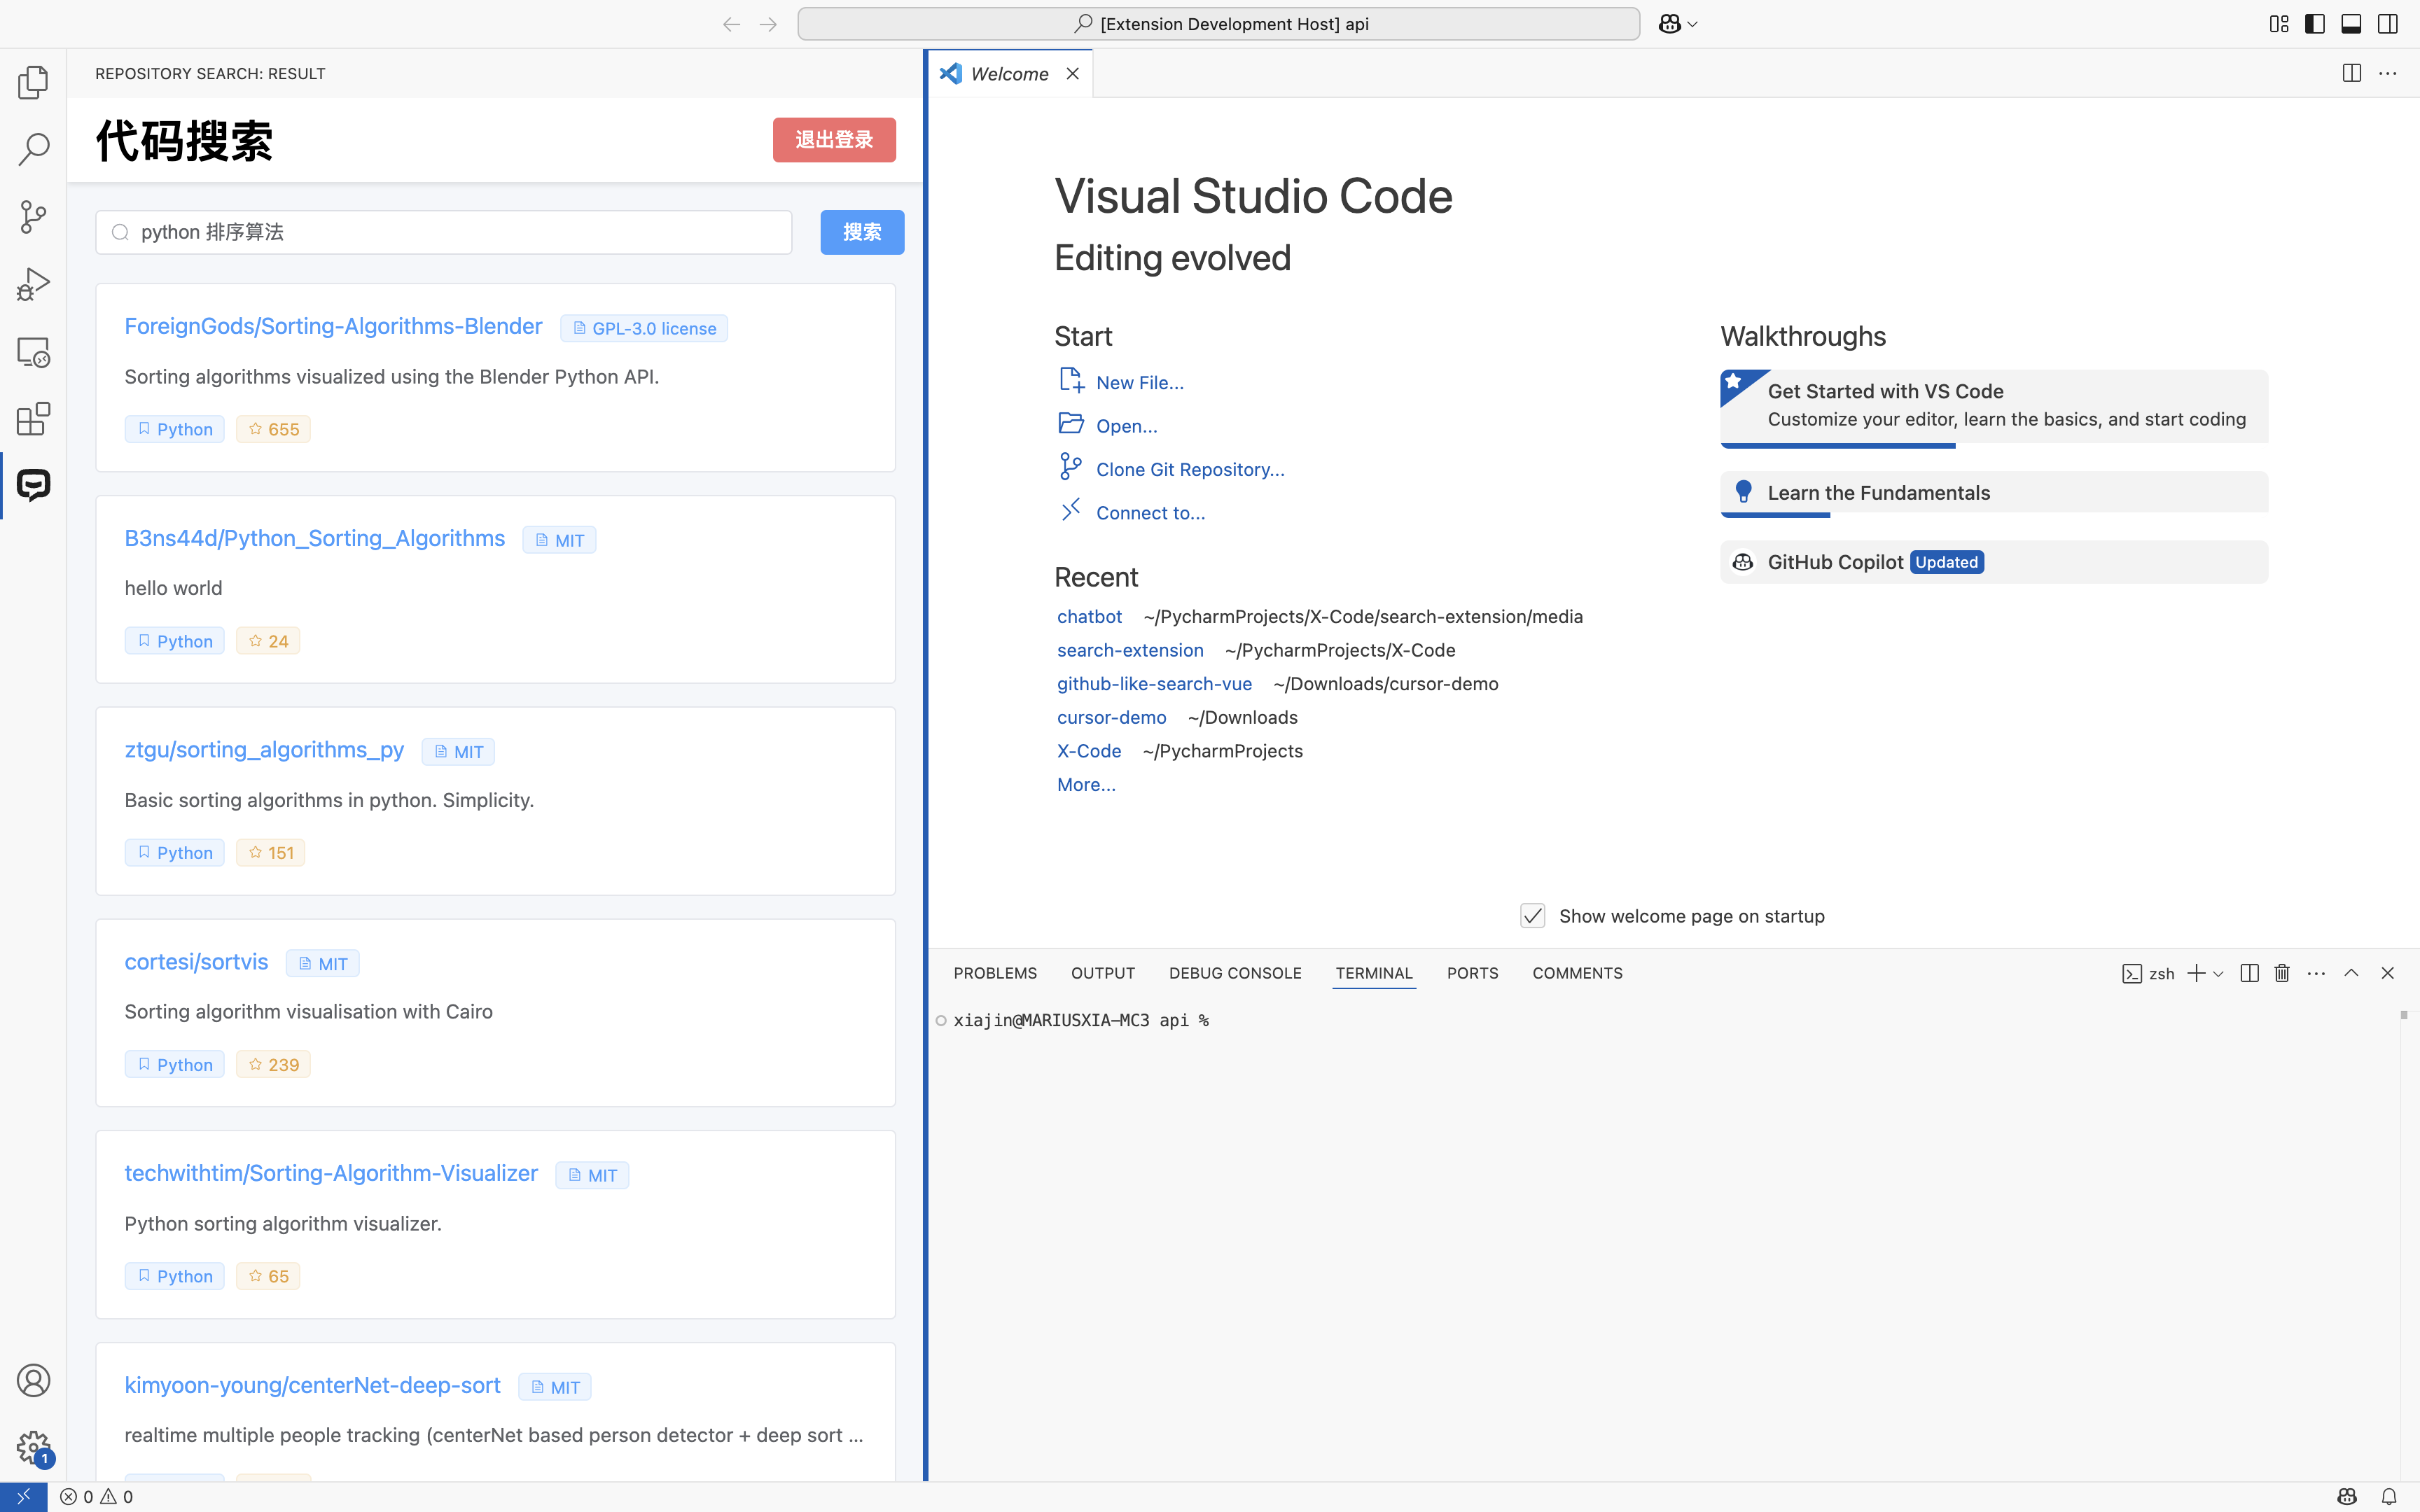
\includegraphics[width=0.95\textwidth]{search_page.png}}
	\caption{搜索页面示例}
	\label{searchpage}
\end{figure}
\begin{figure}[H]
	\center{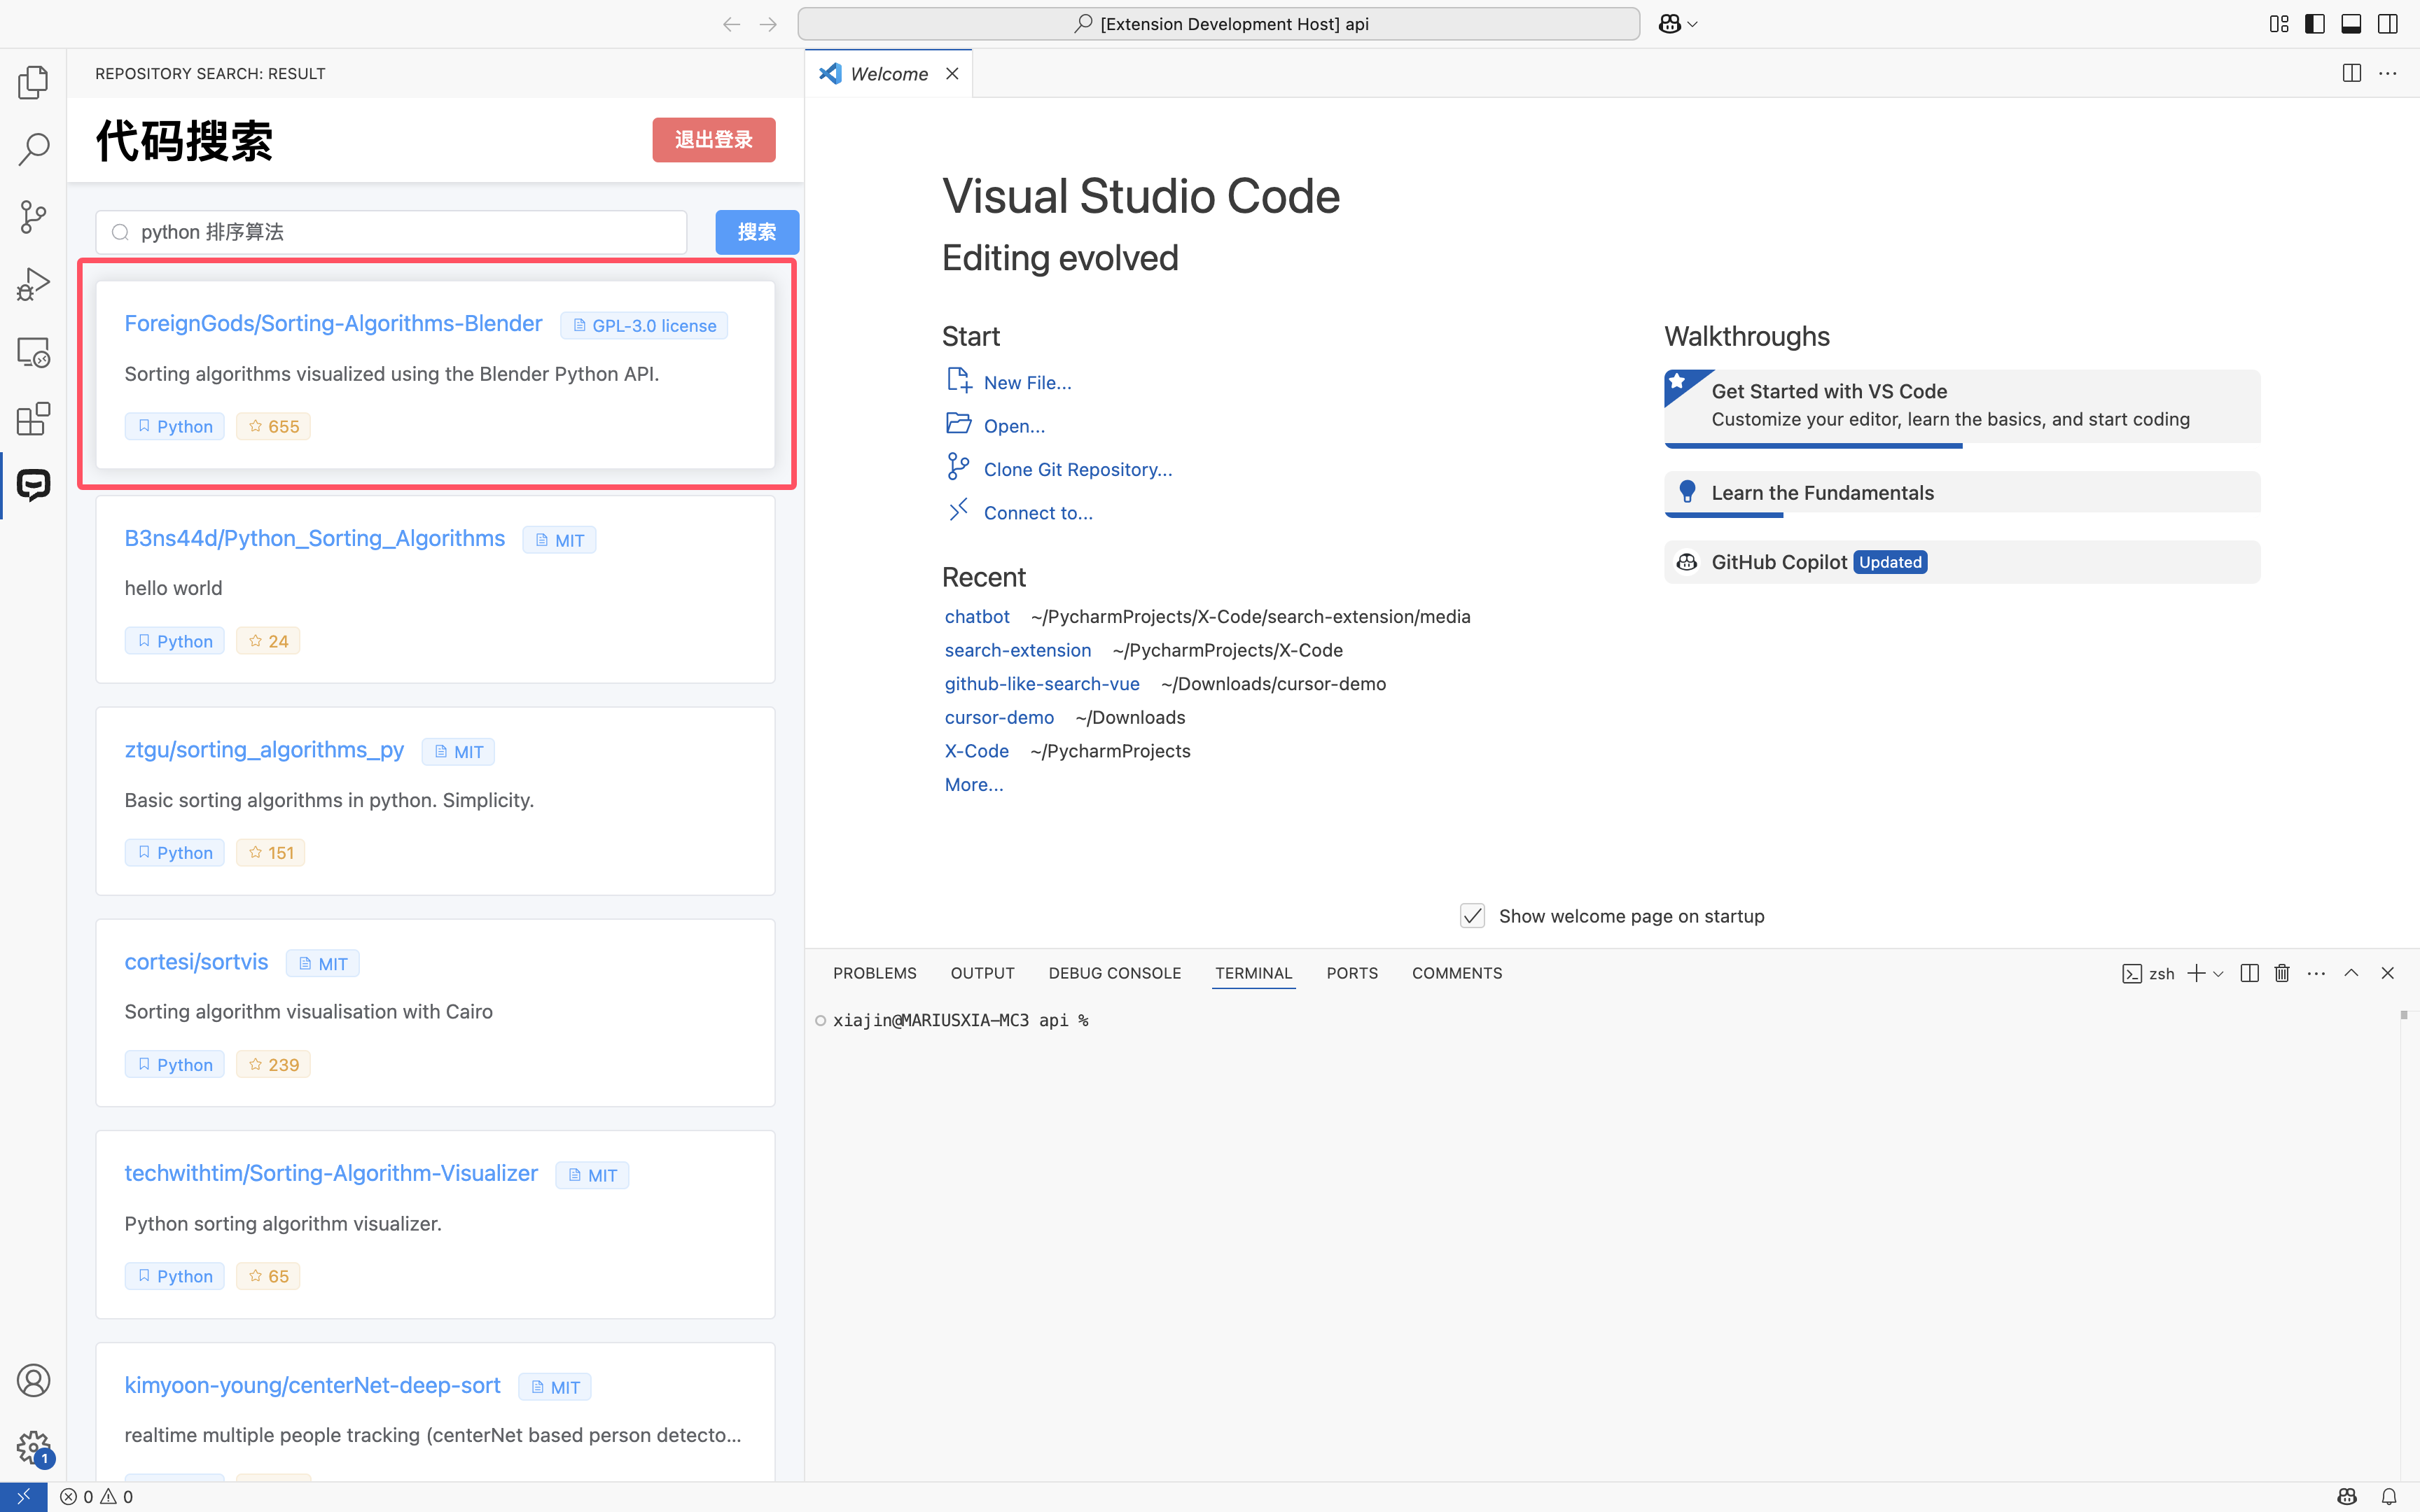
\includegraphics[width=0.95\textwidth]{search_select.png}}
	\caption{选中项目示例}
	\label{select}
\end{figure}
点击某一搜索结果后,用户可进入项目详情页面,该页面详细展示了项目名称、开源协议、项目描述、编程语言、星数、原始链接以及文件列表,支持一键跳转至项目原网页,便于用户浏览和分析,项目详情界面如图\ref{repodetailpage}所示,页面采用模块化布局,信息层次清晰分明,支持文件树结构的动态展开与折叠,以此提升浏览效率。
\begin{figure}[H]
	\center{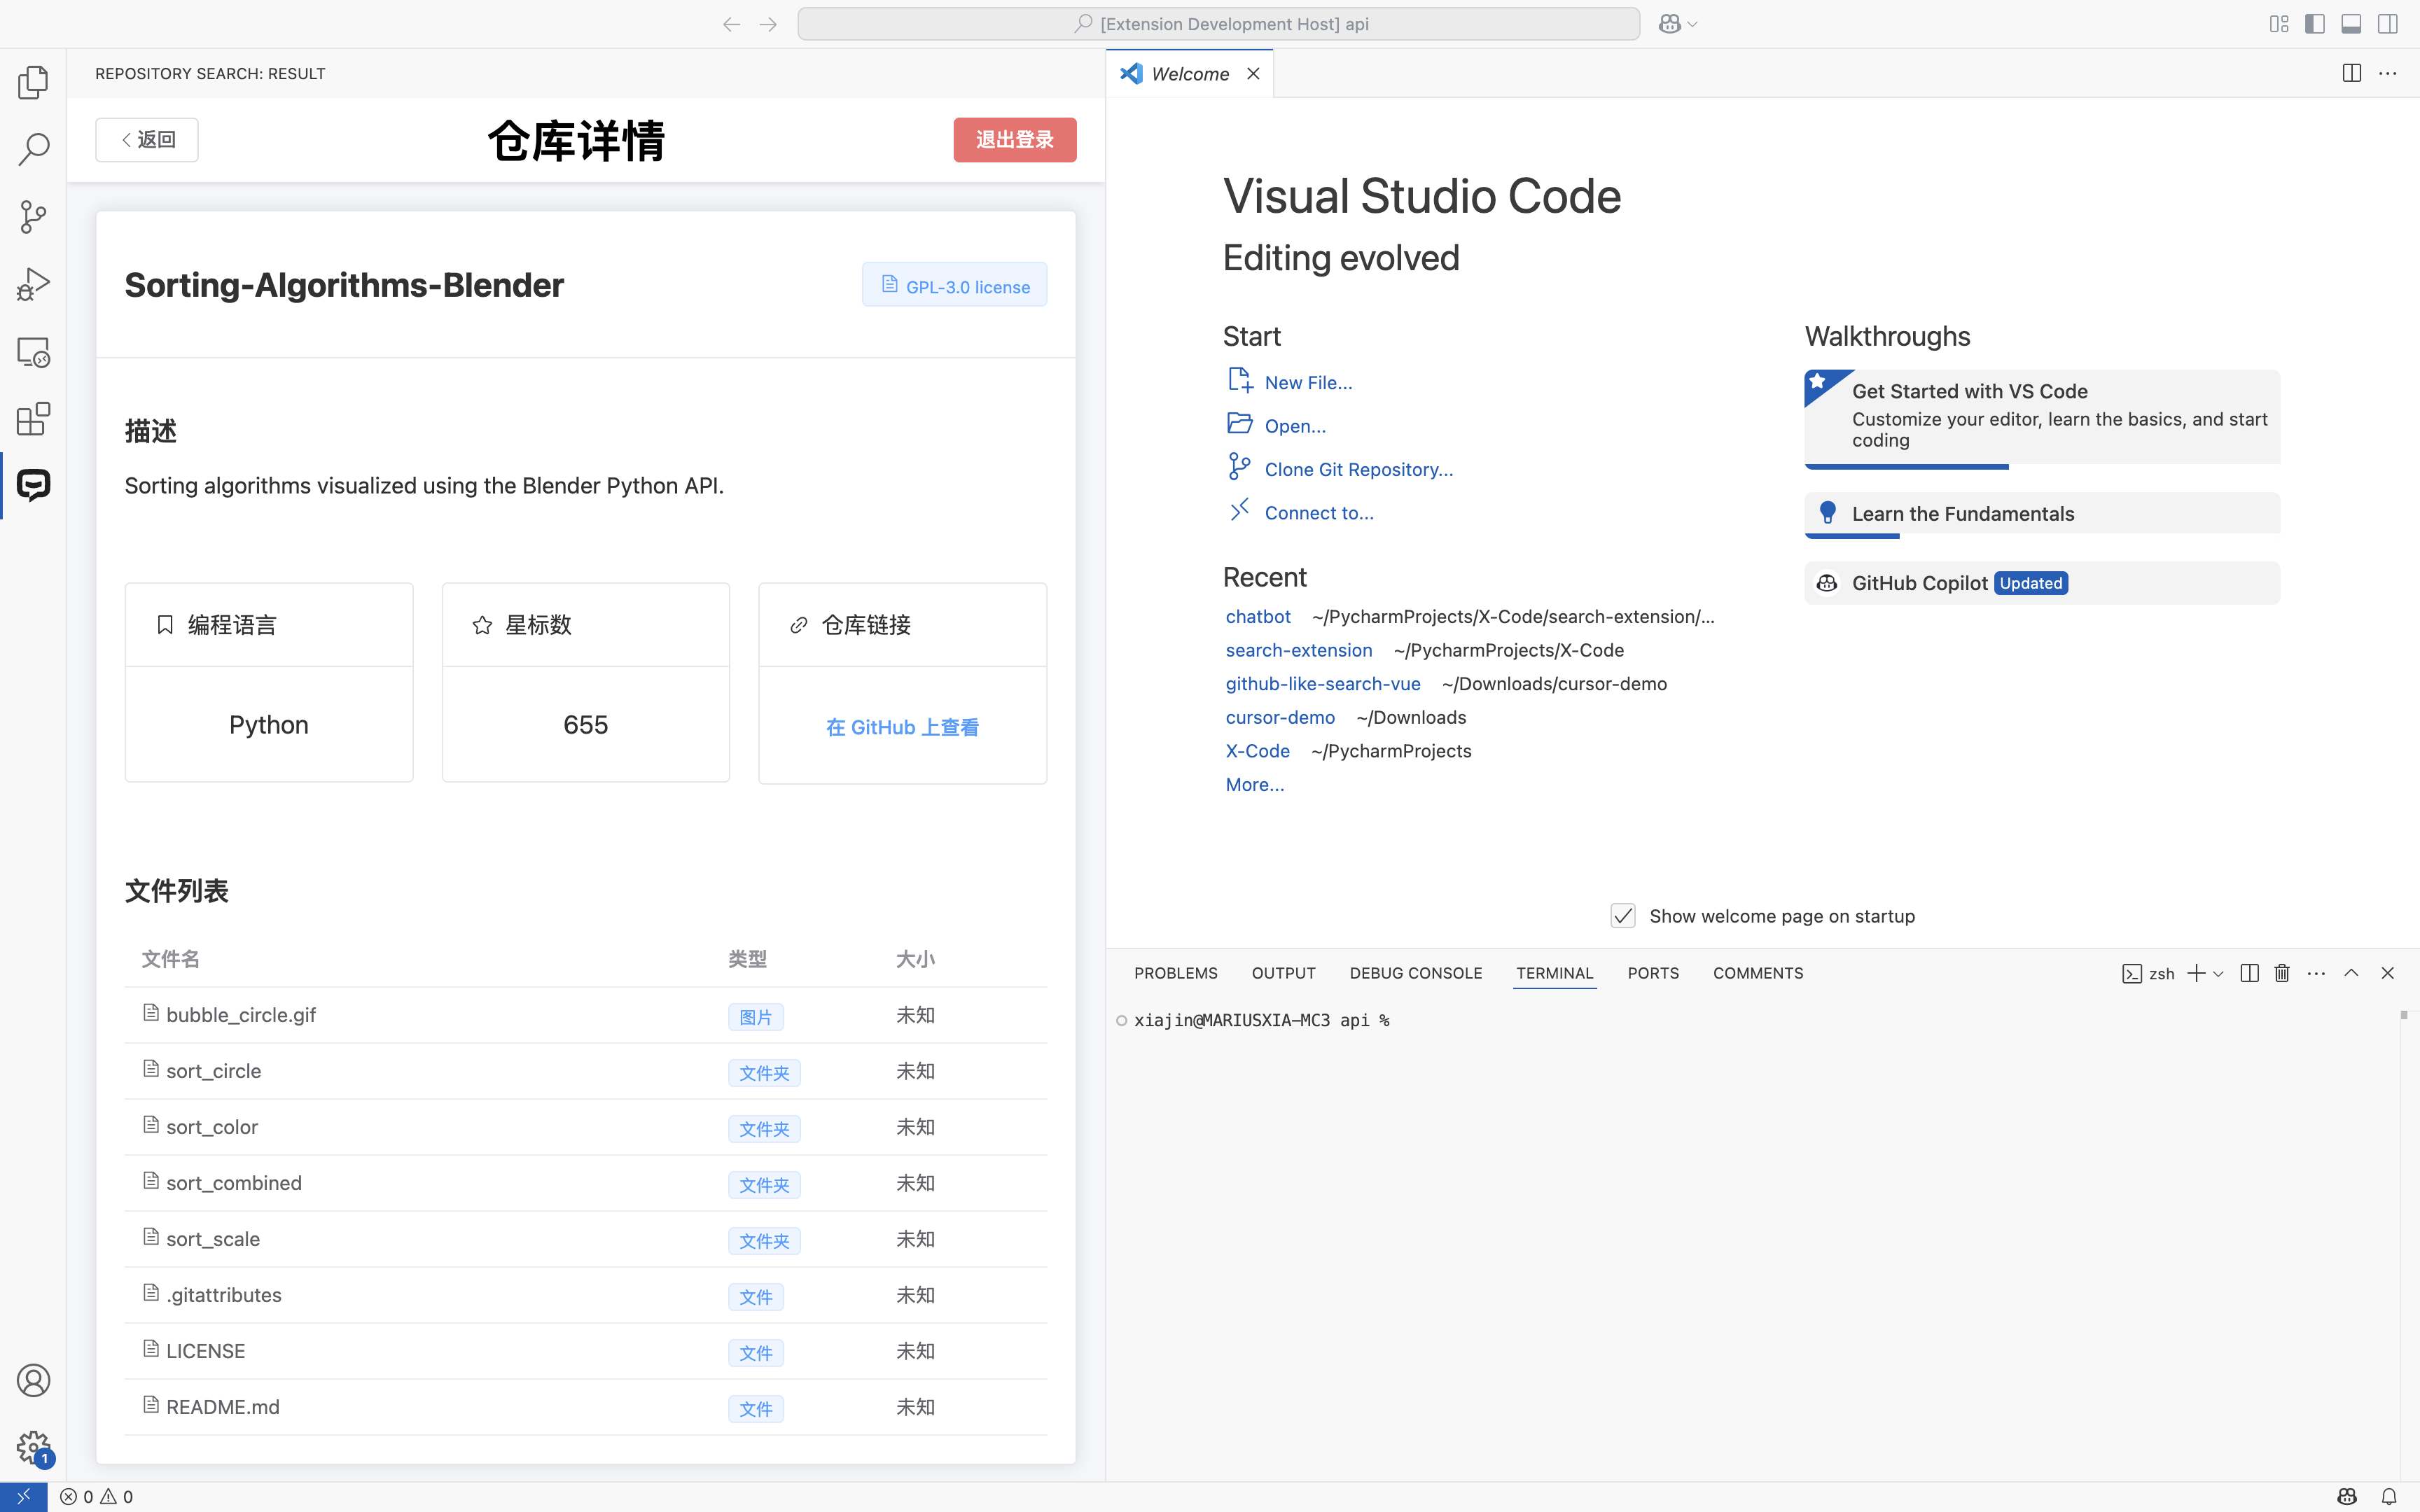
\includegraphics[width=0.95\textwidth]{repo_detail.png}}
	\caption{搜索详情示例}
	\label{repodetailpage}
\end{figure}
前端系统依靠Vuex实现全局状态管理,保证用户登录状态、搜索历史、检索结果等数据在各个页面间同步更新,系统还集成了错误捕获与提示机制,针对网络异常、接口超时等情况给予友好反馈,保障用户操作的连续性以及系统的稳定性,凭借上述多端界面与分层架构的有机结合,系统实现了从用户注册、登录、代码检索到结果展示的完整闭环,有效提升了面向多编程语言的代码检索系统的易用性与用户体验。\par
\subsection{本章小结}
在这一章节当中依据面向多编程语言的代码检索系统所制定的设计方案成功达成了一条囊括代码预处理、后端分布式架构、安全鉴权以及智能检索和前端界面设计的完整技术链路,借助基于AST的多语言代码结构化预处理模块达成了针对不同编程语言源代码的统一解析以及规范化处理,这为后续的语义分析和跨语言检索筑牢了根基。后端选用微服务架构搭建起有高可用性的统一接入网关、鉴权服务以及拥有高性能且可拓展特性的代码查询服务,保证了系统有安全性、稳定性以及高并发处理能力,依赖基于Elasticsearch的高性能分布式查询服务达成了多维度、多语言的精准代码检索,并且结合大语言模型的查询意图理解以及提示词工程提升了检索的质量与结果相关性。在前端层面系统借助Vue框架与VS Code插件的深度融合提供了统一且友善的多端用户体验,支持注册登录的严格校验、智能搜索词预处理、结果高亮展示以及项目详情的模块化浏览,保证了用户操作的流畅性以及系统的易用性,从整体上看这一章节的实现方案充分呈现了系统的模块化设计理念以及技术先进性,为构建高效、智能且安全的多编程语言代码检索平台给予了坚实的技术支撑。\par
\newpage
\fancyhead[LH]{\zihao{-5}{\songti 重庆大学本科学生毕业论文(设计)}}
\fancyhead[RH]{\zihao{-5}{\songti 总结与展望}}

\addcontentsline{toc}{section}{总结与展望}
\renewcommand\refname{总结与展望}
\section*{总结与展望}
本文聚焦面向多编程语言的代码检索系统,提出并实现了一套高效且可扩展、有智能化的技术方案,针对多语言代码的结构化难题,设计了基于AST的统一预处理流程,达成了不同编程语言代码的语法结构对齐以及特征提取,系统采用前后端分离与微服务架构,联合高性能分布式查询引擎Elasticsearch和大语言模型,提升了检索的准确性、扩展性以及系统的高可用性。在安全性方面,系统借助统一网关与鉴权服务,保障了用户数据和服务访问的安全,前端运用Vue框架与VS Code插件,为用户提供了便捷且直观的多端交互体验,凭借提示词工程与上下文提高技术,系统提升了对复杂检索意图的理解和响应能力,整体方案契合了多编程语言环境下的高效代码检索需求,也为后续的智能化代码管理与开发辅助奠定了坚实基础。\par
本项目在研发进程中,一种新的大语言模型协议正在重塑当前基于特定工作流的AI Agent结构,MCP协议,基于大模型的Function Call能力,以一种新方式将外部工具能力接入到大模型Agent中,正在重塑代码检索系统的交互范式与功能边界,未来可将MCP协议深度融入系统架构,凭借动态挂载代码分析工具、调试器、版本管理等外部组件,使检索系统有“智能执行”能力——用户发起检索请求时,系统能返回代码片段,还可基于MCP协议调用工具链自动完成代码补全、错误诊断甚至自动化测试。结合MCP协议的多轮对话机制,可构建更具逻辑性的检索引导流程,凭借智能追问挖掘用户潜在需求,将传统的“被动式检索”升级为“交互式代码创作助手”。\par

\newpage
\fancyhead[LH]{\zihao{-5}{\songti 重庆大学本科学生毕业论文(设计)}}
\fancyhead[RH]{\zihao{-5}{\songti 参考文献}}

\addcontentsline{toc}{section}{参考文献}
\renewcommand\refname{参考文献}

\zihao{5}

\begin{thebibliography}{1}
\setlength{\itemsep}{0pt}
\bibitem{ref0} Gu X, Zhang H, Kim S. Deep code search[C]//Proceedings of the 40th international conference on software engineering. 2018: 933-944.

\bibitem{ref1} Lv F, Zhang H, Lou J, et al. Codehow: Effective code search based on api understanding and extended boolean model (e)[C]//2015 30th IEEE/ACM International Conference on Automated Software Engineering (ASE). IEEE, 2015: 260-270.

\bibitem{ref2} Iyer S, Konstas I, Cheung A, et al. Summarizing source code using a neural attention model[C]//54th Annual Meeting of the Association for Computational Linguistics 2016. Association for Computational Linguistics, 2016: 2073-2083.

\bibitem{ref6} Husain H, Wu H H, Gazit T, et al. Codesearchnet challenge: Evaluating the state of semantic code search[J]. arXiv preprint arXiv:1909.09436, 2019.

\bibitem{ref7} Zhu M, Jain A, Suresh K, et al. Xlcost: A benchmark dataset for cross-lingual code intelligence[J]. arXiv preprint arXiv:2206.08474, 2022.

\bibitem{ref8} Mou L, Jin Z. Tree-based convolutional neural networks: principles and applications[M]. Singapore: Springer, 2018.

\bibitem{ref8.5} Guo D, Ren S, Lu S, et al. Graphcodebert: Pre-training code representations with data flow[J]. arXiv preprint arXiv:2009.08366, 2020.

\bibitem{ref9} Feng Z, Guo D, Tang D, et al. Codebert: A pre-trained model for programming and natural languages[J]. arXiv preprint arXiv:2002.08155, 2020.

\bibitem{ref10} Ahmad W U, Chakraborty S, Ray B, et al. Unified pre-training for program understanding and generation[J]. arXiv preprint arXiv:2103.06333, 2021.

\bibitem{ref11} Guo D, Lu S, Duan N, et al. Unixcoder: Unified cross-modal pre-training for code representation[J]. arXiv preprint arXiv:2203.03850, 2022.

\bibitem{ref12} Shahi D. Apache Solr: an introduction[M]//Apache Solr: A practical approach to enterprise search. Berkeley, CA: Apress, 2015: 1-9.

\bibitem{ref13} Elasticsearch B V. Elasticsearch[J]. software], version, 2018, 6(1).

\bibitem{ref13.5} Chang F, Dean J, Ghemawat S, et al. Bigtable: A distributed storage system for structured data[J]. ACM Transactions on Computer Systems (TOCS), 2008, 26(2): 1-26.

\bibitem{ref13.9} Masse M. REST API design rulebook: designing consistent RESTful web service interfaces[M]. " O'Reilly Media, Inc.", 2011.

\bibitem{ref13.7} Ghomi E J, Rahmani A M, Qader N N. Load-balancing algorithms in cloud computing: A survey[J]. Journal of Network and Computer Applications, 2017, 88: 50-71.

\bibitem{ref14} Vaswani A, Shazeer N, Parmar N, et al. Attention is all you need[J]. Advances in neural information processing systems, 2017, 30.

\bibitem{ref14.5} Sherstinsky A. Fundamentals of recurrent neural network (RNN) and long short-term memory (LSTM) network[J]. Physica D: Nonlinear Phenomena, 2020, 404: 132306.

\bibitem{ref14.7} Vaswani A, Shazeer N, Parmar N, et al. Attention is all you need[J]. Advances in neural information processing systems, 2017, 30.


\bibitem{ref15} Jacobs R A, Jordan M I, Nowlan S J, et al. Adaptive mixtures of local experts[J]. Neural computation, 1991, 3(1): 79-87.

\bibitem{ref16}  Schulhoff S, Ilie M, Balepur N, et al. The prompt report: A systematic survey of prompting techniques[J]. arXiv preprint arXiv:2406.06608, 2024, 5.

\bibitem{ref17} Kojima T, Gu S S, Reid M, et al. Large language models are zero-shot reasoners[J]. Advances in neural information processing systems, 2022, 35: 22199-22213.

\bibitem{ref18} Reynolds L, McDonell K. Prompt programming for large language models: Beyond the few-shot paradigm[C]//Extended abstracts of the 2021 CHI conference on human factors in computing systems. 2021: 1-7.

\bibitem{ref18.5}  De Lauretis L. From monolithic architecture to microservices architecture[C]//2019 IEEE International Symposium on Software Reliability Engineering Workshops (ISSREW). IEEE, 2019: 93-96.


\bibitem{ref19} Indrasiri K, Kuruppu D. gRPC: up and running: building cloud native applications with Go and Java for Docker and Kubernetes[M]. O'Reilly Media, 2020.

\bibitem{ref20} Docker I. Docker[J]. lınea].[Junio de 2017]. Disponible en: https://www. docker. com/what-docker, 2020.

\bibitem{ref21} Kubernetes T. Kubernetes[J]. Kubernetes. Retrieved May, 2019, 24: 2019.


\end{thebibliography}
%(参考文献格式请参考GB/T 7714-2015《信息与文献 参考文献著录规则》)

\newpage
\fancyhead[LH]{\zihao{-5}{\songti 重庆大学本科学生毕业论文(设计)}}
\fancyhead[RH]{\zihao{-5}{\songti 致谢}}

\addcontentsline{toc}{section}{致谢}
\renewcommand\refname{致谢}

\section*{致\quad 谢}
\zihao{-4}
本科四年学习生活在此画上句号。回顾四年学习生活,首先感谢父母对我学业以及人生规划的无条件支持,没有父母的帮助以及支持,也不会有今天我的成就。在学术上,我想感谢肖富元老师对我的科研启蒙,在肖老师实验室里我第一次接触到了科研,也真正的在一个科研领域潜心“钻研”了大半年的时间。无论最后结果如何,都要感谢肖老师对我的科研启蒙指导。刘超、刘老师在我毕业论文上费了相当多心血;同时,在刘老师的实验室中,我第一次接触到了大模型提示词等相关课题,这也是我日后能去到大型互联公司实习的重要跳板,感谢刘老师对我的悉心指导。在我的本科生活中,舒湛老师给予了我生活中莫大的帮助,对我的职业道路起到了关键的影响,在这里也要感谢舒老师对我的谆谆教诲。同时我还要感谢我在腾讯实习期间马博群(mopma),曾喜龙(jasperzeng),李润瑶(ryanli),曲赛(saiqu)对我在职业技能上的引导作用,是我职业道路上最重要的指路石。最后,感谢所有在我本科期间帮助过或是指引过我的朋友们,是他们陪我走过了人生中这精彩的4年。
\newpage
\thispagestyle{empty}

\addcontentsline{toc}{section}{原创性声明和使用授权书}

\includepdf{anc.pdf} 


\end{document} 